\documentclass[twoside]{book}

% Packages required by doxygen
\usepackage{fixltx2e}
\usepackage{calc}
\usepackage{doxygen}
\usepackage[export]{adjustbox} % also loads graphicx
\usepackage{graphicx}
\usepackage[utf8]{inputenc}
\usepackage{makeidx}
\usepackage{multicol}
\usepackage{multirow}
\PassOptionsToPackage{warn}{textcomp}
\usepackage{textcomp}
\usepackage[nointegrals]{wasysym}
\usepackage[table]{xcolor}

% Font selection
\usepackage[T1]{fontenc}
\usepackage[scaled=.90]{helvet}
\usepackage{courier}
\usepackage{amssymb}
\usepackage{sectsty}
\renewcommand{\familydefault}{\sfdefault}
\allsectionsfont{%
  \fontseries{bc}\selectfont%
  \color{darkgray}%
}
\renewcommand{\DoxyLabelFont}{%
  \fontseries{bc}\selectfont%
  \color{darkgray}%
}
\newcommand{\+}{\discretionary{\mbox{\scriptsize$\hookleftarrow$}}{}{}}

% Page & text layout
\usepackage{geometry}
\geometry{%
  a4paper,%
  top=2.5cm,%
  bottom=2.5cm,%
  left=2.5cm,%
  right=2.5cm%
}
\tolerance=750
\hfuzz=15pt
\hbadness=750
\setlength{\emergencystretch}{15pt}
\setlength{\parindent}{0cm}
\setlength{\parskip}{0.2cm}
\makeatletter
\renewcommand{\paragraph}{%
  \@startsection{paragraph}{4}{0ex}{-1.0ex}{1.0ex}{%
    \normalfont\normalsize\bfseries\SS@parafont%
  }%
}
\renewcommand{\subparagraph}{%
  \@startsection{subparagraph}{5}{0ex}{-1.0ex}{1.0ex}{%
    \normalfont\normalsize\bfseries\SS@subparafont%
  }%
}
\makeatother

% Headers & footers
\usepackage{fancyhdr}
\pagestyle{fancyplain}
\fancyhead[LE]{\fancyplain{}{\bfseries\thepage}}
\fancyhead[CE]{\fancyplain{}{}}
\fancyhead[RE]{\fancyplain{}{\bfseries\leftmark}}
\fancyhead[LO]{\fancyplain{}{\bfseries\rightmark}}
\fancyhead[CO]{\fancyplain{}{}}
\fancyhead[RO]{\fancyplain{}{\bfseries\thepage}}
\fancyfoot[LE]{\fancyplain{}{}}
\fancyfoot[CE]{\fancyplain{}{}}
\fancyfoot[RE]{\fancyplain{}{\bfseries\scriptsize Generated on Tue Oct 13 2015 13\+:00\+:27 for gro-\/microcontroller by Doxygen }}
\fancyfoot[LO]{\fancyplain{}{\bfseries\scriptsize Generated on Tue Oct 13 2015 13\+:00\+:27 for gro-\/microcontroller by Doxygen }}
\fancyfoot[CO]{\fancyplain{}{}}
\fancyfoot[RO]{\fancyplain{}{}}
\renewcommand{\footrulewidth}{0.4pt}
\renewcommand{\chaptermark}[1]{%
  \markboth{#1}{}%
}
\renewcommand{\sectionmark}[1]{%
  \markright{\thesection\ #1}%
}

% Indices & bibliography
\usepackage{natbib}
\usepackage[titles]{tocloft}
\setcounter{tocdepth}{3}
\setcounter{secnumdepth}{5}
\makeindex

% Hyperlinks (required, but should be loaded last)
\usepackage{ifpdf}
\ifpdf
  \usepackage[pdftex,pagebackref=true]{hyperref}
\else
  \usepackage[ps2pdf,pagebackref=true]{hyperref}
\fi
\hypersetup{%
  colorlinks=true,%
  linkcolor=blue,%
  citecolor=blue,%
  unicode%
}

% Custom commands
\newcommand{\clearemptydoublepage}{%
  \newpage{\pagestyle{empty}\cleardoublepage}%
}


%===== C O N T E N T S =====

\begin{document}

% Titlepage & ToC
\hypersetup{pageanchor=false,
             bookmarks=true,
             bookmarksnumbered=true,
             pdfencoding=unicode
            }
\pagenumbering{roman}
\begin{titlepage}
\vspace*{7cm}
\begin{center}%
{\Large gro-\/microcontroller }\\
\vspace*{1cm}
{\large Generated by Doxygen 1.8.9.1}\\
\vspace*{0.5cm}
{\small Tue Oct 13 2015 13:00:27}\\
\end{center}
\end{titlepage}
\clearemptydoublepage
\tableofcontents
\clearemptydoublepage
\pagenumbering{arabic}
\hypersetup{pageanchor=true}

%--- Begin generated contents ---
\chapter{Groduino}
\label{index}\hypertarget{index}{}\begin{DoxyAuthor}{Author}
Jake Rye
\end{DoxyAuthor}
This is the microcontroller code. It is uploaded to the Arduino Mega. It\textquotesingle{}s purpose is to be the firmware for applicable sensor/actuator modules. It has been written in such a way that each new type of sensor and actuator is its own module. Each sensor/actuator module must contain a class with the following methods\+: void begin(void), String get(void), String set(\+String instruction\+\_\+code, int instruction\+\_\+id, String instruction\+\_\+parameter). The existance of these methods are enforced by using the \hyperlink{class_sensor_actuator_module}{Sensor\+Actuator\+Module} interface. Each sensor/actuator must also be instantiated such that its modularity is prioritized. For example, passing in pins, instruction codes, and instruction ids (all parameters that are subject to change depending on the context the module is used in) would look something like\+: Module\+Name(int pin, String instruction\+\_\+code, int instruction\+\_\+id). Clearly this example is not representative of all modules that will be created so it is up to the programmer to use their best judgement. Another important note is that this code documentation is generated with doxygen so all markdown should follow compliant formats. 
\chapter{Hierarchical Index}
\section{Class Hierarchy}
This inheritance list is sorted roughly, but not completely, alphabetically\+:\begin{DoxyCompactList}
\item \contentsline{section}{Communication}{\pageref{class_communication}}{}
\item \contentsline{section}{Instruction}{\pageref{struct_instruction}}{}
\item \contentsline{section}{Moving\+Average\+Filter}{\pageref{class_moving_average_filter}}{}
\item \contentsline{section}{One\+Wire}{\pageref{class_one_wire}}{}
\item \contentsline{section}{Sensor\+Actuator\+Module}{\pageref{class_sensor_actuator_module}}{}
\begin{DoxyCompactList}
\item \contentsline{section}{Actuator\+Relay}{\pageref{class_actuator_relay}}{}
\item \contentsline{section}{Sensor\+Contact\+Switch}{\pageref{class_sensor_contact_switch}}{}
\item \contentsline{section}{Sensor\+Dfr01610300}{\pageref{class_sensor_dfr01610300}}{}
\item \contentsline{section}{Sensor\+Dht22}{\pageref{class_sensor_dht22}}{}
\item \contentsline{section}{Sensor\+Gc0011}{\pageref{class_sensor_gc0011}}{}
\item \contentsline{section}{Sensor\+Tsl2561}{\pageref{class_sensor_tsl2561}}{}
\end{DoxyCompactList}
\item Stream\begin{DoxyCompactList}
\item \contentsline{section}{Software\+Serial}{\pageref{class_software_serial}}{}
\item \contentsline{section}{Two\+Wire}{\pageref{class_two_wire}}{}
\end{DoxyCompactList}
\end{DoxyCompactList}

\chapter{Class Index}
\section{Class List}
Here are the classes, structs, unions and interfaces with brief descriptions\+:\begin{DoxyCompactList}
\item\contentsline{section}{\hyperlink{class_actuator_relay}{Actuator\+Relay} \\*Actuator module for an active low S\+P\+S\+T-\/\+N\+O relay }{\pageref{class_actuator_relay}}{}
\item\contentsline{section}{\hyperlink{class_communication}{Communication} \\*Handles a character based serial communication protocol }{\pageref{class_communication}}{}
\item\contentsline{section}{\hyperlink{struct_instruction}{Instruction} \\*A structure to represent instruction parameters }{\pageref{struct_instruction}}{}
\item\contentsline{section}{\hyperlink{class_moving_average_filter}{Moving\+Average\+Filter} }{\pageref{class_moving_average_filter}}{}
\item\contentsline{section}{\hyperlink{class_one_wire}{One\+Wire} }{\pageref{class_one_wire}}{}
\item\contentsline{section}{\hyperlink{class_sensor_actuator_module}{Sensor\+Actuator\+Module} \\*Abstract class used as the interface for all Sensor Actuator Modules }{\pageref{class_sensor_actuator_module}}{}
\item\contentsline{section}{\hyperlink{class_sensor_contact_switch}{Sensor\+Contact\+Switch} \\*Sensor module for all sensors that behave like a contact switch }{\pageref{class_sensor_contact_switch}}{}
\item\contentsline{section}{\hyperlink{class_sensor_dfr01610300}{Sensor\+Dfr01610300} \\*Sensor module for water ph, ec, and temperature }{\pageref{class_sensor_dfr01610300}}{}
\item\contentsline{section}{\hyperlink{class_sensor_dht22}{Sensor\+Dht22} \\*Sensor module for air temperature and humidity }{\pageref{class_sensor_dht22}}{}
\item\contentsline{section}{\hyperlink{class_sensor_gc0011}{Sensor\+Gc0011} \\*Sensor module for air co2, temperature, and humidity }{\pageref{class_sensor_gc0011}}{}
\item\contentsline{section}{\hyperlink{class_sensor_tsl2561}{Sensor\+Tsl2561} \\*Sensor module for light intensity and par }{\pageref{class_sensor_tsl2561}}{}
\item\contentsline{section}{\hyperlink{class_software_serial}{Software\+Serial} }{\pageref{class_software_serial}}{}
\item\contentsline{section}{\hyperlink{class_two_wire}{Two\+Wire} }{\pageref{class_two_wire}}{}
\end{DoxyCompactList}

\chapter{File Index}
\section{File List}
Here is a list of all files with brief descriptions\+:\begin{DoxyCompactList}
\item\contentsline{section}{src/\hyperlink{actuator__relay_8cpp}{actuator\+\_\+relay.\+cpp} \\*Actuator module for an active low S\+P\+S\+T-\/\+N\+O relay }{\pageref{actuator__relay_8cpp}}{}
\item\contentsline{section}{src/\hyperlink{actuator__relay_8h}{actuator\+\_\+relay.\+h} \\*Actuator module for an active low S\+P\+S\+T-\/\+N\+O relay }{\pageref{actuator__relay_8h}}{}
\item\contentsline{section}{src/\hyperlink{communication_8cpp}{communication.\+cpp} \\*Handles a character based serial communication protocol }{\pageref{communication_8cpp}}{}
\item\contentsline{section}{src/\hyperlink{communication_8h}{communication.\+h} \\*Handles a character based serial communication protocol }{\pageref{communication_8h}}{}
\item\contentsline{section}{src/\hyperlink{module__handler_8cpp}{module\+\_\+handler.\+cpp} \\*Handles all module integration }{\pageref{module__handler_8cpp}}{}
\item\contentsline{section}{src/\hyperlink{module__handler_8h}{module\+\_\+handler.\+h} \\*Handles all module integration }{\pageref{module__handler_8h}}{}
\item\contentsline{section}{src/\hyperlink{sensor__contact__switch_8cpp}{sensor\+\_\+contact\+\_\+switch.\+cpp} \\*Sensor module for all sensors that behave like a contact switch }{\pageref{sensor__contact__switch_8cpp}}{}
\item\contentsline{section}{src/\hyperlink{sensor__contact__switch_8h}{sensor\+\_\+contact\+\_\+switch.\+h} \\*Sensor module for all sensors that behave like a contact switch }{\pageref{sensor__contact__switch_8h}}{}
\item\contentsline{section}{src/\hyperlink{sensor__dfr0161__0300_8cpp}{sensor\+\_\+dfr0161\+\_\+0300.\+cpp} \\*Sensor module for water ph, ec, and temperature }{\pageref{sensor__dfr0161__0300_8cpp}}{}
\item\contentsline{section}{src/\hyperlink{sensor__dfr0161__0300_8h}{sensor\+\_\+dfr0161\+\_\+0300.\+h} \\*Sensor module for water ph, ec, and temperature }{\pageref{sensor__dfr0161__0300_8h}}{}
\item\contentsline{section}{src/\hyperlink{sensor__dht22_8cpp}{sensor\+\_\+dht22.\+cpp} \\*Sensor module for air temperature and humidity }{\pageref{sensor__dht22_8cpp}}{}
\item\contentsline{section}{src/\hyperlink{sensor__dht22_8h}{sensor\+\_\+dht22.\+h} \\*Sensor module for air temperature and humidity }{\pageref{sensor__dht22_8h}}{}
\item\contentsline{section}{src/\hyperlink{sensor__gc0011_8cpp}{sensor\+\_\+gc0011.\+cpp} \\*Sensor module for air co2, temperature, and humidity }{\pageref{sensor__gc0011_8cpp}}{}
\item\contentsline{section}{src/\hyperlink{sensor__gc0011_8h}{sensor\+\_\+gc0011.\+h} \\*Sensor module for air co2, temperature, and humidity }{\pageref{sensor__gc0011_8h}}{}
\item\contentsline{section}{src/\hyperlink{sensor__tsl2561_8cpp}{sensor\+\_\+tsl2561.\+cpp} \\*Sensor module for light intensity and par }{\pageref{sensor__tsl2561_8cpp}}{}
\item\contentsline{section}{src/\hyperlink{sensor__tsl2561_8h}{sensor\+\_\+tsl2561.\+h} \\*Sensor module for light intensity and par }{\pageref{sensor__tsl2561_8h}}{}
\item\contentsline{section}{src/\hyperlink{src_8ino}{src.\+ino} }{\pageref{src_8ino}}{}
\item\contentsline{section}{src/\hyperlink{support__moving__average_8cpp}{support\+\_\+moving\+\_\+average.\+cpp} \\*Support module that creates a moving average filter for data }{\pageref{support__moving__average_8cpp}}{}
\item\contentsline{section}{src/\hyperlink{support__moving__average_8h}{support\+\_\+moving\+\_\+average.\+h} \\*Support module that creates a moving average filter for data }{\pageref{support__moving__average_8h}}{}
\item\contentsline{section}{src/\hyperlink{support__one__wire_8cpp}{support\+\_\+one\+\_\+wire.\+cpp} \\*Support module for the one wire protocol }{\pageref{support__one__wire_8cpp}}{}
\item\contentsline{section}{src/\hyperlink{support__one__wire_8h}{support\+\_\+one\+\_\+wire.\+h} \\*Support module for the one wire protocol }{\pageref{support__one__wire_8h}}{}
\item\contentsline{section}{src/\hyperlink{support__software__serial_8cpp}{support\+\_\+software\+\_\+serial.\+cpp} \\*Support module for serial communication }{\pageref{support__software__serial_8cpp}}{}
\item\contentsline{section}{src/\hyperlink{support__software__serial_8h}{support\+\_\+software\+\_\+serial.\+h} \\*Support module for serial communication }{\pageref{support__software__serial_8h}}{}
\item\contentsline{section}{src/\hyperlink{support__time_8cpp}{support\+\_\+time.\+cpp} \\*Support module for timekeeping }{\pageref{support__time_8cpp}}{}
\item\contentsline{section}{src/\hyperlink{support__time_8h}{support\+\_\+time.\+h} \\*Support module for timekeeping }{\pageref{support__time_8h}}{}
\item\contentsline{section}{src/\hyperlink{support__twi_8h}{support\+\_\+twi.\+h} \\*Support module for the two wire interface module }{\pageref{support__twi_8h}}{}
\item\contentsline{section}{src/\hyperlink{support__wire_8cpp}{support\+\_\+wire.\+cpp} \\*Support module for T\+W\+I/\+I2\+C decives }{\pageref{support__wire_8cpp}}{}
\item\contentsline{section}{src/\hyperlink{support__wire_8h}{support\+\_\+wire.\+h} \\*Support module for T\+W\+I/\+I2\+C decives }{\pageref{support__wire_8h}}{}
\end{DoxyCompactList}

\chapter{Class Documentation}
\hypertarget{class_actuator_relay}{}\section{Actuator\+Relay Class Reference}
\label{class_actuator_relay}\index{Actuator\+Relay@{Actuator\+Relay}}


Actuator module for an active low S\+P\+S\+T-\/\+N\+O relay.  




{\ttfamily \#include $<$actuator\+\_\+relay.\+h$>$}

Inheritance diagram for Actuator\+Relay\+:\begin{figure}[H]
\begin{center}
\leavevmode
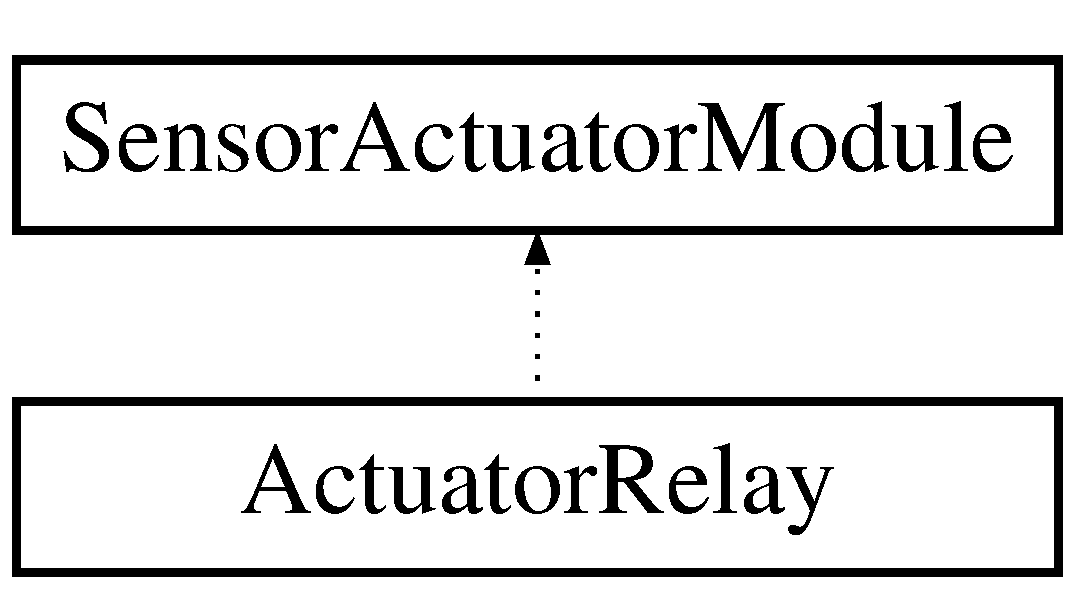
\includegraphics[height=2.000000cm]{class_actuator_relay}
\end{center}
\end{figure}
\subsection*{Public Member Functions}
\begin{DoxyCompactItemize}
\item 
\hyperlink{class_actuator_relay_a0a19fabbd9a3ee500d906a55579ae4f3}{Actuator\+Relay} (int pin, String instruction\+\_\+code, int instruction\+\_\+id)
\begin{DoxyCompactList}\small\item\em Used to construct an instance of the \hyperlink{class_actuator_relay}{Actuator\+Relay} class. \end{DoxyCompactList}\item 
void \hyperlink{class_actuator_relay_abd921e88bb8fcecfbd5e1213e1faad56}{begin} (void)
\begin{DoxyCompactList}\small\item\em Called once to setup module. Sets specified control pin to be in O\+U\+T\+P\+U\+T mode. \end{DoxyCompactList}\item 
String \hyperlink{class_actuator_relay_affbcfa491c42a0aae3d69450cf7295b1}{get} (void)
\begin{DoxyCompactList}\small\item\em Returns J\+S\+O\+N string with module data. Data\+: \char`\"{}$<$instruction\+\_\+code$>$ $<$instruction\+\_\+id$>$ $<$value$>$\char`\"{}, Example\+: \char`\"{}\+A\+A\+H\+U 1 1\char`\"{},. \end{DoxyCompactList}\item 
String \hyperlink{class_actuator_relay_a29995263e5a05a3fdff0761cb4730306}{set} (String instruction\+\_\+code, int instruction\+\_\+id, String instruction\+\_\+parameter)
\begin{DoxyCompactList}\small\item\em Sets relay to be on / off. If instruction\+\_\+code \& instruction\+\_\+id match the code and id module was instantiated with, the relay will enter the state passed in through instruction\+\_\+parameter. If instruction\+\_\+parameter = \char`\"{}1\char`\"{}, relay is O\+N (switch closed). If instruction\+\_\+paremerter = \char`\"{}0\char`\"{}, relay is O\+F\+F (switch open). \end{DoxyCompactList}\end{DoxyCompactItemize}
\subsection*{Public Attributes}
\begin{DoxyCompactItemize}
\item 
int \hyperlink{class_actuator_relay_a8f63c9df6e8dfc90425838f6c1c8fb0e}{value\+\_\+}
\end{DoxyCompactItemize}


\subsection{Detailed Description}
Actuator module for an active low S\+P\+S\+T-\/\+N\+O relay. 

\subsection{Constructor \& Destructor Documentation}
\hypertarget{class_actuator_relay_a0a19fabbd9a3ee500d906a55579ae4f3}{}\index{Actuator\+Relay@{Actuator\+Relay}!Actuator\+Relay@{Actuator\+Relay}}
\index{Actuator\+Relay@{Actuator\+Relay}!Actuator\+Relay@{Actuator\+Relay}}
\subsubsection[{Actuator\+Relay}]{\setlength{\rightskip}{0pt plus 5cm}Actuator\+Relay\+::\+Actuator\+Relay (
\begin{DoxyParamCaption}
\item[{int}]{pin, }
\item[{String}]{instruction\+\_\+code, }
\item[{int}]{instruction\+\_\+id}
\end{DoxyParamCaption}
)}\label{class_actuator_relay_a0a19fabbd9a3ee500d906a55579ae4f3}


Used to construct an instance of the \hyperlink{class_actuator_relay}{Actuator\+Relay} class. 


\begin{DoxyParams}[1]{Parameters}
\mbox{\tt in}  & {\em pin} & is the control line for the relay \\
\hline
\mbox{\tt in}  & {\em instruction\+\_\+code} & is the 4-\/letter instruction code associated with the actuation the relay is switching. \hyperlink{struct_instruction}{Instruction} codes are not necessarily unique. \\
\hline
\mbox{\tt in}  & {\em instruction\+\_\+id} & is the I\+D associated with the specific actuator that is being switched. Each I\+D is unique.\\
\hline
\end{DoxyParams}
To clarify how parameters are used, consider the following case. Imagine there are two air heaters each connected to their own relay. They would have the same instruction code\+: A\+A\+H\+E (Actuator Air Heater) but would both need to be addressable. Thus the instruction\+\_\+ids of the heaters would be 1 and 2. 

\subsection{Member Function Documentation}
\hypertarget{class_actuator_relay_abd921e88bb8fcecfbd5e1213e1faad56}{}\index{Actuator\+Relay@{Actuator\+Relay}!begin@{begin}}
\index{begin@{begin}!Actuator\+Relay@{Actuator\+Relay}}
\subsubsection[{begin}]{\setlength{\rightskip}{0pt plus 5cm}void Actuator\+Relay\+::begin (
\begin{DoxyParamCaption}
\item[{void}]{}
\end{DoxyParamCaption}
)\hspace{0.3cm}{\ttfamily [virtual]}}\label{class_actuator_relay_abd921e88bb8fcecfbd5e1213e1faad56}


Called once to setup module. Sets specified control pin to be in O\+U\+T\+P\+U\+T mode. 



Implements \hyperlink{class_sensor_actuator_module_a453094bcf7c7a2fdb2a14f65bf18bff9}{Sensor\+Actuator\+Module}.

\hypertarget{class_actuator_relay_affbcfa491c42a0aae3d69450cf7295b1}{}\index{Actuator\+Relay@{Actuator\+Relay}!get@{get}}
\index{get@{get}!Actuator\+Relay@{Actuator\+Relay}}
\subsubsection[{get}]{\setlength{\rightskip}{0pt plus 5cm}String Actuator\+Relay\+::get (
\begin{DoxyParamCaption}
\item[{void}]{}
\end{DoxyParamCaption}
)\hspace{0.3cm}{\ttfamily [virtual]}}\label{class_actuator_relay_affbcfa491c42a0aae3d69450cf7295b1}


Returns J\+S\+O\+N string with module data. Data\+: \char`\"{}$<$instruction\+\_\+code$>$ $<$instruction\+\_\+id$>$ $<$value$>$\char`\"{}, Example\+: \char`\"{}\+A\+A\+H\+U 1 1\char`\"{},. 



Implements \hyperlink{class_sensor_actuator_module_a55ce31fe50fc64f90602f3f70c5dc1af}{Sensor\+Actuator\+Module}.

\hypertarget{class_actuator_relay_a29995263e5a05a3fdff0761cb4730306}{}\index{Actuator\+Relay@{Actuator\+Relay}!set@{set}}
\index{set@{set}!Actuator\+Relay@{Actuator\+Relay}}
\subsubsection[{set}]{\setlength{\rightskip}{0pt plus 5cm}String Actuator\+Relay\+::set (
\begin{DoxyParamCaption}
\item[{String}]{instruction\+\_\+code, }
\item[{int}]{instruction\+\_\+id, }
\item[{String}]{instruction\+\_\+parameter}
\end{DoxyParamCaption}
)\hspace{0.3cm}{\ttfamily [virtual]}}\label{class_actuator_relay_a29995263e5a05a3fdff0761cb4730306}


Sets relay to be on / off. If instruction\+\_\+code \& instruction\+\_\+id match the code and id module was instantiated with, the relay will enter the state passed in through instruction\+\_\+parameter. If instruction\+\_\+parameter = \char`\"{}1\char`\"{}, relay is O\+N (switch closed). If instruction\+\_\+paremerter = \char`\"{}0\char`\"{}, relay is O\+F\+F (switch open). 



Implements \hyperlink{class_sensor_actuator_module_adf93ff40fbdfeecbb8711ea0626fe6fc}{Sensor\+Actuator\+Module}.



\subsection{Member Data Documentation}
\hypertarget{class_actuator_relay_a8f63c9df6e8dfc90425838f6c1c8fb0e}{}\index{Actuator\+Relay@{Actuator\+Relay}!value\+\_\+@{value\+\_\+}}
\index{value\+\_\+@{value\+\_\+}!Actuator\+Relay@{Actuator\+Relay}}
\subsubsection[{value\+\_\+}]{\setlength{\rightskip}{0pt plus 5cm}int Actuator\+Relay\+::value\+\_\+}\label{class_actuator_relay_a8f63c9df6e8dfc90425838f6c1c8fb0e}


The documentation for this class was generated from the following files\+:\begin{DoxyCompactItemize}
\item 
src/\hyperlink{actuator__relay_8h}{actuator\+\_\+relay.\+h}\item 
src/\hyperlink{actuator__relay_8cpp}{actuator\+\_\+relay.\+cpp}\end{DoxyCompactItemize}

\hypertarget{class_communication}{}\section{Communication Class Reference}
\label{class_communication}\index{Communication@{Communication}}


Handles a character based serial communication protocol.  




{\ttfamily \#include $<$communication.\+h$>$}

\subsection*{Public Member Functions}
\begin{DoxyCompactItemize}
\item 
void \hyperlink{class_communication_af7eea76d811d38b02fb67ec5133e6eec}{begin} (void)
\item 
void \hyperlink{class_communication_a7905fe8302c11cc1c1dc8a10bc71fdc6}{send} (String message)
\item 
bool \hyperlink{class_communication_a086f2246c7e3715c8de1bc96cfbce262}{available} (void)
\item 
String \hyperlink{class_communication_ad53d6b2efc619612fb542afdfda43ec0}{receive} (void)
\end{DoxyCompactItemize}
\subsection*{Public Attributes}
\begin{DoxyCompactItemize}
\item 
bool \hyperlink{class_communication_a566d648baea3543f997db397e7467a75}{not\+\_\+connected\+\_\+}
\end{DoxyCompactItemize}


\subsection{Detailed Description}
Handles a character based serial communication protocol. 

\subsection{Member Function Documentation}
\hypertarget{class_communication_a086f2246c7e3715c8de1bc96cfbce262}{}\index{Communication@{Communication}!available@{available}}
\index{available@{available}!Communication@{Communication}}
\subsubsection[{available}]{\setlength{\rightskip}{0pt plus 5cm}bool Communication\+::available (
\begin{DoxyParamCaption}
\item[{void}]{}
\end{DoxyParamCaption}
)}\label{class_communication_a086f2246c7e3715c8de1bc96cfbce262}
\hypertarget{class_communication_af7eea76d811d38b02fb67ec5133e6eec}{}\index{Communication@{Communication}!begin@{begin}}
\index{begin@{begin}!Communication@{Communication}}
\subsubsection[{begin}]{\setlength{\rightskip}{0pt plus 5cm}void Communication\+::begin (
\begin{DoxyParamCaption}
\item[{void}]{}
\end{DoxyParamCaption}
)}\label{class_communication_af7eea76d811d38b02fb67ec5133e6eec}
\hypertarget{class_communication_ad53d6b2efc619612fb542afdfda43ec0}{}\index{Communication@{Communication}!receive@{receive}}
\index{receive@{receive}!Communication@{Communication}}
\subsubsection[{receive}]{\setlength{\rightskip}{0pt plus 5cm}String Communication\+::receive (
\begin{DoxyParamCaption}
\item[{void}]{}
\end{DoxyParamCaption}
)}\label{class_communication_ad53d6b2efc619612fb542afdfda43ec0}
\hypertarget{class_communication_a7905fe8302c11cc1c1dc8a10bc71fdc6}{}\index{Communication@{Communication}!send@{send}}
\index{send@{send}!Communication@{Communication}}
\subsubsection[{send}]{\setlength{\rightskip}{0pt plus 5cm}void Communication\+::send (
\begin{DoxyParamCaption}
\item[{String}]{message}
\end{DoxyParamCaption}
)}\label{class_communication_a7905fe8302c11cc1c1dc8a10bc71fdc6}


\subsection{Member Data Documentation}
\hypertarget{class_communication_a566d648baea3543f997db397e7467a75}{}\index{Communication@{Communication}!not\+\_\+connected\+\_\+@{not\+\_\+connected\+\_\+}}
\index{not\+\_\+connected\+\_\+@{not\+\_\+connected\+\_\+}!Communication@{Communication}}
\subsubsection[{not\+\_\+connected\+\_\+}]{\setlength{\rightskip}{0pt plus 5cm}bool Communication\+::not\+\_\+connected\+\_\+}\label{class_communication_a566d648baea3543f997db397e7467a75}


The documentation for this class was generated from the following files\+:\begin{DoxyCompactItemize}
\item 
src/\hyperlink{communication_8h}{communication.\+h}\item 
src/\hyperlink{communication_8cpp}{communication.\+cpp}\end{DoxyCompactItemize}

\hypertarget{struct_instruction}{}\section{Instruction Struct Reference}
\label{struct_instruction}\index{Instruction@{Instruction}}


A structure to represent instruction parameters.  




{\ttfamily \#include $<$module\+\_\+handler.\+h$>$}

\subsection*{Public Attributes}
\begin{DoxyCompactItemize}
\item 
String \hyperlink{struct_instruction_ad888a5bd187437c04dca0f5574ce4ebd}{code}
\item 
int \hyperlink{struct_instruction_aca74587d9d1a44daca3b0965af207a4c}{id}
\item 
String \hyperlink{struct_instruction_a61c139a5e35c88092611020e999e220d}{parameter}
\item 
bool \hyperlink{struct_instruction_a3951b82b53920c98582baa6be7210180}{valid}
\end{DoxyCompactItemize}


\subsection{Detailed Description}
A structure to represent instruction parameters. 


\begin{DoxyParams}{Parameters}
{\em code} & is a 4-\/letter instruction code, not necessarily unique \\
\hline
{\em id} & is the unique I\+D for the instance of the module \\
\hline
{\em parameter} & is the string that contains the message addressed to that specific instruction code and id pair \\
\hline
{\em valid} & indicates whether or not the instruction is valid \\
\hline
\end{DoxyParams}


\subsection{Member Data Documentation}
\hypertarget{struct_instruction_ad888a5bd187437c04dca0f5574ce4ebd}{}\index{Instruction@{Instruction}!code@{code}}
\index{code@{code}!Instruction@{Instruction}}
\subsubsection[{code}]{\setlength{\rightskip}{0pt plus 5cm}String Instruction\+::code}\label{struct_instruction_ad888a5bd187437c04dca0f5574ce4ebd}
\hypertarget{struct_instruction_aca74587d9d1a44daca3b0965af207a4c}{}\index{Instruction@{Instruction}!id@{id}}
\index{id@{id}!Instruction@{Instruction}}
\subsubsection[{id}]{\setlength{\rightskip}{0pt plus 5cm}int Instruction\+::id}\label{struct_instruction_aca74587d9d1a44daca3b0965af207a4c}
\hypertarget{struct_instruction_a61c139a5e35c88092611020e999e220d}{}\index{Instruction@{Instruction}!parameter@{parameter}}
\index{parameter@{parameter}!Instruction@{Instruction}}
\subsubsection[{parameter}]{\setlength{\rightskip}{0pt plus 5cm}String Instruction\+::parameter}\label{struct_instruction_a61c139a5e35c88092611020e999e220d}
\hypertarget{struct_instruction_a3951b82b53920c98582baa6be7210180}{}\index{Instruction@{Instruction}!valid@{valid}}
\index{valid@{valid}!Instruction@{Instruction}}
\subsubsection[{valid}]{\setlength{\rightskip}{0pt plus 5cm}bool Instruction\+::valid}\label{struct_instruction_a3951b82b53920c98582baa6be7210180}


The documentation for this struct was generated from the following file\+:\begin{DoxyCompactItemize}
\item 
src/\hyperlink{module__handler_8h}{module\+\_\+handler.\+h}\end{DoxyCompactItemize}

\hypertarget{class_moving_average_filter}{}\section{Moving\+Average\+Filter Class Reference}
\label{class_moving_average_filter}\index{Moving\+Average\+Filter@{Moving\+Average\+Filter}}


{\ttfamily \#include $<$support\+\_\+moving\+\_\+average.\+h$>$}

\subsection*{Public Member Functions}
\begin{DoxyCompactItemize}
\item 
\hyperlink{class_moving_average_filter_a2845e489c746ffaeb9113e3f87bad8e1}{Moving\+Average\+Filter} (unsigned int new\+Data\+Points\+Count)
\item 
float \hyperlink{class_moving_average_filter_af050822d0acb5a8d32559beb1af0519d}{process} (float in)
\end{DoxyCompactItemize}


\subsection{Constructor \& Destructor Documentation}
\hypertarget{class_moving_average_filter_a2845e489c746ffaeb9113e3f87bad8e1}{}\index{Moving\+Average\+Filter@{Moving\+Average\+Filter}!Moving\+Average\+Filter@{Moving\+Average\+Filter}}
\index{Moving\+Average\+Filter@{Moving\+Average\+Filter}!Moving\+Average\+Filter@{Moving\+Average\+Filter}}
\subsubsection[{Moving\+Average\+Filter}]{\setlength{\rightskip}{0pt plus 5cm}Moving\+Average\+Filter\+::\+Moving\+Average\+Filter (
\begin{DoxyParamCaption}
\item[{unsigned int}]{new\+Data\+Points\+Count}
\end{DoxyParamCaption}
)}\label{class_moving_average_filter_a2845e489c746ffaeb9113e3f87bad8e1}


\subsection{Member Function Documentation}
\hypertarget{class_moving_average_filter_af050822d0acb5a8d32559beb1af0519d}{}\index{Moving\+Average\+Filter@{Moving\+Average\+Filter}!process@{process}}
\index{process@{process}!Moving\+Average\+Filter@{Moving\+Average\+Filter}}
\subsubsection[{process}]{\setlength{\rightskip}{0pt plus 5cm}float Moving\+Average\+Filter\+::process (
\begin{DoxyParamCaption}
\item[{float}]{in}
\end{DoxyParamCaption}
)}\label{class_moving_average_filter_af050822d0acb5a8d32559beb1af0519d}


The documentation for this class was generated from the following files\+:\begin{DoxyCompactItemize}
\item 
src/\hyperlink{support__moving__average_8h}{support\+\_\+moving\+\_\+average.\+h}\item 
src/\hyperlink{support__moving__average_8cpp}{support\+\_\+moving\+\_\+average.\+cpp}\end{DoxyCompactItemize}

\hypertarget{class_one_wire}{}\section{One\+Wire Class Reference}
\label{class_one_wire}\index{One\+Wire@{One\+Wire}}


{\ttfamily \#include $<$support\+\_\+one\+\_\+wire.\+h$>$}

\subsection*{Public Member Functions}
\begin{DoxyCompactItemize}
\item 
\hyperlink{class_one_wire_aa3f23dc51d861a8d257648c507b14e8d}{One\+Wire} (uint8\+\_\+t pin)
\item 
uint8\+\_\+t \hyperlink{class_one_wire_a6a742a9112392567eae3d06dde067c07}{reset} (void)
\item 
void \hyperlink{class_one_wire_accf808390abd63d3c7bce35677784384}{select} (const uint8\+\_\+t rom\mbox{[}8\mbox{]})
\item 
void \hyperlink{class_one_wire_ae3780e2b0ea2ebf6be88298412ac7798}{skip} (void)
\item 
void \hyperlink{class_one_wire_a843e9e7e57ed615b4880be0b76b40b7d}{write} (uint8\+\_\+t v, uint8\+\_\+t power=0)
\item 
void \hyperlink{class_one_wire_a0fc1e0bdc2ab1f062c98567fa60a69ae}{write\+\_\+bytes} (const uint8\+\_\+t $\ast$buf, uint16\+\_\+t count, bool power=0)
\item 
uint8\+\_\+t \hyperlink{class_one_wire_afd9bdb8b5a5b69b394dfc76352e00e21}{read} (void)
\item 
void \hyperlink{class_one_wire_a2407440e8e25b624617593f8ad6447d4}{read\+\_\+bytes} (uint8\+\_\+t $\ast$buf, uint16\+\_\+t count)
\item 
void \hyperlink{class_one_wire_a6bbc58276d1cb08653dab3ea35378f94}{write\+\_\+bit} (uint8\+\_\+t v)
\item 
uint8\+\_\+t \hyperlink{class_one_wire_aeae4c2798b70d9d0ba3091c03ee2d056}{read\+\_\+bit} (void)
\item 
void \hyperlink{class_one_wire_aa8e0f62e830ad05d8035e55c7a309256}{depower} (void)
\item 
void \hyperlink{class_one_wire_aae5efdf67928b5ee312ab7d7906416fa}{reset\+\_\+search} ()
\item 
void \hyperlink{class_one_wire_a0a1b8457adb609a693b865dd474e5116}{target\+\_\+search} (uint8\+\_\+t family\+\_\+code)
\item 
uint8\+\_\+t \hyperlink{class_one_wire_a383dc74fc9f8a27b76366a2859c3820a}{search} (uint8\+\_\+t $\ast$new\+Addr)
\end{DoxyCompactItemize}
\subsection*{Static Public Member Functions}
\begin{DoxyCompactItemize}
\item 
static uint8\+\_\+t \hyperlink{class_one_wire_ae3486a669581b750e4fdf3f3a12b05f1}{crc8} (const uint8\+\_\+t $\ast$addr, uint8\+\_\+t len)
\item 
static bool \hyperlink{class_one_wire_a089c502d26caca5214264261db82d011}{check\+\_\+crc16} (const uint8\+\_\+t $\ast$input, uint16\+\_\+t len, const uint8\+\_\+t $\ast$inverted\+\_\+crc, uint16\+\_\+t crc=0)
\item 
static uint16\+\_\+t \hyperlink{class_one_wire_a685131803ff9bd250926de68fb477998}{crc16} (const uint8\+\_\+t $\ast$input, uint16\+\_\+t len, uint16\+\_\+t crc=0)
\end{DoxyCompactItemize}


\subsection{Constructor \& Destructor Documentation}
\hypertarget{class_one_wire_aa3f23dc51d861a8d257648c507b14e8d}{}\index{One\+Wire@{One\+Wire}!One\+Wire@{One\+Wire}}
\index{One\+Wire@{One\+Wire}!One\+Wire@{One\+Wire}}
\subsubsection[{One\+Wire}]{\setlength{\rightskip}{0pt plus 5cm}One\+Wire\+::\+One\+Wire (
\begin{DoxyParamCaption}
\item[{uint8\+\_\+t}]{pin}
\end{DoxyParamCaption}
)}\label{class_one_wire_aa3f23dc51d861a8d257648c507b14e8d}


\subsection{Member Function Documentation}
\hypertarget{class_one_wire_a089c502d26caca5214264261db82d011}{}\index{One\+Wire@{One\+Wire}!check\+\_\+crc16@{check\+\_\+crc16}}
\index{check\+\_\+crc16@{check\+\_\+crc16}!One\+Wire@{One\+Wire}}
\subsubsection[{check\+\_\+crc16}]{\setlength{\rightskip}{0pt plus 5cm}bool One\+Wire\+::check\+\_\+crc16 (
\begin{DoxyParamCaption}
\item[{const uint8\+\_\+t $\ast$}]{input, }
\item[{uint16\+\_\+t}]{len, }
\item[{const uint8\+\_\+t $\ast$}]{inverted\+\_\+crc, }
\item[{uint16\+\_\+t}]{crc = {\ttfamily 0}}
\end{DoxyParamCaption}
)\hspace{0.3cm}{\ttfamily [static]}}\label{class_one_wire_a089c502d26caca5214264261db82d011}
\hypertarget{class_one_wire_a685131803ff9bd250926de68fb477998}{}\index{One\+Wire@{One\+Wire}!crc16@{crc16}}
\index{crc16@{crc16}!One\+Wire@{One\+Wire}}
\subsubsection[{crc16}]{\setlength{\rightskip}{0pt plus 5cm}uint16\+\_\+t One\+Wire\+::crc16 (
\begin{DoxyParamCaption}
\item[{const uint8\+\_\+t $\ast$}]{input, }
\item[{uint16\+\_\+t}]{len, }
\item[{uint16\+\_\+t}]{crc = {\ttfamily 0}}
\end{DoxyParamCaption}
)\hspace{0.3cm}{\ttfamily [static]}}\label{class_one_wire_a685131803ff9bd250926de68fb477998}
\hypertarget{class_one_wire_ae3486a669581b750e4fdf3f3a12b05f1}{}\index{One\+Wire@{One\+Wire}!crc8@{crc8}}
\index{crc8@{crc8}!One\+Wire@{One\+Wire}}
\subsubsection[{crc8}]{\setlength{\rightskip}{0pt plus 5cm}uint8\+\_\+t One\+Wire\+::crc8 (
\begin{DoxyParamCaption}
\item[{const uint8\+\_\+t $\ast$}]{addr, }
\item[{uint8\+\_\+t}]{len}
\end{DoxyParamCaption}
)\hspace{0.3cm}{\ttfamily [static]}}\label{class_one_wire_ae3486a669581b750e4fdf3f3a12b05f1}
\hypertarget{class_one_wire_aa8e0f62e830ad05d8035e55c7a309256}{}\index{One\+Wire@{One\+Wire}!depower@{depower}}
\index{depower@{depower}!One\+Wire@{One\+Wire}}
\subsubsection[{depower}]{\setlength{\rightskip}{0pt plus 5cm}void One\+Wire\+::depower (
\begin{DoxyParamCaption}
\item[{void}]{}
\end{DoxyParamCaption}
)}\label{class_one_wire_aa8e0f62e830ad05d8035e55c7a309256}
\hypertarget{class_one_wire_afd9bdb8b5a5b69b394dfc76352e00e21}{}\index{One\+Wire@{One\+Wire}!read@{read}}
\index{read@{read}!One\+Wire@{One\+Wire}}
\subsubsection[{read}]{\setlength{\rightskip}{0pt plus 5cm}uint8\+\_\+t One\+Wire\+::read (
\begin{DoxyParamCaption}
\item[{void}]{}
\end{DoxyParamCaption}
)}\label{class_one_wire_afd9bdb8b5a5b69b394dfc76352e00e21}
\hypertarget{class_one_wire_aeae4c2798b70d9d0ba3091c03ee2d056}{}\index{One\+Wire@{One\+Wire}!read\+\_\+bit@{read\+\_\+bit}}
\index{read\+\_\+bit@{read\+\_\+bit}!One\+Wire@{One\+Wire}}
\subsubsection[{read\+\_\+bit}]{\setlength{\rightskip}{0pt plus 5cm}uint8\+\_\+t One\+Wire\+::read\+\_\+bit (
\begin{DoxyParamCaption}
\item[{void}]{}
\end{DoxyParamCaption}
)}\label{class_one_wire_aeae4c2798b70d9d0ba3091c03ee2d056}
\hypertarget{class_one_wire_a2407440e8e25b624617593f8ad6447d4}{}\index{One\+Wire@{One\+Wire}!read\+\_\+bytes@{read\+\_\+bytes}}
\index{read\+\_\+bytes@{read\+\_\+bytes}!One\+Wire@{One\+Wire}}
\subsubsection[{read\+\_\+bytes}]{\setlength{\rightskip}{0pt plus 5cm}void One\+Wire\+::read\+\_\+bytes (
\begin{DoxyParamCaption}
\item[{uint8\+\_\+t $\ast$}]{buf, }
\item[{uint16\+\_\+t}]{count}
\end{DoxyParamCaption}
)}\label{class_one_wire_a2407440e8e25b624617593f8ad6447d4}
\hypertarget{class_one_wire_a6a742a9112392567eae3d06dde067c07}{}\index{One\+Wire@{One\+Wire}!reset@{reset}}
\index{reset@{reset}!One\+Wire@{One\+Wire}}
\subsubsection[{reset}]{\setlength{\rightskip}{0pt plus 5cm}uint8\+\_\+t One\+Wire\+::reset (
\begin{DoxyParamCaption}
\item[{void}]{}
\end{DoxyParamCaption}
)}\label{class_one_wire_a6a742a9112392567eae3d06dde067c07}
\hypertarget{class_one_wire_aae5efdf67928b5ee312ab7d7906416fa}{}\index{One\+Wire@{One\+Wire}!reset\+\_\+search@{reset\+\_\+search}}
\index{reset\+\_\+search@{reset\+\_\+search}!One\+Wire@{One\+Wire}}
\subsubsection[{reset\+\_\+search}]{\setlength{\rightskip}{0pt plus 5cm}void One\+Wire\+::reset\+\_\+search (
\begin{DoxyParamCaption}
{}
\end{DoxyParamCaption}
)}\label{class_one_wire_aae5efdf67928b5ee312ab7d7906416fa}
\hypertarget{class_one_wire_a383dc74fc9f8a27b76366a2859c3820a}{}\index{One\+Wire@{One\+Wire}!search@{search}}
\index{search@{search}!One\+Wire@{One\+Wire}}
\subsubsection[{search}]{\setlength{\rightskip}{0pt plus 5cm}uint8\+\_\+t One\+Wire\+::search (
\begin{DoxyParamCaption}
\item[{uint8\+\_\+t $\ast$}]{new\+Addr}
\end{DoxyParamCaption}
)}\label{class_one_wire_a383dc74fc9f8a27b76366a2859c3820a}
\hypertarget{class_one_wire_accf808390abd63d3c7bce35677784384}{}\index{One\+Wire@{One\+Wire}!select@{select}}
\index{select@{select}!One\+Wire@{One\+Wire}}
\subsubsection[{select}]{\setlength{\rightskip}{0pt plus 5cm}void One\+Wire\+::select (
\begin{DoxyParamCaption}
\item[{const uint8\+\_\+t}]{rom\mbox{[}8\mbox{]}}
\end{DoxyParamCaption}
)}\label{class_one_wire_accf808390abd63d3c7bce35677784384}
\hypertarget{class_one_wire_ae3780e2b0ea2ebf6be88298412ac7798}{}\index{One\+Wire@{One\+Wire}!skip@{skip}}
\index{skip@{skip}!One\+Wire@{One\+Wire}}
\subsubsection[{skip}]{\setlength{\rightskip}{0pt plus 5cm}void One\+Wire\+::skip (
\begin{DoxyParamCaption}
\item[{void}]{}
\end{DoxyParamCaption}
)}\label{class_one_wire_ae3780e2b0ea2ebf6be88298412ac7798}
\hypertarget{class_one_wire_a0a1b8457adb609a693b865dd474e5116}{}\index{One\+Wire@{One\+Wire}!target\+\_\+search@{target\+\_\+search}}
\index{target\+\_\+search@{target\+\_\+search}!One\+Wire@{One\+Wire}}
\subsubsection[{target\+\_\+search}]{\setlength{\rightskip}{0pt plus 5cm}void One\+Wire\+::target\+\_\+search (
\begin{DoxyParamCaption}
\item[{uint8\+\_\+t}]{family\+\_\+code}
\end{DoxyParamCaption}
)}\label{class_one_wire_a0a1b8457adb609a693b865dd474e5116}
\hypertarget{class_one_wire_a843e9e7e57ed615b4880be0b76b40b7d}{}\index{One\+Wire@{One\+Wire}!write@{write}}
\index{write@{write}!One\+Wire@{One\+Wire}}
\subsubsection[{write}]{\setlength{\rightskip}{0pt plus 5cm}void One\+Wire\+::write (
\begin{DoxyParamCaption}
\item[{uint8\+\_\+t}]{v, }
\item[{uint8\+\_\+t}]{power = {\ttfamily 0}}
\end{DoxyParamCaption}
)}\label{class_one_wire_a843e9e7e57ed615b4880be0b76b40b7d}
\hypertarget{class_one_wire_a6bbc58276d1cb08653dab3ea35378f94}{}\index{One\+Wire@{One\+Wire}!write\+\_\+bit@{write\+\_\+bit}}
\index{write\+\_\+bit@{write\+\_\+bit}!One\+Wire@{One\+Wire}}
\subsubsection[{write\+\_\+bit}]{\setlength{\rightskip}{0pt plus 5cm}void One\+Wire\+::write\+\_\+bit (
\begin{DoxyParamCaption}
\item[{uint8\+\_\+t}]{v}
\end{DoxyParamCaption}
)}\label{class_one_wire_a6bbc58276d1cb08653dab3ea35378f94}
\hypertarget{class_one_wire_a0fc1e0bdc2ab1f062c98567fa60a69ae}{}\index{One\+Wire@{One\+Wire}!write\+\_\+bytes@{write\+\_\+bytes}}
\index{write\+\_\+bytes@{write\+\_\+bytes}!One\+Wire@{One\+Wire}}
\subsubsection[{write\+\_\+bytes}]{\setlength{\rightskip}{0pt plus 5cm}void One\+Wire\+::write\+\_\+bytes (
\begin{DoxyParamCaption}
\item[{const uint8\+\_\+t $\ast$}]{buf, }
\item[{uint16\+\_\+t}]{count, }
\item[{bool}]{power = {\ttfamily 0}}
\end{DoxyParamCaption}
)}\label{class_one_wire_a0fc1e0bdc2ab1f062c98567fa60a69ae}


The documentation for this class was generated from the following files\+:\begin{DoxyCompactItemize}
\item 
src/\hyperlink{support__one__wire_8h}{support\+\_\+one\+\_\+wire.\+h}\item 
src/\hyperlink{support__one__wire_8cpp}{support\+\_\+one\+\_\+wire.\+cpp}\end{DoxyCompactItemize}

\hypertarget{class_sensor_actuator_module}{}\section{Sensor\+Actuator\+Module Class Reference}
\label{class_sensor_actuator_module}\index{Sensor\+Actuator\+Module@{Sensor\+Actuator\+Module}}


Abstract class used as the interface for all Sensor Actuator Modules.  




{\ttfamily \#include $<$module\+\_\+handler.\+h$>$}

Inheritance diagram for Sensor\+Actuator\+Module\+:\begin{figure}[H]
\begin{center}
\leavevmode
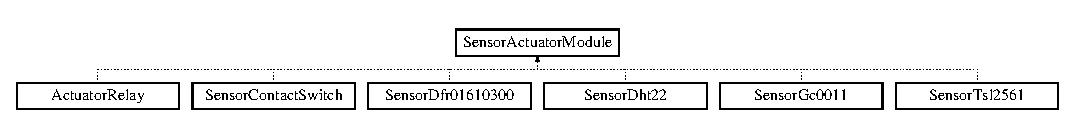
\includegraphics[height=1.244444cm]{class_sensor_actuator_module}
\end{center}
\end{figure}
\subsection*{Public Member Functions}
\begin{DoxyCompactItemize}
\item 
virtual void \hyperlink{class_sensor_actuator_module_a453094bcf7c7a2fdb2a14f65bf18bff9}{begin} (void)=0
\begin{DoxyCompactList}\small\item\em Called once at beginning of program to initialize modules. \end{DoxyCompactList}\item 
virtual String \hyperlink{class_sensor_actuator_module_a55ce31fe50fc64f90602f3f70c5dc1af}{get} (void)=0
\begin{DoxyCompactList}\small\item\em Called once per loop iteration to update and report module data to controller. \end{DoxyCompactList}\item 
virtual String \hyperlink{class_sensor_actuator_module_adf93ff40fbdfeecbb8711ea0626fe6fc}{set} (String instruction\+\_\+code, int instruction\+\_\+id, String instruction\+\_\+parameter)=0
\begin{DoxyCompactList}\small\item\em Called once per loop iteration to update module state. If response is generated from updating, reports response to controller. \end{DoxyCompactList}\end{DoxyCompactItemize}


\subsection{Detailed Description}
Abstract class used as the interface for all Sensor Actuator Modules. 

\subsection{Member Function Documentation}
\hypertarget{class_sensor_actuator_module_a453094bcf7c7a2fdb2a14f65bf18bff9}{}\index{Sensor\+Actuator\+Module@{Sensor\+Actuator\+Module}!begin@{begin}}
\index{begin@{begin}!Sensor\+Actuator\+Module@{Sensor\+Actuator\+Module}}
\subsubsection[{begin}]{\setlength{\rightskip}{0pt plus 5cm}virtual void Sensor\+Actuator\+Module\+::begin (
\begin{DoxyParamCaption}
\item[{void}]{}
\end{DoxyParamCaption}
)\hspace{0.3cm}{\ttfamily [pure virtual]}}\label{class_sensor_actuator_module_a453094bcf7c7a2fdb2a14f65bf18bff9}


Called once at beginning of program to initialize modules. 



Implemented in \hyperlink{class_sensor_tsl2561_ace17c892222366185df021bda708cc10}{Sensor\+Tsl2561}, \hyperlink{class_sensor_dfr01610300_a456221ff4728d8985c8e980d4f22b692}{Sensor\+Dfr01610300}, \hyperlink{class_actuator_relay_abd921e88bb8fcecfbd5e1213e1faad56}{Actuator\+Relay}, \hyperlink{class_sensor_dht22_ae4de2976d82d060c9dc12bf84195a347}{Sensor\+Dht22}, \hyperlink{class_sensor_gc0011_a661743d47448c6b9c965fd8e1f123fbc}{Sensor\+Gc0011}, and \hyperlink{class_sensor_contact_switch_a037d866b1e40776cc6fa00a46169b150}{Sensor\+Contact\+Switch}.

\hypertarget{class_sensor_actuator_module_a55ce31fe50fc64f90602f3f70c5dc1af}{}\index{Sensor\+Actuator\+Module@{Sensor\+Actuator\+Module}!get@{get}}
\index{get@{get}!Sensor\+Actuator\+Module@{Sensor\+Actuator\+Module}}
\subsubsection[{get}]{\setlength{\rightskip}{0pt plus 5cm}virtual String Sensor\+Actuator\+Module\+::get (
\begin{DoxyParamCaption}
\item[{void}]{}
\end{DoxyParamCaption}
)\hspace{0.3cm}{\ttfamily [pure virtual]}}\label{class_sensor_actuator_module_a55ce31fe50fc64f90602f3f70c5dc1af}


Called once per loop iteration to update and report module data to controller. 



Implemented in \hyperlink{class_sensor_tsl2561_a1d9dff52af755218abca50f9025f0f5c}{Sensor\+Tsl2561}, \hyperlink{class_sensor_dfr01610300_a21bbd0f8ee7e6576eabd9acf0e1e4d89}{Sensor\+Dfr01610300}, \hyperlink{class_actuator_relay_affbcfa491c42a0aae3d69450cf7295b1}{Actuator\+Relay}, \hyperlink{class_sensor_dht22_ad939eefeb967eea7029d9505cc6aad6f}{Sensor\+Dht22}, \hyperlink{class_sensor_gc0011_a2920401f54e121bba1398d52e9b2c90a}{Sensor\+Gc0011}, and \hyperlink{class_sensor_contact_switch_a99a5906b45ed441eea56fb2960d35191}{Sensor\+Contact\+Switch}.

\hypertarget{class_sensor_actuator_module_adf93ff40fbdfeecbb8711ea0626fe6fc}{}\index{Sensor\+Actuator\+Module@{Sensor\+Actuator\+Module}!set@{set}}
\index{set@{set}!Sensor\+Actuator\+Module@{Sensor\+Actuator\+Module}}
\subsubsection[{set}]{\setlength{\rightskip}{0pt plus 5cm}virtual String Sensor\+Actuator\+Module\+::set (
\begin{DoxyParamCaption}
\item[{String}]{instruction\+\_\+code, }
\item[{int}]{instruction\+\_\+id, }
\item[{String}]{instruction\+\_\+parameter}
\end{DoxyParamCaption}
)\hspace{0.3cm}{\ttfamily [pure virtual]}}\label{class_sensor_actuator_module_adf93ff40fbdfeecbb8711ea0626fe6fc}


Called once per loop iteration to update module state. If response is generated from updating, reports response to controller. 



Implemented in \hyperlink{class_sensor_tsl2561_ab4eb3d8197c96867f43857876df46b33}{Sensor\+Tsl2561}, \hyperlink{class_sensor_dfr01610300_ab675c2708ff9d5d0d9bbe10bab3d97e8}{Sensor\+Dfr01610300}, \hyperlink{class_actuator_relay_a29995263e5a05a3fdff0761cb4730306}{Actuator\+Relay}, \hyperlink{class_sensor_dht22_a177a42edbc33d5cf4fa0c4c38dc0047c}{Sensor\+Dht22}, \hyperlink{class_sensor_gc0011_a658b7856221577342b54e4dc7fe06d2a}{Sensor\+Gc0011}, and \hyperlink{class_sensor_contact_switch_ab49acd5d6132eed50d7342717649abc2}{Sensor\+Contact\+Switch}.



The documentation for this class was generated from the following file\+:\begin{DoxyCompactItemize}
\item 
src/\hyperlink{module__handler_8h}{module\+\_\+handler.\+h}\end{DoxyCompactItemize}

\hypertarget{class_sensor_contact_switch}{}\section{Sensor\+Contact\+Switch Class Reference}
\label{class_sensor_contact_switch}\index{Sensor\+Contact\+Switch@{Sensor\+Contact\+Switch}}


Sensor module for all sensors that behave like a contact switch.  




{\ttfamily \#include $<$sensor\+\_\+contact\+\_\+switch.\+h$>$}

Inheritance diagram for Sensor\+Contact\+Switch\+:\begin{figure}[H]
\begin{center}
\leavevmode
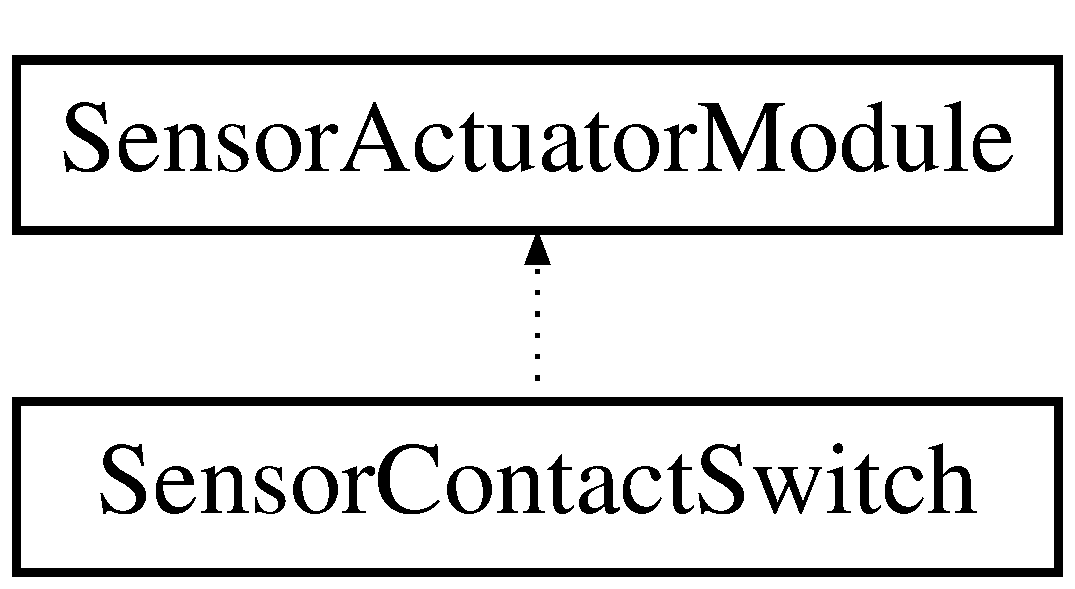
\includegraphics[height=2.000000cm]{class_sensor_contact_switch}
\end{center}
\end{figure}
\subsection*{Public Member Functions}
\begin{DoxyCompactItemize}
\item 
\hyperlink{class_sensor_contact_switch_a821878d797ea7b94dd2870f98df8fdf5}{Sensor\+Contact\+Switch} (int pin, String instruction\+\_\+code, int instruction\+\_\+id)
\item 
void \hyperlink{class_sensor_contact_switch_a037d866b1e40776cc6fa00a46169b150}{begin} (void)
\begin{DoxyCompactList}\small\item\em Called once at beginning of program to initialize modules. \end{DoxyCompactList}\item 
String \hyperlink{class_sensor_contact_switch_a99a5906b45ed441eea56fb2960d35191}{get} (void)
\begin{DoxyCompactList}\small\item\em Called once per loop iteration to update and report module data to controller. \end{DoxyCompactList}\item 
String \hyperlink{class_sensor_contact_switch_ab49acd5d6132eed50d7342717649abc2}{set} (String instruction\+\_\+code, int instruction\+\_\+id, String instruction\+\_\+parameter)
\begin{DoxyCompactList}\small\item\em Called once per loop iteration to update module state. If response is generated from updating, reports response to controller. \end{DoxyCompactList}\end{DoxyCompactItemize}
\subsection*{Public Attributes}
\begin{DoxyCompactItemize}
\item 
bool \hyperlink{class_sensor_contact_switch_a38d5bad22015b2013e776dec61bc8622}{is\+\_\+connected\+\_\+}
\end{DoxyCompactItemize}


\subsection{Detailed Description}
Sensor module for all sensors that behave like a contact switch. 

\subsection{Constructor \& Destructor Documentation}
\hypertarget{class_sensor_contact_switch_a821878d797ea7b94dd2870f98df8fdf5}{}\index{Sensor\+Contact\+Switch@{Sensor\+Contact\+Switch}!Sensor\+Contact\+Switch@{Sensor\+Contact\+Switch}}
\index{Sensor\+Contact\+Switch@{Sensor\+Contact\+Switch}!Sensor\+Contact\+Switch@{Sensor\+Contact\+Switch}}
\subsubsection[{Sensor\+Contact\+Switch}]{\setlength{\rightskip}{0pt plus 5cm}Sensor\+Contact\+Switch\+::\+Sensor\+Contact\+Switch (
\begin{DoxyParamCaption}
\item[{int}]{pin, }
\item[{String}]{instruction\+\_\+code, }
\item[{int}]{instruction\+\_\+id}
\end{DoxyParamCaption}
)}\label{class_sensor_contact_switch_a821878d797ea7b94dd2870f98df8fdf5}


\subsection{Member Function Documentation}
\hypertarget{class_sensor_contact_switch_a037d866b1e40776cc6fa00a46169b150}{}\index{Sensor\+Contact\+Switch@{Sensor\+Contact\+Switch}!begin@{begin}}
\index{begin@{begin}!Sensor\+Contact\+Switch@{Sensor\+Contact\+Switch}}
\subsubsection[{begin}]{\setlength{\rightskip}{0pt plus 5cm}void Sensor\+Contact\+Switch\+::begin (
\begin{DoxyParamCaption}
\item[{void}]{}
\end{DoxyParamCaption}
)\hspace{0.3cm}{\ttfamily [virtual]}}\label{class_sensor_contact_switch_a037d866b1e40776cc6fa00a46169b150}


Called once at beginning of program to initialize modules. 



Implements \hyperlink{class_sensor_actuator_module_a453094bcf7c7a2fdb2a14f65bf18bff9}{Sensor\+Actuator\+Module}.

\hypertarget{class_sensor_contact_switch_a99a5906b45ed441eea56fb2960d35191}{}\index{Sensor\+Contact\+Switch@{Sensor\+Contact\+Switch}!get@{get}}
\index{get@{get}!Sensor\+Contact\+Switch@{Sensor\+Contact\+Switch}}
\subsubsection[{get}]{\setlength{\rightskip}{0pt plus 5cm}String Sensor\+Contact\+Switch\+::get (
\begin{DoxyParamCaption}
\item[{void}]{}
\end{DoxyParamCaption}
)\hspace{0.3cm}{\ttfamily [virtual]}}\label{class_sensor_contact_switch_a99a5906b45ed441eea56fb2960d35191}


Called once per loop iteration to update and report module data to controller. 



Implements \hyperlink{class_sensor_actuator_module_a55ce31fe50fc64f90602f3f70c5dc1af}{Sensor\+Actuator\+Module}.

\hypertarget{class_sensor_contact_switch_ab49acd5d6132eed50d7342717649abc2}{}\index{Sensor\+Contact\+Switch@{Sensor\+Contact\+Switch}!set@{set}}
\index{set@{set}!Sensor\+Contact\+Switch@{Sensor\+Contact\+Switch}}
\subsubsection[{set}]{\setlength{\rightskip}{0pt plus 5cm}String Sensor\+Contact\+Switch\+::set (
\begin{DoxyParamCaption}
\item[{String}]{instruction\+\_\+code, }
\item[{int}]{instruction\+\_\+id, }
\item[{String}]{instruction\+\_\+parameter}
\end{DoxyParamCaption}
)\hspace{0.3cm}{\ttfamily [virtual]}}\label{class_sensor_contact_switch_ab49acd5d6132eed50d7342717649abc2}


Called once per loop iteration to update module state. If response is generated from updating, reports response to controller. 



Implements \hyperlink{class_sensor_actuator_module_adf93ff40fbdfeecbb8711ea0626fe6fc}{Sensor\+Actuator\+Module}.



\subsection{Member Data Documentation}
\hypertarget{class_sensor_contact_switch_a38d5bad22015b2013e776dec61bc8622}{}\index{Sensor\+Contact\+Switch@{Sensor\+Contact\+Switch}!is\+\_\+connected\+\_\+@{is\+\_\+connected\+\_\+}}
\index{is\+\_\+connected\+\_\+@{is\+\_\+connected\+\_\+}!Sensor\+Contact\+Switch@{Sensor\+Contact\+Switch}}
\subsubsection[{is\+\_\+connected\+\_\+}]{\setlength{\rightskip}{0pt plus 5cm}bool Sensor\+Contact\+Switch\+::is\+\_\+connected\+\_\+}\label{class_sensor_contact_switch_a38d5bad22015b2013e776dec61bc8622}


The documentation for this class was generated from the following files\+:\begin{DoxyCompactItemize}
\item 
src/\hyperlink{sensor__contact__switch_8h}{sensor\+\_\+contact\+\_\+switch.\+h}\item 
src/\hyperlink{sensor__contact__switch_8cpp}{sensor\+\_\+contact\+\_\+switch.\+cpp}\end{DoxyCompactItemize}

\hypertarget{class_sensor_dfr01610300}{}\section{Sensor\+Dfr01610300 Class Reference}
\label{class_sensor_dfr01610300}\index{Sensor\+Dfr01610300@{Sensor\+Dfr01610300}}


Sensor module for water ph, ec, and temperature.  




{\ttfamily \#include $<$sensor\+\_\+dfr0161\+\_\+0300.\+h$>$}

Inheritance diagram for Sensor\+Dfr01610300\+:\begin{figure}[H]
\begin{center}
\leavevmode
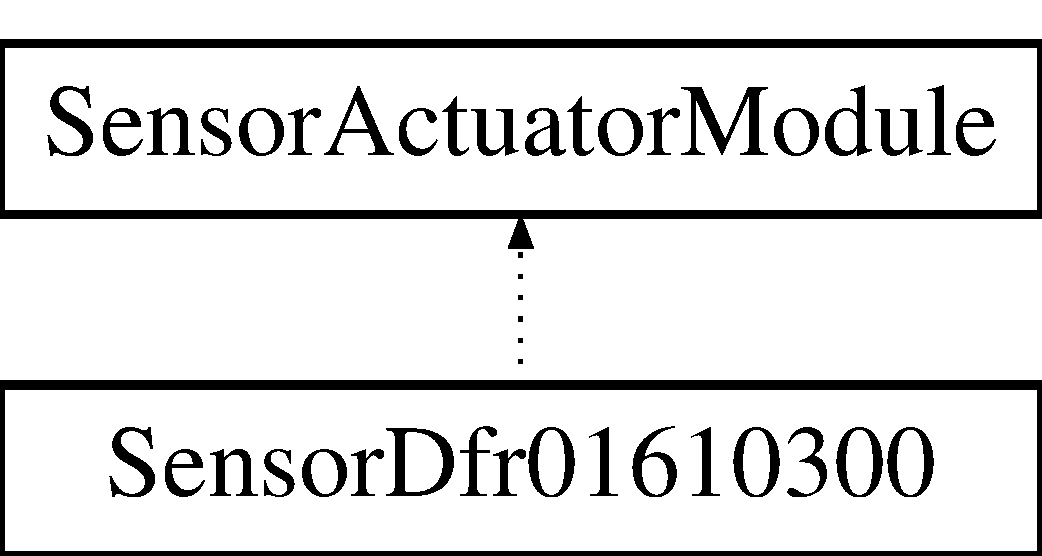
\includegraphics[height=2.000000cm]{class_sensor_dfr01610300}
\end{center}
\end{figure}
\subsection*{Public Member Functions}
\begin{DoxyCompactItemize}
\item 
\hyperlink{class_sensor_dfr01610300_aeb40fef336ad2b2d82f7c5eddf9d318e}{Sensor\+Dfr01610300} (int ph\+\_\+pin, String ph\+\_\+instruction\+\_\+code, int ph\+\_\+instruction\+\_\+id, int temperature\+\_\+pin, String temperature\+\_\+instruction\+\_\+code, int temperature\+\_\+id, int ec\+\_\+pin, String ec\+\_\+instruction\+\_\+code, int ec\+\_\+id, int ec\+\_\+enable\+\_\+pin)
\item 
void \hyperlink{class_sensor_dfr01610300_a456221ff4728d8985c8e980d4f22b692}{begin} (void)
\begin{DoxyCompactList}\small\item\em Called once to setup module. Declares objects, configures initial state, sets configuration \& calibration parameters. \end{DoxyCompactList}\item 
String \hyperlink{class_sensor_dfr01610300_a21bbd0f8ee7e6576eabd9acf0e1e4d89}{get} (void)
\begin{DoxyCompactList}\small\item\em Returns J\+S\+O\+N string with module data. Module data\+: ph, temperature, ec. Data\+: \char`\"{}$<$instruction\+\_\+code$>$ $<$instruction\+\_\+id$>$ $<$value$>$\char`\"{}. Example\+: \char`\"{}\+S\+W\+P\+H 1 1\char`\"{}, \char`\"{}\+S\+W\+T\+M 1 1\char`\"{}, \char`\"{}\+S\+W\+E\+C 1 1\char`\"{},. \end{DoxyCompactList}\item 
String \hyperlink{class_sensor_dfr01610300_ab675c2708ff9d5d0d9bbe10bab3d97e8}{set} (String instruction\+\_\+code, int instruction\+\_\+id, String instruction\+\_\+parameter)
\begin{DoxyCompactList}\small\item\em Reserved to passing data string to object Currently unused. Exists to comply with S\+A\+Module interface. \end{DoxyCompactList}\end{DoxyCompactItemize}
\subsection*{Public Attributes}
\begin{DoxyCompactItemize}
\item 
float \hyperlink{class_sensor_dfr01610300_aa0ab70c745bde253adaa343afba56473}{ph\+\_\+raw}
\item 
float \hyperlink{class_sensor_dfr01610300_a09ae20cb63d44609c717dda168b8e454}{ph\+\_\+filtered}
\item 
float \hyperlink{class_sensor_dfr01610300_a483485c4c8a91569e8f45819e641e38c}{temperature\+\_\+raw}
\item 
float \hyperlink{class_sensor_dfr01610300_a598f2f18f66d626a3ce392478fcadcc8}{temperature\+\_\+filtered}
\item 
float \hyperlink{class_sensor_dfr01610300_af0fc005c44506d277f792acd29f64c3e}{ec\+\_\+raw}
\item 
float \hyperlink{class_sensor_dfr01610300_a3183d77d8012266006113a3d8647a2a9}{ec\+\_\+filtered}
\end{DoxyCompactItemize}


\subsection{Detailed Description}
Sensor module for water ph, ec, and temperature. 

\subsection{Constructor \& Destructor Documentation}
\hypertarget{class_sensor_dfr01610300_aeb40fef336ad2b2d82f7c5eddf9d318e}{}\index{Sensor\+Dfr01610300@{Sensor\+Dfr01610300}!Sensor\+Dfr01610300@{Sensor\+Dfr01610300}}
\index{Sensor\+Dfr01610300@{Sensor\+Dfr01610300}!Sensor\+Dfr01610300@{Sensor\+Dfr01610300}}
\subsubsection[{Sensor\+Dfr01610300}]{\setlength{\rightskip}{0pt plus 5cm}Sensor\+Dfr01610300\+::\+Sensor\+Dfr01610300 (
\begin{DoxyParamCaption}
\item[{int}]{ph\+\_\+pin, }
\item[{String}]{ph\+\_\+instruction\+\_\+code, }
\item[{int}]{ph\+\_\+instruction\+\_\+id, }
\item[{int}]{temperature\+\_\+pin, }
\item[{String}]{temperature\+\_\+instruction\+\_\+code, }
\item[{int}]{temperature\+\_\+id, }
\item[{int}]{ec\+\_\+pin, }
\item[{String}]{ec\+\_\+instruction\+\_\+code, }
\item[{int}]{ec\+\_\+id, }
\item[{int}]{ec\+\_\+enable\+\_\+pin}
\end{DoxyParamCaption}
)}\label{class_sensor_dfr01610300_aeb40fef336ad2b2d82f7c5eddf9d318e}


\subsection{Member Function Documentation}
\hypertarget{class_sensor_dfr01610300_a456221ff4728d8985c8e980d4f22b692}{}\index{Sensor\+Dfr01610300@{Sensor\+Dfr01610300}!begin@{begin}}
\index{begin@{begin}!Sensor\+Dfr01610300@{Sensor\+Dfr01610300}}
\subsubsection[{begin}]{\setlength{\rightskip}{0pt plus 5cm}void Sensor\+Dfr01610300\+::begin (
\begin{DoxyParamCaption}
\item[{void}]{}
\end{DoxyParamCaption}
)\hspace{0.3cm}{\ttfamily [virtual]}}\label{class_sensor_dfr01610300_a456221ff4728d8985c8e980d4f22b692}


Called once to setup module. Declares objects, configures initial state, sets configuration \& calibration parameters. 



Implements \hyperlink{class_sensor_actuator_module_a453094bcf7c7a2fdb2a14f65bf18bff9}{Sensor\+Actuator\+Module}.

\hypertarget{class_sensor_dfr01610300_a21bbd0f8ee7e6576eabd9acf0e1e4d89}{}\index{Sensor\+Dfr01610300@{Sensor\+Dfr01610300}!get@{get}}
\index{get@{get}!Sensor\+Dfr01610300@{Sensor\+Dfr01610300}}
\subsubsection[{get}]{\setlength{\rightskip}{0pt plus 5cm}String Sensor\+Dfr01610300\+::get (
\begin{DoxyParamCaption}
\item[{void}]{}
\end{DoxyParamCaption}
)\hspace{0.3cm}{\ttfamily [virtual]}}\label{class_sensor_dfr01610300_a21bbd0f8ee7e6576eabd9acf0e1e4d89}


Returns J\+S\+O\+N string with module data. Module data\+: ph, temperature, ec. Data\+: \char`\"{}$<$instruction\+\_\+code$>$ $<$instruction\+\_\+id$>$ $<$value$>$\char`\"{}. Example\+: \char`\"{}\+S\+W\+P\+H 1 1\char`\"{}, \char`\"{}\+S\+W\+T\+M 1 1\char`\"{}, \char`\"{}\+S\+W\+E\+C 1 1\char`\"{},. 



Implements \hyperlink{class_sensor_actuator_module_a55ce31fe50fc64f90602f3f70c5dc1af}{Sensor\+Actuator\+Module}.

\hypertarget{class_sensor_dfr01610300_ab675c2708ff9d5d0d9bbe10bab3d97e8}{}\index{Sensor\+Dfr01610300@{Sensor\+Dfr01610300}!set@{set}}
\index{set@{set}!Sensor\+Dfr01610300@{Sensor\+Dfr01610300}}
\subsubsection[{set}]{\setlength{\rightskip}{0pt plus 5cm}String Sensor\+Dfr01610300\+::set (
\begin{DoxyParamCaption}
\item[{String}]{instruction\+\_\+code, }
\item[{int}]{instruction\+\_\+id, }
\item[{String}]{instruction\+\_\+parameter}
\end{DoxyParamCaption}
)\hspace{0.3cm}{\ttfamily [virtual]}}\label{class_sensor_dfr01610300_ab675c2708ff9d5d0d9bbe10bab3d97e8}


Reserved to passing data string to object Currently unused. Exists to comply with S\+A\+Module interface. 



Implements \hyperlink{class_sensor_actuator_module_adf93ff40fbdfeecbb8711ea0626fe6fc}{Sensor\+Actuator\+Module}.



\subsection{Member Data Documentation}
\hypertarget{class_sensor_dfr01610300_a3183d77d8012266006113a3d8647a2a9}{}\index{Sensor\+Dfr01610300@{Sensor\+Dfr01610300}!ec\+\_\+filtered@{ec\+\_\+filtered}}
\index{ec\+\_\+filtered@{ec\+\_\+filtered}!Sensor\+Dfr01610300@{Sensor\+Dfr01610300}}
\subsubsection[{ec\+\_\+filtered}]{\setlength{\rightskip}{0pt plus 5cm}float Sensor\+Dfr01610300\+::ec\+\_\+filtered}\label{class_sensor_dfr01610300_a3183d77d8012266006113a3d8647a2a9}
\hypertarget{class_sensor_dfr01610300_af0fc005c44506d277f792acd29f64c3e}{}\index{Sensor\+Dfr01610300@{Sensor\+Dfr01610300}!ec\+\_\+raw@{ec\+\_\+raw}}
\index{ec\+\_\+raw@{ec\+\_\+raw}!Sensor\+Dfr01610300@{Sensor\+Dfr01610300}}
\subsubsection[{ec\+\_\+raw}]{\setlength{\rightskip}{0pt plus 5cm}float Sensor\+Dfr01610300\+::ec\+\_\+raw}\label{class_sensor_dfr01610300_af0fc005c44506d277f792acd29f64c3e}
\hypertarget{class_sensor_dfr01610300_a09ae20cb63d44609c717dda168b8e454}{}\index{Sensor\+Dfr01610300@{Sensor\+Dfr01610300}!ph\+\_\+filtered@{ph\+\_\+filtered}}
\index{ph\+\_\+filtered@{ph\+\_\+filtered}!Sensor\+Dfr01610300@{Sensor\+Dfr01610300}}
\subsubsection[{ph\+\_\+filtered}]{\setlength{\rightskip}{0pt plus 5cm}float Sensor\+Dfr01610300\+::ph\+\_\+filtered}\label{class_sensor_dfr01610300_a09ae20cb63d44609c717dda168b8e454}
\hypertarget{class_sensor_dfr01610300_aa0ab70c745bde253adaa343afba56473}{}\index{Sensor\+Dfr01610300@{Sensor\+Dfr01610300}!ph\+\_\+raw@{ph\+\_\+raw}}
\index{ph\+\_\+raw@{ph\+\_\+raw}!Sensor\+Dfr01610300@{Sensor\+Dfr01610300}}
\subsubsection[{ph\+\_\+raw}]{\setlength{\rightskip}{0pt plus 5cm}float Sensor\+Dfr01610300\+::ph\+\_\+raw}\label{class_sensor_dfr01610300_aa0ab70c745bde253adaa343afba56473}
\hypertarget{class_sensor_dfr01610300_a598f2f18f66d626a3ce392478fcadcc8}{}\index{Sensor\+Dfr01610300@{Sensor\+Dfr01610300}!temperature\+\_\+filtered@{temperature\+\_\+filtered}}
\index{temperature\+\_\+filtered@{temperature\+\_\+filtered}!Sensor\+Dfr01610300@{Sensor\+Dfr01610300}}
\subsubsection[{temperature\+\_\+filtered}]{\setlength{\rightskip}{0pt plus 5cm}float Sensor\+Dfr01610300\+::temperature\+\_\+filtered}\label{class_sensor_dfr01610300_a598f2f18f66d626a3ce392478fcadcc8}
\hypertarget{class_sensor_dfr01610300_a483485c4c8a91569e8f45819e641e38c}{}\index{Sensor\+Dfr01610300@{Sensor\+Dfr01610300}!temperature\+\_\+raw@{temperature\+\_\+raw}}
\index{temperature\+\_\+raw@{temperature\+\_\+raw}!Sensor\+Dfr01610300@{Sensor\+Dfr01610300}}
\subsubsection[{temperature\+\_\+raw}]{\setlength{\rightskip}{0pt plus 5cm}float Sensor\+Dfr01610300\+::temperature\+\_\+raw}\label{class_sensor_dfr01610300_a483485c4c8a91569e8f45819e641e38c}


The documentation for this class was generated from the following files\+:\begin{DoxyCompactItemize}
\item 
src/\hyperlink{sensor__dfr0161__0300_8h}{sensor\+\_\+dfr0161\+\_\+0300.\+h}\item 
src/\hyperlink{sensor__dfr0161__0300_8cpp}{sensor\+\_\+dfr0161\+\_\+0300.\+cpp}\end{DoxyCompactItemize}

\hypertarget{class_sensor_dht22}{}\section{Sensor\+Dht22 Class Reference}
\label{class_sensor_dht22}\index{Sensor\+Dht22@{Sensor\+Dht22}}


Sensor module for air temperature and humidity.  




{\ttfamily \#include $<$sensor\+\_\+dht22.\+h$>$}

Inheritance diagram for Sensor\+Dht22\+:\begin{figure}[H]
\begin{center}
\leavevmode
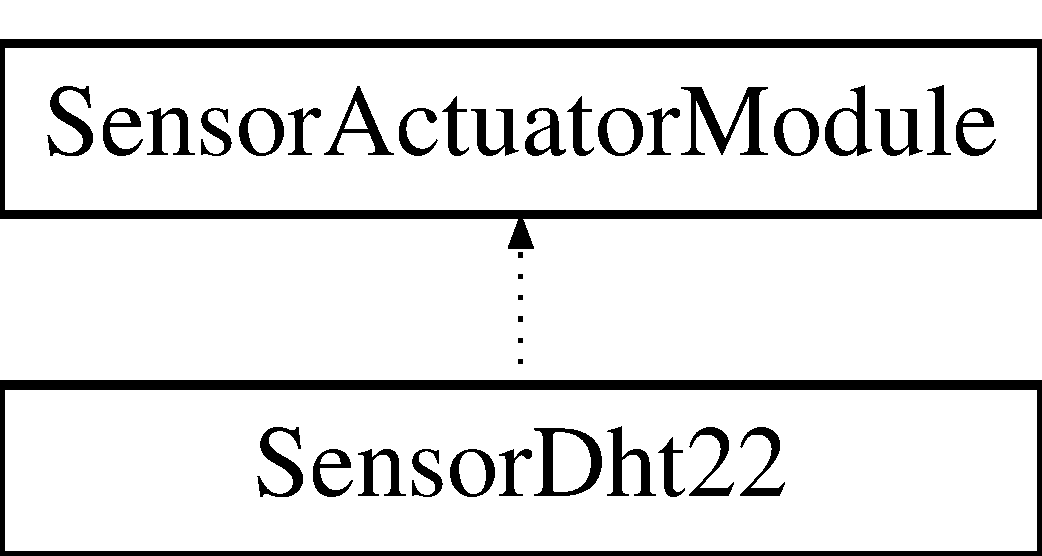
\includegraphics[height=2.000000cm]{class_sensor_dht22}
\end{center}
\end{figure}
\subsection*{Public Member Functions}
\begin{DoxyCompactItemize}
\item 
\hyperlink{class_sensor_dht22_a417840f2a31737059e6b0885d89de32f}{Sensor\+Dht22} (int pin, String temperature\+\_\+instruction\+\_\+code, int temperature\+\_\+instruction\+\_\+id, String humidity\+\_\+instruction\+\_\+code, int humidity\+\_\+instruction\+\_\+id)
\item 
void \hyperlink{class_sensor_dht22_ae4de2976d82d060c9dc12bf84195a347}{begin} (void)
\begin{DoxyCompactList}\small\item\em Called once at beginning of program to initialize modules. \end{DoxyCompactList}\item 
String \hyperlink{class_sensor_dht22_ad939eefeb967eea7029d9505cc6aad6f}{get} (void)
\begin{DoxyCompactList}\small\item\em Called once per loop iteration to update and report module data to controller. \end{DoxyCompactList}\item 
String \hyperlink{class_sensor_dht22_a177a42edbc33d5cf4fa0c4c38dc0047c}{set} (String instruction\+\_\+code, int instruction\+\_\+id, String parameter)
\begin{DoxyCompactList}\small\item\em Called once per loop iteration to update module state. If response is generated from updating, reports response to controller. \end{DoxyCompactList}\end{DoxyCompactItemize}
\subsection*{Public Attributes}
\begin{DoxyCompactItemize}
\item 
float \hyperlink{class_sensor_dht22_a93f9363f3086e00f440fc89a7f1f8a1b}{humidity}
\item 
float \hyperlink{class_sensor_dht22_af35665067c66e887afa5fef5611fb48a}{temperature}
\end{DoxyCompactItemize}


\subsection{Detailed Description}
Sensor module for air temperature and humidity. 

\subsection{Constructor \& Destructor Documentation}
\hypertarget{class_sensor_dht22_a417840f2a31737059e6b0885d89de32f}{}\index{Sensor\+Dht22@{Sensor\+Dht22}!Sensor\+Dht22@{Sensor\+Dht22}}
\index{Sensor\+Dht22@{Sensor\+Dht22}!Sensor\+Dht22@{Sensor\+Dht22}}
\subsubsection[{Sensor\+Dht22}]{\setlength{\rightskip}{0pt plus 5cm}Sensor\+Dht22\+::\+Sensor\+Dht22 (
\begin{DoxyParamCaption}
\item[{int}]{pin, }
\item[{String}]{temperature\+\_\+instruction\+\_\+code, }
\item[{int}]{temperature\+\_\+instruction\+\_\+id, }
\item[{String}]{humidity\+\_\+instruction\+\_\+code, }
\item[{int}]{humidity\+\_\+instruction\+\_\+id}
\end{DoxyParamCaption}
)}\label{class_sensor_dht22_a417840f2a31737059e6b0885d89de32f}


\subsection{Member Function Documentation}
\hypertarget{class_sensor_dht22_ae4de2976d82d060c9dc12bf84195a347}{}\index{Sensor\+Dht22@{Sensor\+Dht22}!begin@{begin}}
\index{begin@{begin}!Sensor\+Dht22@{Sensor\+Dht22}}
\subsubsection[{begin}]{\setlength{\rightskip}{0pt plus 5cm}void Sensor\+Dht22\+::begin (
\begin{DoxyParamCaption}
\item[{void}]{}
\end{DoxyParamCaption}
)\hspace{0.3cm}{\ttfamily [virtual]}}\label{class_sensor_dht22_ae4de2976d82d060c9dc12bf84195a347}


Called once at beginning of program to initialize modules. 



Implements \hyperlink{class_sensor_actuator_module_a453094bcf7c7a2fdb2a14f65bf18bff9}{Sensor\+Actuator\+Module}.

\hypertarget{class_sensor_dht22_ad939eefeb967eea7029d9505cc6aad6f}{}\index{Sensor\+Dht22@{Sensor\+Dht22}!get@{get}}
\index{get@{get}!Sensor\+Dht22@{Sensor\+Dht22}}
\subsubsection[{get}]{\setlength{\rightskip}{0pt plus 5cm}String Sensor\+Dht22\+::get (
\begin{DoxyParamCaption}
\item[{void}]{}
\end{DoxyParamCaption}
)\hspace{0.3cm}{\ttfamily [virtual]}}\label{class_sensor_dht22_ad939eefeb967eea7029d9505cc6aad6f}


Called once per loop iteration to update and report module data to controller. 



Implements \hyperlink{class_sensor_actuator_module_a55ce31fe50fc64f90602f3f70c5dc1af}{Sensor\+Actuator\+Module}.

\hypertarget{class_sensor_dht22_a177a42edbc33d5cf4fa0c4c38dc0047c}{}\index{Sensor\+Dht22@{Sensor\+Dht22}!set@{set}}
\index{set@{set}!Sensor\+Dht22@{Sensor\+Dht22}}
\subsubsection[{set}]{\setlength{\rightskip}{0pt plus 5cm}String Sensor\+Dht22\+::set (
\begin{DoxyParamCaption}
\item[{String}]{instruction\+\_\+code, }
\item[{int}]{instruction\+\_\+id, }
\item[{String}]{instruction\+\_\+parameter}
\end{DoxyParamCaption}
)\hspace{0.3cm}{\ttfamily [virtual]}}\label{class_sensor_dht22_a177a42edbc33d5cf4fa0c4c38dc0047c}


Called once per loop iteration to update module state. If response is generated from updating, reports response to controller. 



Implements \hyperlink{class_sensor_actuator_module_adf93ff40fbdfeecbb8711ea0626fe6fc}{Sensor\+Actuator\+Module}.



\subsection{Member Data Documentation}
\hypertarget{class_sensor_dht22_a93f9363f3086e00f440fc89a7f1f8a1b}{}\index{Sensor\+Dht22@{Sensor\+Dht22}!humidity@{humidity}}
\index{humidity@{humidity}!Sensor\+Dht22@{Sensor\+Dht22}}
\subsubsection[{humidity}]{\setlength{\rightskip}{0pt plus 5cm}float Sensor\+Dht22\+::humidity}\label{class_sensor_dht22_a93f9363f3086e00f440fc89a7f1f8a1b}
\hypertarget{class_sensor_dht22_af35665067c66e887afa5fef5611fb48a}{}\index{Sensor\+Dht22@{Sensor\+Dht22}!temperature@{temperature}}
\index{temperature@{temperature}!Sensor\+Dht22@{Sensor\+Dht22}}
\subsubsection[{temperature}]{\setlength{\rightskip}{0pt plus 5cm}float Sensor\+Dht22\+::temperature}\label{class_sensor_dht22_af35665067c66e887afa5fef5611fb48a}


The documentation for this class was generated from the following files\+:\begin{DoxyCompactItemize}
\item 
src/\hyperlink{sensor__dht22_8h}{sensor\+\_\+dht22.\+h}\item 
src/\hyperlink{sensor__dht22_8cpp}{sensor\+\_\+dht22.\+cpp}\end{DoxyCompactItemize}

\hypertarget{class_sensor_gc0011}{}\section{Sensor\+Gc0011 Class Reference}
\label{class_sensor_gc0011}\index{Sensor\+Gc0011@{Sensor\+Gc0011}}


Sensor module for air co2, temperature, and humidity.  




{\ttfamily \#include $<$sensor\+\_\+gc0011.\+h$>$}

Inheritance diagram for Sensor\+Gc0011\+:\begin{figure}[H]
\begin{center}
\leavevmode
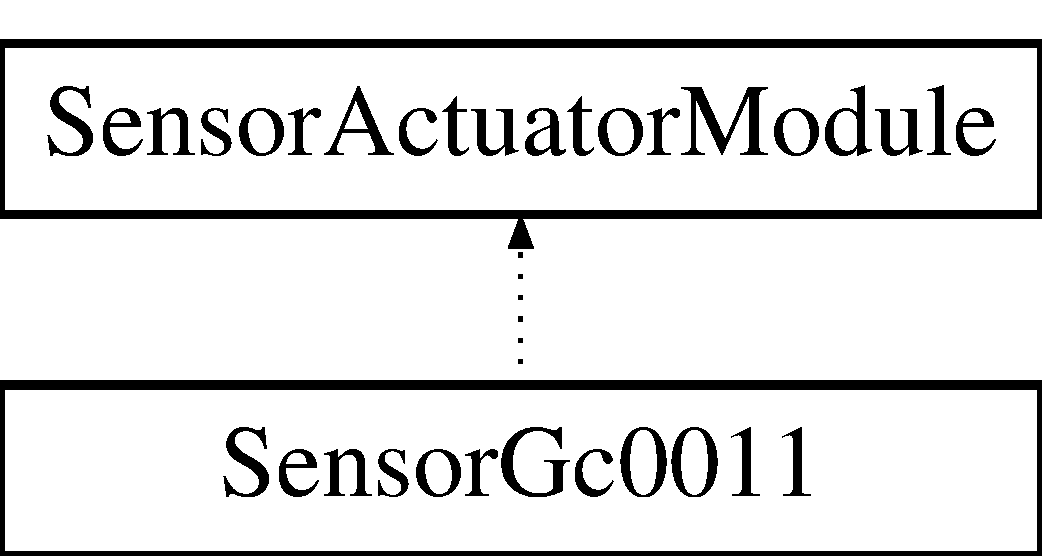
\includegraphics[height=2.000000cm]{class_sensor_gc0011}
\end{center}
\end{figure}
\subsection*{Public Member Functions}
\begin{DoxyCompactItemize}
\item 
\hyperlink{class_sensor_gc0011_ac8b12368b4b524198210048fbd1d0c81}{Sensor\+Gc0011} (int rx\+\_\+pin, int tx\+\_\+pin, String co2\+\_\+instruction\+\_\+code, int co2\+\_\+instruction\+\_\+id, String temperature\+\_\+instruction\+\_\+code, int temperature\+\_\+instruction\+\_\+id, String humidity\+\_\+instruction\+\_\+code, int humidity\+\_\+instruction\+\_\+id)
\item 
void \hyperlink{class_sensor_gc0011_a661743d47448c6b9c965fd8e1f123fbc}{begin} (void)
\begin{DoxyCompactList}\small\item\em Called once at beginning of program to initialize modules. \end{DoxyCompactList}\item 
String \hyperlink{class_sensor_gc0011_a2920401f54e121bba1398d52e9b2c90a}{get} (void)
\begin{DoxyCompactList}\small\item\em Called once per loop iteration to update and report module data to controller. \end{DoxyCompactList}\item 
String \hyperlink{class_sensor_gc0011_a658b7856221577342b54e4dc7fe06d2a}{set} (String instruction\+\_\+code, int instruction\+\_\+id, String instruction\+\_\+parameter)
\begin{DoxyCompactList}\small\item\em Called once per loop iteration to update module state. If response is generated from updating, reports response to controller. \end{DoxyCompactList}\end{DoxyCompactItemize}
\subsection*{Public Attributes}
\begin{DoxyCompactItemize}
\item 
float \hyperlink{class_sensor_gc0011_a6da77eb384ff77e28c2fa092a03a4cbb}{temperature}
\item 
float \hyperlink{class_sensor_gc0011_af5964ea62f030dd4ea2f219224afa4e6}{humidity}
\item 
float \hyperlink{class_sensor_gc0011_acd7c57373be1c5fb21c8da8c25861138}{co2}
\end{DoxyCompactItemize}


\subsection{Detailed Description}
Sensor module for air co2, temperature, and humidity. 

\subsection{Constructor \& Destructor Documentation}
\hypertarget{class_sensor_gc0011_ac8b12368b4b524198210048fbd1d0c81}{}\index{Sensor\+Gc0011@{Sensor\+Gc0011}!Sensor\+Gc0011@{Sensor\+Gc0011}}
\index{Sensor\+Gc0011@{Sensor\+Gc0011}!Sensor\+Gc0011@{Sensor\+Gc0011}}
\subsubsection[{Sensor\+Gc0011}]{\setlength{\rightskip}{0pt plus 5cm}Sensor\+Gc0011\+::\+Sensor\+Gc0011 (
\begin{DoxyParamCaption}
\item[{int}]{rx\+\_\+pin, }
\item[{int}]{tx\+\_\+pin, }
\item[{String}]{co2\+\_\+instruction\+\_\+code, }
\item[{int}]{co2\+\_\+instruction\+\_\+id, }
\item[{String}]{temperature\+\_\+instruction\+\_\+code, }
\item[{int}]{temperature\+\_\+instruction\+\_\+id, }
\item[{String}]{humidity\+\_\+instruction\+\_\+code, }
\item[{int}]{humidity\+\_\+instruction\+\_\+id}
\end{DoxyParamCaption}
)}\label{class_sensor_gc0011_ac8b12368b4b524198210048fbd1d0c81}


\subsection{Member Function Documentation}
\hypertarget{class_sensor_gc0011_a661743d47448c6b9c965fd8e1f123fbc}{}\index{Sensor\+Gc0011@{Sensor\+Gc0011}!begin@{begin}}
\index{begin@{begin}!Sensor\+Gc0011@{Sensor\+Gc0011}}
\subsubsection[{begin}]{\setlength{\rightskip}{0pt plus 5cm}void Sensor\+Gc0011\+::begin (
\begin{DoxyParamCaption}
\item[{void}]{}
\end{DoxyParamCaption}
)\hspace{0.3cm}{\ttfamily [virtual]}}\label{class_sensor_gc0011_a661743d47448c6b9c965fd8e1f123fbc}


Called once at beginning of program to initialize modules. 



Implements \hyperlink{class_sensor_actuator_module_a453094bcf7c7a2fdb2a14f65bf18bff9}{Sensor\+Actuator\+Module}.

\hypertarget{class_sensor_gc0011_a2920401f54e121bba1398d52e9b2c90a}{}\index{Sensor\+Gc0011@{Sensor\+Gc0011}!get@{get}}
\index{get@{get}!Sensor\+Gc0011@{Sensor\+Gc0011}}
\subsubsection[{get}]{\setlength{\rightskip}{0pt plus 5cm}String Sensor\+Gc0011\+::get (
\begin{DoxyParamCaption}
\item[{void}]{}
\end{DoxyParamCaption}
)\hspace{0.3cm}{\ttfamily [virtual]}}\label{class_sensor_gc0011_a2920401f54e121bba1398d52e9b2c90a}


Called once per loop iteration to update and report module data to controller. 



Implements \hyperlink{class_sensor_actuator_module_a55ce31fe50fc64f90602f3f70c5dc1af}{Sensor\+Actuator\+Module}.

\hypertarget{class_sensor_gc0011_a658b7856221577342b54e4dc7fe06d2a}{}\index{Sensor\+Gc0011@{Sensor\+Gc0011}!set@{set}}
\index{set@{set}!Sensor\+Gc0011@{Sensor\+Gc0011}}
\subsubsection[{set}]{\setlength{\rightskip}{0pt plus 5cm}String Sensor\+Gc0011\+::set (
\begin{DoxyParamCaption}
\item[{String}]{instruction\+\_\+code, }
\item[{int}]{instruction\+\_\+id, }
\item[{String}]{instruction\+\_\+parameter}
\end{DoxyParamCaption}
)\hspace{0.3cm}{\ttfamily [virtual]}}\label{class_sensor_gc0011_a658b7856221577342b54e4dc7fe06d2a}


Called once per loop iteration to update module state. If response is generated from updating, reports response to controller. 



Implements \hyperlink{class_sensor_actuator_module_adf93ff40fbdfeecbb8711ea0626fe6fc}{Sensor\+Actuator\+Module}.



\subsection{Member Data Documentation}
\hypertarget{class_sensor_gc0011_acd7c57373be1c5fb21c8da8c25861138}{}\index{Sensor\+Gc0011@{Sensor\+Gc0011}!co2@{co2}}
\index{co2@{co2}!Sensor\+Gc0011@{Sensor\+Gc0011}}
\subsubsection[{co2}]{\setlength{\rightskip}{0pt plus 5cm}float Sensor\+Gc0011\+::co2}\label{class_sensor_gc0011_acd7c57373be1c5fb21c8da8c25861138}
\hypertarget{class_sensor_gc0011_af5964ea62f030dd4ea2f219224afa4e6}{}\index{Sensor\+Gc0011@{Sensor\+Gc0011}!humidity@{humidity}}
\index{humidity@{humidity}!Sensor\+Gc0011@{Sensor\+Gc0011}}
\subsubsection[{humidity}]{\setlength{\rightskip}{0pt plus 5cm}float Sensor\+Gc0011\+::humidity}\label{class_sensor_gc0011_af5964ea62f030dd4ea2f219224afa4e6}
\hypertarget{class_sensor_gc0011_a6da77eb384ff77e28c2fa092a03a4cbb}{}\index{Sensor\+Gc0011@{Sensor\+Gc0011}!temperature@{temperature}}
\index{temperature@{temperature}!Sensor\+Gc0011@{Sensor\+Gc0011}}
\subsubsection[{temperature}]{\setlength{\rightskip}{0pt plus 5cm}float Sensor\+Gc0011\+::temperature}\label{class_sensor_gc0011_a6da77eb384ff77e28c2fa092a03a4cbb}


The documentation for this class was generated from the following files\+:\begin{DoxyCompactItemize}
\item 
src/\hyperlink{sensor__gc0011_8h}{sensor\+\_\+gc0011.\+h}\item 
src/\hyperlink{sensor__gc0011_8cpp}{sensor\+\_\+gc0011.\+cpp}\end{DoxyCompactItemize}

\hypertarget{class_sensor_tsl2561}{}\section{Sensor\+Tsl2561 Class Reference}
\label{class_sensor_tsl2561}\index{Sensor\+Tsl2561@{Sensor\+Tsl2561}}


Sensor module for light intensity and par.  




{\ttfamily \#include $<$sensor\+\_\+tsl2561.\+h$>$}

Inheritance diagram for Sensor\+Tsl2561\+:\begin{figure}[H]
\begin{center}
\leavevmode
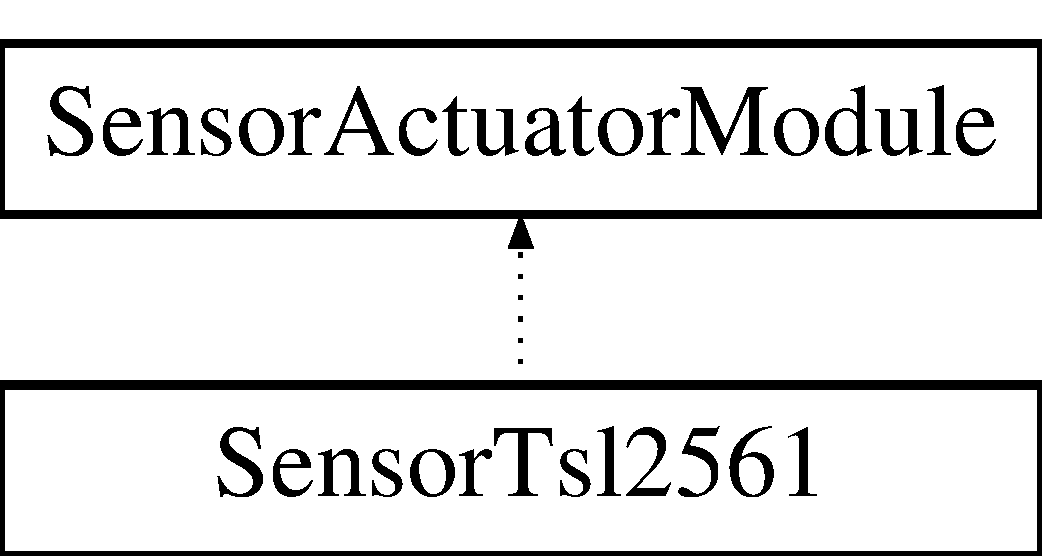
\includegraphics[height=2.000000cm]{class_sensor_tsl2561}
\end{center}
\end{figure}
\subsection*{Public Member Functions}
\begin{DoxyCompactItemize}
\item 
\hyperlink{class_sensor_tsl2561_acb66b0b6127d1d889ff31085dbb9d8c2}{Sensor\+Tsl2561} (String lux\+\_\+instruction\+\_\+code, int lux\+\_\+instruction\+\_\+id, String par\+\_\+instruction\+\_\+code, int par\+\_\+instruction\+\_\+id)
\item 
void \hyperlink{class_sensor_tsl2561_ace17c892222366185df021bda708cc10}{begin} (void)
\begin{DoxyCompactList}\small\item\em Called once at beginning of program to initialize modules. \end{DoxyCompactList}\item 
String \hyperlink{class_sensor_tsl2561_a1d9dff52af755218abca50f9025f0f5c}{get} (void)
\begin{DoxyCompactList}\small\item\em Called once per loop iteration to update and report module data to controller. \end{DoxyCompactList}\item 
String \hyperlink{class_sensor_tsl2561_ab4eb3d8197c96867f43857876df46b33}{set} (String instruction\+\_\+code, int instruction\+\_\+id, String instruction\+\_\+parameter)
\begin{DoxyCompactList}\small\item\em Called once per loop iteration to update module state. If response is generated from updating, reports response to controller. \end{DoxyCompactList}\end{DoxyCompactItemize}
\subsection*{Public Attributes}
\begin{DoxyCompactItemize}
\item 
int \hyperlink{class_sensor_tsl2561_ae12c0a6210834b63eb786e81043c38c4}{lux\+\_\+}
\item 
float \hyperlink{class_sensor_tsl2561_a1159f0229bf7cfc07da35366f81661f7}{par\+\_\+}
\end{DoxyCompactItemize}


\subsection{Detailed Description}
Sensor module for light intensity and par. 

\subsection{Constructor \& Destructor Documentation}
\hypertarget{class_sensor_tsl2561_acb66b0b6127d1d889ff31085dbb9d8c2}{}\index{Sensor\+Tsl2561@{Sensor\+Tsl2561}!Sensor\+Tsl2561@{Sensor\+Tsl2561}}
\index{Sensor\+Tsl2561@{Sensor\+Tsl2561}!Sensor\+Tsl2561@{Sensor\+Tsl2561}}
\subsubsection[{Sensor\+Tsl2561}]{\setlength{\rightskip}{0pt plus 5cm}Sensor\+Tsl2561\+::\+Sensor\+Tsl2561 (
\begin{DoxyParamCaption}
\item[{String}]{lux\+\_\+instruction\+\_\+code, }
\item[{int}]{lux\+\_\+instruction\+\_\+id, }
\item[{String}]{par\+\_\+instruction\+\_\+code, }
\item[{int}]{par\+\_\+instruction\+\_\+id}
\end{DoxyParamCaption}
)}\label{class_sensor_tsl2561_acb66b0b6127d1d889ff31085dbb9d8c2}


\subsection{Member Function Documentation}
\hypertarget{class_sensor_tsl2561_ace17c892222366185df021bda708cc10}{}\index{Sensor\+Tsl2561@{Sensor\+Tsl2561}!begin@{begin}}
\index{begin@{begin}!Sensor\+Tsl2561@{Sensor\+Tsl2561}}
\subsubsection[{begin}]{\setlength{\rightskip}{0pt plus 5cm}void Sensor\+Tsl2561\+::begin (
\begin{DoxyParamCaption}
\item[{void}]{}
\end{DoxyParamCaption}
)\hspace{0.3cm}{\ttfamily [virtual]}}\label{class_sensor_tsl2561_ace17c892222366185df021bda708cc10}


Called once at beginning of program to initialize modules. 



Implements \hyperlink{class_sensor_actuator_module_a453094bcf7c7a2fdb2a14f65bf18bff9}{Sensor\+Actuator\+Module}.

\hypertarget{class_sensor_tsl2561_a1d9dff52af755218abca50f9025f0f5c}{}\index{Sensor\+Tsl2561@{Sensor\+Tsl2561}!get@{get}}
\index{get@{get}!Sensor\+Tsl2561@{Sensor\+Tsl2561}}
\subsubsection[{get}]{\setlength{\rightskip}{0pt plus 5cm}String Sensor\+Tsl2561\+::get (
\begin{DoxyParamCaption}
\item[{void}]{}
\end{DoxyParamCaption}
)\hspace{0.3cm}{\ttfamily [virtual]}}\label{class_sensor_tsl2561_a1d9dff52af755218abca50f9025f0f5c}


Called once per loop iteration to update and report module data to controller. 



Implements \hyperlink{class_sensor_actuator_module_a55ce31fe50fc64f90602f3f70c5dc1af}{Sensor\+Actuator\+Module}.

\hypertarget{class_sensor_tsl2561_ab4eb3d8197c96867f43857876df46b33}{}\index{Sensor\+Tsl2561@{Sensor\+Tsl2561}!set@{set}}
\index{set@{set}!Sensor\+Tsl2561@{Sensor\+Tsl2561}}
\subsubsection[{set}]{\setlength{\rightskip}{0pt plus 5cm}String Sensor\+Tsl2561\+::set (
\begin{DoxyParamCaption}
\item[{String}]{instruction\+\_\+code, }
\item[{int}]{instruction\+\_\+id, }
\item[{String}]{instruction\+\_\+parameter}
\end{DoxyParamCaption}
)\hspace{0.3cm}{\ttfamily [virtual]}}\label{class_sensor_tsl2561_ab4eb3d8197c96867f43857876df46b33}


Called once per loop iteration to update module state. If response is generated from updating, reports response to controller. 



Implements \hyperlink{class_sensor_actuator_module_adf93ff40fbdfeecbb8711ea0626fe6fc}{Sensor\+Actuator\+Module}.



\subsection{Member Data Documentation}
\hypertarget{class_sensor_tsl2561_ae12c0a6210834b63eb786e81043c38c4}{}\index{Sensor\+Tsl2561@{Sensor\+Tsl2561}!lux\+\_\+@{lux\+\_\+}}
\index{lux\+\_\+@{lux\+\_\+}!Sensor\+Tsl2561@{Sensor\+Tsl2561}}
\subsubsection[{lux\+\_\+}]{\setlength{\rightskip}{0pt plus 5cm}int Sensor\+Tsl2561\+::lux\+\_\+}\label{class_sensor_tsl2561_ae12c0a6210834b63eb786e81043c38c4}
\hypertarget{class_sensor_tsl2561_a1159f0229bf7cfc07da35366f81661f7}{}\index{Sensor\+Tsl2561@{Sensor\+Tsl2561}!par\+\_\+@{par\+\_\+}}
\index{par\+\_\+@{par\+\_\+}!Sensor\+Tsl2561@{Sensor\+Tsl2561}}
\subsubsection[{par\+\_\+}]{\setlength{\rightskip}{0pt plus 5cm}float Sensor\+Tsl2561\+::par\+\_\+}\label{class_sensor_tsl2561_a1159f0229bf7cfc07da35366f81661f7}


The documentation for this class was generated from the following files\+:\begin{DoxyCompactItemize}
\item 
src/\hyperlink{sensor__tsl2561_8h}{sensor\+\_\+tsl2561.\+h}\item 
src/\hyperlink{sensor__tsl2561_8cpp}{sensor\+\_\+tsl2561.\+cpp}\end{DoxyCompactItemize}

\hypertarget{class_software_serial}{}\section{Software\+Serial Class Reference}
\label{class_software_serial}\index{Software\+Serial@{Software\+Serial}}


{\ttfamily \#include $<$support\+\_\+software\+\_\+serial.\+h$>$}

Inheritance diagram for Software\+Serial\+:\begin{figure}[H]
\begin{center}
\leavevmode
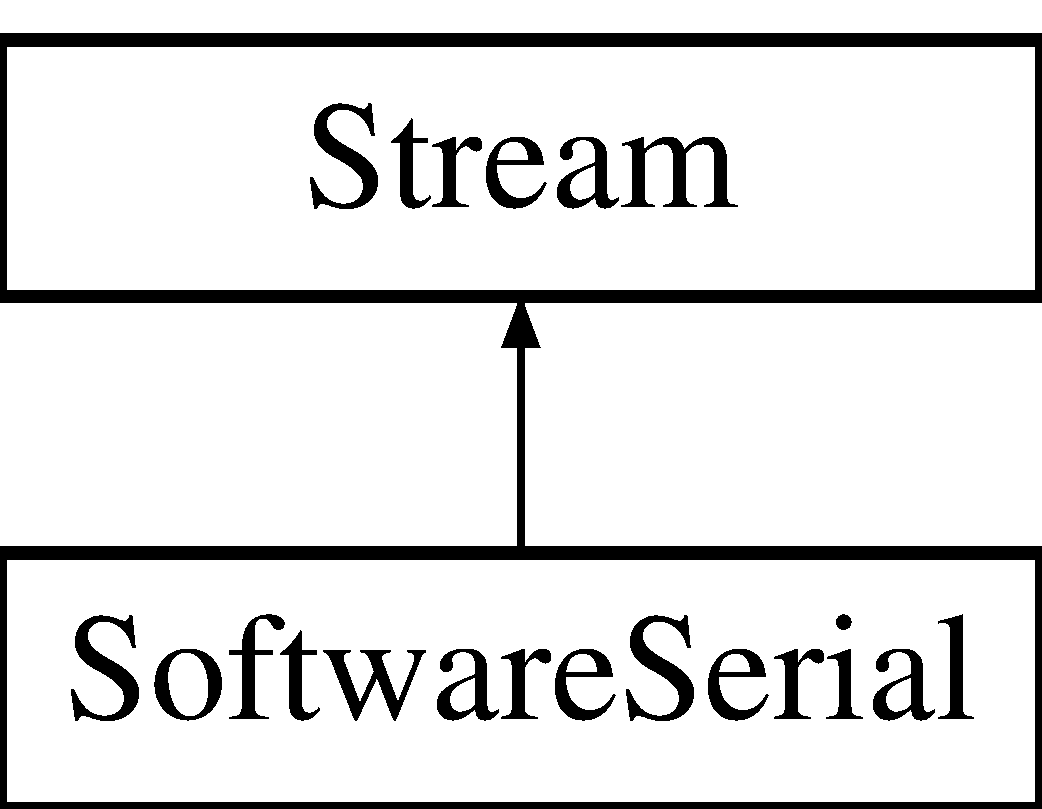
\includegraphics[height=2.000000cm]{class_software_serial}
\end{center}
\end{figure}
\subsection*{Public Member Functions}
\begin{DoxyCompactItemize}
\item 
\hyperlink{class_software_serial_aab36336db4a1ca5073071c07d910cb87}{Software\+Serial} (uint8\+\_\+t receive\+Pin, uint8\+\_\+t transmit\+Pin, bool inverse\+\_\+logic=false)
\item 
\hyperlink{class_software_serial_af6b8fff282e09a6cecc5df669ae71ee7}{$\sim$\+Software\+Serial} ()
\item 
void \hyperlink{class_software_serial_af1b194359d70894b3a2f38236a68480e}{begin} (long speed)
\item 
bool \hyperlink{class_software_serial_ad235539ef28939836bd0bde9387eb8fc}{listen} ()
\item 
void \hyperlink{class_software_serial_a9034270f7de617b3cc7d3f38f3a8e0df}{end} ()
\item 
bool \hyperlink{class_software_serial_a7b3fb4a8f57d2b5f2233f841d71ef80f}{is\+Listening} ()
\item 
bool \hyperlink{class_software_serial_a1c87a6b43c176c104f28e2c2eec2841e}{stop\+Listening} ()
\item 
bool \hyperlink{class_software_serial_ac6d4d5dfbe05515bf23766e2c8abfd46}{overflow} ()
\item 
int \hyperlink{class_software_serial_a51c2d2e79f0d982b1ef9cc9ac4453648}{peek} ()
\item 
virtual size\+\_\+t \hyperlink{class_software_serial_ac24e5c6af203ec636c0a200b0cb3caf0}{write} (uint8\+\_\+t byte)
\item 
virtual int \hyperlink{class_software_serial_a2d0b2f2868d519c716114777f482705b}{read} ()
\item 
virtual int \hyperlink{class_software_serial_a4cbf77a4e90e15ca576972d7952659c5}{available} ()
\item 
virtual void \hyperlink{class_software_serial_a9a46db376a19fc958e011e38799b902c}{flush} ()
\item 
\hyperlink{class_software_serial_ab0cba63b2a27fcfa4760a2f3f7389de0}{operator bool} ()
\end{DoxyCompactItemize}
\subsection*{Static Public Member Functions}
\begin{DoxyCompactItemize}
\item 
static void \hyperlink{class_software_serial_a8700c768d3c5d681362253324852ceee}{handle\+\_\+interrupt} () \+\_\+\+\_\+attribute\+\_\+\+\_\+((\+\_\+\+\_\+always\+\_\+inline\+\_\+\+\_\+))
\end{DoxyCompactItemize}


\subsection{Constructor \& Destructor Documentation}
\hypertarget{class_software_serial_aab36336db4a1ca5073071c07d910cb87}{}\index{Software\+Serial@{Software\+Serial}!Software\+Serial@{Software\+Serial}}
\index{Software\+Serial@{Software\+Serial}!Software\+Serial@{Software\+Serial}}
\subsubsection[{Software\+Serial}]{\setlength{\rightskip}{0pt plus 5cm}Software\+Serial\+::\+Software\+Serial (
\begin{DoxyParamCaption}
\item[{uint8\+\_\+t}]{receive\+Pin, }
\item[{uint8\+\_\+t}]{transmit\+Pin, }
\item[{bool}]{inverse\+\_\+logic = {\ttfamily false}}
\end{DoxyParamCaption}
)}\label{class_software_serial_aab36336db4a1ca5073071c07d910cb87}
\hypertarget{class_software_serial_af6b8fff282e09a6cecc5df669ae71ee7}{}\index{Software\+Serial@{Software\+Serial}!````~Software\+Serial@{$\sim$\+Software\+Serial}}
\index{````~Software\+Serial@{$\sim$\+Software\+Serial}!Software\+Serial@{Software\+Serial}}
\subsubsection[{$\sim$\+Software\+Serial}]{\setlength{\rightskip}{0pt plus 5cm}Software\+Serial\+::$\sim$\+Software\+Serial (
\begin{DoxyParamCaption}
{}
\end{DoxyParamCaption}
)}\label{class_software_serial_af6b8fff282e09a6cecc5df669ae71ee7}


\subsection{Member Function Documentation}
\hypertarget{class_software_serial_a4cbf77a4e90e15ca576972d7952659c5}{}\index{Software\+Serial@{Software\+Serial}!available@{available}}
\index{available@{available}!Software\+Serial@{Software\+Serial}}
\subsubsection[{available}]{\setlength{\rightskip}{0pt plus 5cm}int Software\+Serial\+::available (
\begin{DoxyParamCaption}
\item[{void}]{}
\end{DoxyParamCaption}
)\hspace{0.3cm}{\ttfamily [virtual]}}\label{class_software_serial_a4cbf77a4e90e15ca576972d7952659c5}
\hypertarget{class_software_serial_af1b194359d70894b3a2f38236a68480e}{}\index{Software\+Serial@{Software\+Serial}!begin@{begin}}
\index{begin@{begin}!Software\+Serial@{Software\+Serial}}
\subsubsection[{begin}]{\setlength{\rightskip}{0pt plus 5cm}void Software\+Serial\+::begin (
\begin{DoxyParamCaption}
\item[{long}]{speed}
\end{DoxyParamCaption}
)}\label{class_software_serial_af1b194359d70894b3a2f38236a68480e}
\hypertarget{class_software_serial_a9034270f7de617b3cc7d3f38f3a8e0df}{}\index{Software\+Serial@{Software\+Serial}!end@{end}}
\index{end@{end}!Software\+Serial@{Software\+Serial}}
\subsubsection[{end}]{\setlength{\rightskip}{0pt plus 5cm}void Software\+Serial\+::end (
\begin{DoxyParamCaption}
{}
\end{DoxyParamCaption}
)}\label{class_software_serial_a9034270f7de617b3cc7d3f38f3a8e0df}
\hypertarget{class_software_serial_a9a46db376a19fc958e011e38799b902c}{}\index{Software\+Serial@{Software\+Serial}!flush@{flush}}
\index{flush@{flush}!Software\+Serial@{Software\+Serial}}
\subsubsection[{flush}]{\setlength{\rightskip}{0pt plus 5cm}void Software\+Serial\+::flush (
\begin{DoxyParamCaption}
{}
\end{DoxyParamCaption}
)\hspace{0.3cm}{\ttfamily [virtual]}}\label{class_software_serial_a9a46db376a19fc958e011e38799b902c}
\hypertarget{class_software_serial_a8700c768d3c5d681362253324852ceee}{}\index{Software\+Serial@{Software\+Serial}!handle\+\_\+interrupt@{handle\+\_\+interrupt}}
\index{handle\+\_\+interrupt@{handle\+\_\+interrupt}!Software\+Serial@{Software\+Serial}}
\subsubsection[{handle\+\_\+interrupt}]{\setlength{\rightskip}{0pt plus 5cm}void Software\+Serial\+::handle\+\_\+interrupt (
\begin{DoxyParamCaption}
{}
\end{DoxyParamCaption}
)\hspace{0.3cm}{\ttfamily [inline]}, {\ttfamily [static]}}\label{class_software_serial_a8700c768d3c5d681362253324852ceee}
\hypertarget{class_software_serial_a7b3fb4a8f57d2b5f2233f841d71ef80f}{}\index{Software\+Serial@{Software\+Serial}!is\+Listening@{is\+Listening}}
\index{is\+Listening@{is\+Listening}!Software\+Serial@{Software\+Serial}}
\subsubsection[{is\+Listening}]{\setlength{\rightskip}{0pt plus 5cm}bool Software\+Serial\+::is\+Listening (
\begin{DoxyParamCaption}
{}
\end{DoxyParamCaption}
)\hspace{0.3cm}{\ttfamily [inline]}}\label{class_software_serial_a7b3fb4a8f57d2b5f2233f841d71ef80f}
\hypertarget{class_software_serial_ad235539ef28939836bd0bde9387eb8fc}{}\index{Software\+Serial@{Software\+Serial}!listen@{listen}}
\index{listen@{listen}!Software\+Serial@{Software\+Serial}}
\subsubsection[{listen}]{\setlength{\rightskip}{0pt plus 5cm}bool Software\+Serial\+::listen (
\begin{DoxyParamCaption}
{}
\end{DoxyParamCaption}
)}\label{class_software_serial_ad235539ef28939836bd0bde9387eb8fc}
\hypertarget{class_software_serial_ab0cba63b2a27fcfa4760a2f3f7389de0}{}\index{Software\+Serial@{Software\+Serial}!operator bool@{operator bool}}
\index{operator bool@{operator bool}!Software\+Serial@{Software\+Serial}}
\subsubsection[{operator bool}]{\setlength{\rightskip}{0pt plus 5cm}Software\+Serial\+::operator bool (
\begin{DoxyParamCaption}
{}
\end{DoxyParamCaption}
)\hspace{0.3cm}{\ttfamily [inline]}}\label{class_software_serial_ab0cba63b2a27fcfa4760a2f3f7389de0}
\hypertarget{class_software_serial_ac6d4d5dfbe05515bf23766e2c8abfd46}{}\index{Software\+Serial@{Software\+Serial}!overflow@{overflow}}
\index{overflow@{overflow}!Software\+Serial@{Software\+Serial}}
\subsubsection[{overflow}]{\setlength{\rightskip}{0pt plus 5cm}bool Software\+Serial\+::overflow (
\begin{DoxyParamCaption}
{}
\end{DoxyParamCaption}
)\hspace{0.3cm}{\ttfamily [inline]}}\label{class_software_serial_ac6d4d5dfbe05515bf23766e2c8abfd46}
\hypertarget{class_software_serial_a51c2d2e79f0d982b1ef9cc9ac4453648}{}\index{Software\+Serial@{Software\+Serial}!peek@{peek}}
\index{peek@{peek}!Software\+Serial@{Software\+Serial}}
\subsubsection[{peek}]{\setlength{\rightskip}{0pt plus 5cm}int Software\+Serial\+::peek (
\begin{DoxyParamCaption}
{}
\end{DoxyParamCaption}
)}\label{class_software_serial_a51c2d2e79f0d982b1ef9cc9ac4453648}
\hypertarget{class_software_serial_a2d0b2f2868d519c716114777f482705b}{}\index{Software\+Serial@{Software\+Serial}!read@{read}}
\index{read@{read}!Software\+Serial@{Software\+Serial}}
\subsubsection[{read}]{\setlength{\rightskip}{0pt plus 5cm}int Software\+Serial\+::read (
\begin{DoxyParamCaption}
\item[{void}]{}
\end{DoxyParamCaption}
)\hspace{0.3cm}{\ttfamily [virtual]}}\label{class_software_serial_a2d0b2f2868d519c716114777f482705b}
\hypertarget{class_software_serial_a1c87a6b43c176c104f28e2c2eec2841e}{}\index{Software\+Serial@{Software\+Serial}!stop\+Listening@{stop\+Listening}}
\index{stop\+Listening@{stop\+Listening}!Software\+Serial@{Software\+Serial}}
\subsubsection[{stop\+Listening}]{\setlength{\rightskip}{0pt plus 5cm}bool Software\+Serial\+::stop\+Listening (
\begin{DoxyParamCaption}
{}
\end{DoxyParamCaption}
)}\label{class_software_serial_a1c87a6b43c176c104f28e2c2eec2841e}
\hypertarget{class_software_serial_ac24e5c6af203ec636c0a200b0cb3caf0}{}\index{Software\+Serial@{Software\+Serial}!write@{write}}
\index{write@{write}!Software\+Serial@{Software\+Serial}}
\subsubsection[{write}]{\setlength{\rightskip}{0pt plus 5cm}size\+\_\+t Software\+Serial\+::write (
\begin{DoxyParamCaption}
\item[{uint8\+\_\+t}]{byte}
\end{DoxyParamCaption}
)\hspace{0.3cm}{\ttfamily [virtual]}}\label{class_software_serial_ac24e5c6af203ec636c0a200b0cb3caf0}


The documentation for this class was generated from the following files\+:\begin{DoxyCompactItemize}
\item 
src/\hyperlink{support__software__serial_8h}{support\+\_\+software\+\_\+serial.\+h}\item 
src/\hyperlink{support__software__serial_8cpp}{support\+\_\+software\+\_\+serial.\+cpp}\end{DoxyCompactItemize}

\hypertarget{class_two_wire}{}\section{Two\+Wire Class Reference}
\label{class_two_wire}\index{Two\+Wire@{Two\+Wire}}


{\ttfamily \#include $<$support\+\_\+wire.\+h$>$}

Inheritance diagram for Two\+Wire\+:\begin{figure}[H]
\begin{center}
\leavevmode
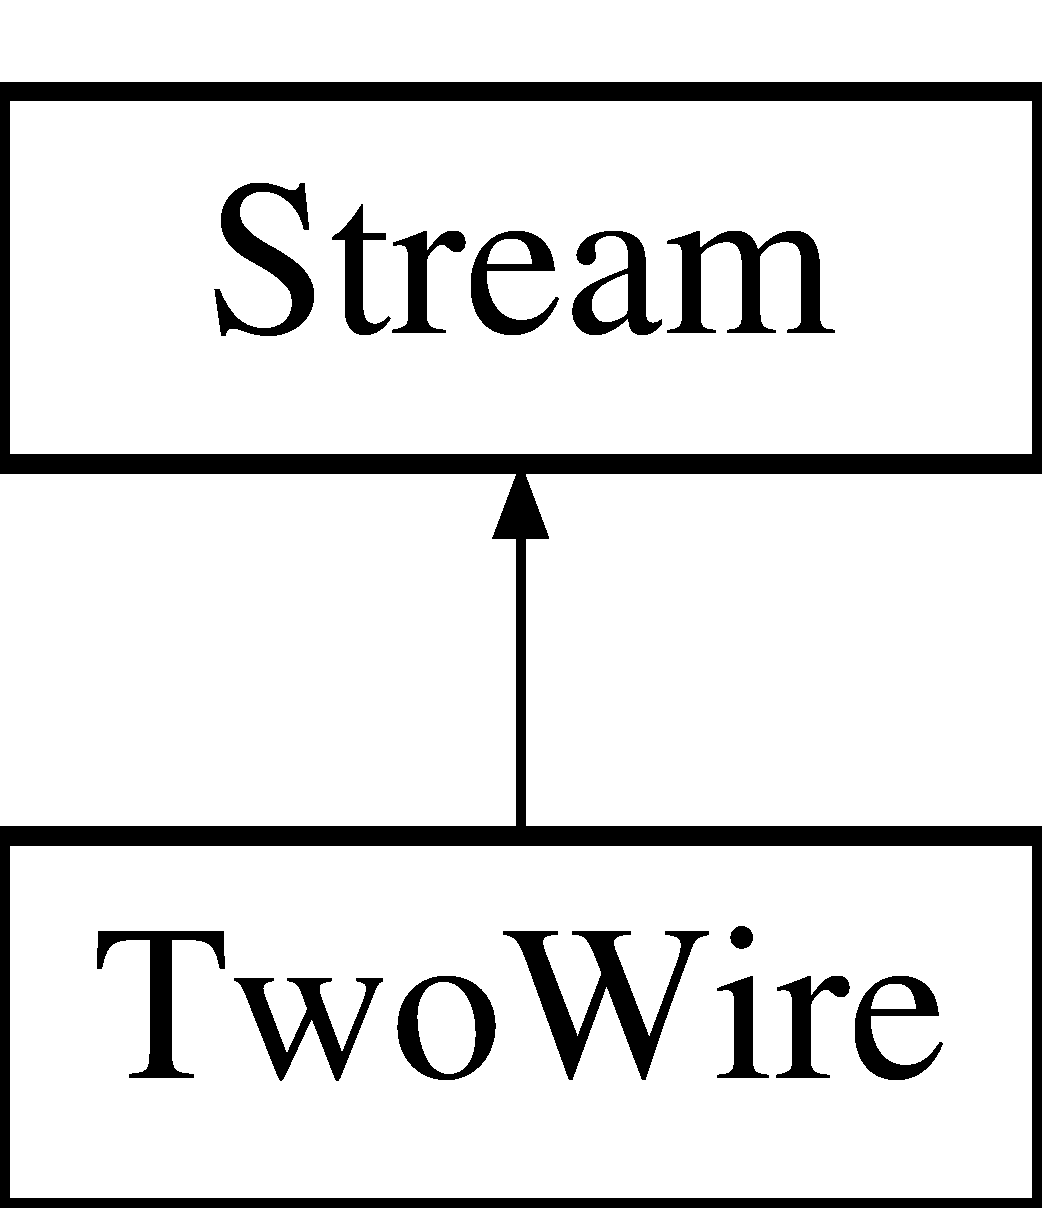
\includegraphics[height=2.000000cm]{class_two_wire}
\end{center}
\end{figure}
\subsection*{Public Member Functions}
\begin{DoxyCompactItemize}
\item 
\hyperlink{class_two_wire_a4c7daf378c06e5e72762e1bd3d5937b6}{Two\+Wire} ()
\item 
void \hyperlink{class_two_wire_ada85a7a8663ec8af0a1248b659be2f18}{begin} ()
\item 
void \hyperlink{class_two_wire_a28bca087ed188781ef15e72622d3b1fb}{begin} (uint8\+\_\+t)
\item 
void \hyperlink{class_two_wire_a2806aa5684d36d7d20bf7c51cab3e602}{begin} (int)
\item 
void \hyperlink{class_two_wire_a3c4aaae8779a8c34d8a1a90ff317d982}{set\+Clock} (uint32\+\_\+t)
\item 
void \hyperlink{class_two_wire_a8d55f00ea8ac3d7427d62e0c71e95ec2}{begin\+Transmission} (uint8\+\_\+t)
\item 
void \hyperlink{class_two_wire_a4da95eb4adced5dad152344243e57aad}{begin\+Transmission} (int)
\item 
uint8\+\_\+t \hyperlink{class_two_wire_af80f9a7b85a3a81a035ca94c95bcdc1d}{end\+Transmission} (void)
\item 
uint8\+\_\+t \hyperlink{class_two_wire_a289f5ef9bb0f79b31095fd72402ed54a}{end\+Transmission} (uint8\+\_\+t)
\item 
uint8\+\_\+t \hyperlink{class_two_wire_ae27d0936487551a05a1e9901bc456599}{request\+From} (uint8\+\_\+t, uint8\+\_\+t)
\item 
uint8\+\_\+t \hyperlink{class_two_wire_a4b4b618531a04d5488a52583a3dfb173}{request\+From} (uint8\+\_\+t, uint8\+\_\+t, uint8\+\_\+t)
\item 
uint8\+\_\+t \hyperlink{class_two_wire_ad40a27213d0bb32f7b819aa8962fccd3}{request\+From} (int, int)
\item 
uint8\+\_\+t \hyperlink{class_two_wire_a3d76da36fb8571e0b5e8310e9f86f6fe}{request\+From} (int, int, int)
\item 
virtual size\+\_\+t \hyperlink{class_two_wire_a318b7bec156c1f1075a818c0ad3427d7}{write} (uint8\+\_\+t)
\item 
virtual size\+\_\+t \hyperlink{class_two_wire_a1957b4d5a6a997bdde436e9e40d131a7}{write} (const uint8\+\_\+t $\ast$, size\+\_\+t)
\item 
virtual int \hyperlink{class_two_wire_aee57bc52bee06508e231c5fc6bc35ada}{available} (void)
\item 
virtual int \hyperlink{class_two_wire_aa361b83500d00dfb93bb25b6473b33e9}{read} (void)
\item 
virtual int \hyperlink{class_two_wire_a5bd64cb7bd609e9470a15d96a0991ec8}{peek} (void)
\item 
virtual void \hyperlink{class_two_wire_a4d92ddf6ca349c815de1de15fca06b5e}{flush} (void)
\item 
void \hyperlink{class_two_wire_a860d97eb825c6fdca388f2f0577cc34a}{on\+Receive} (void($\ast$)(int))
\item 
void \hyperlink{class_two_wire_a224bf8799dda398fc0db223801852ca5}{on\+Request} (void($\ast$)(void))
\item 
size\+\_\+t \hyperlink{class_two_wire_a0c9d09ead8fcddf2a84781fe77d3c975}{write} (unsigned long n)
\item 
size\+\_\+t \hyperlink{class_two_wire_a55a9894186458e43852f6fb7c59bb066}{write} (long n)
\item 
size\+\_\+t \hyperlink{class_two_wire_afdb917746ee37f72e7452b4782e9527b}{write} (unsigned int n)
\item 
size\+\_\+t \hyperlink{class_two_wire_a8ec34b0d2a75e8b2751eb9f4332bd7c3}{write} (int n)
\end{DoxyCompactItemize}


\subsection{Constructor \& Destructor Documentation}
\hypertarget{class_two_wire_a4c7daf378c06e5e72762e1bd3d5937b6}{}\index{Two\+Wire@{Two\+Wire}!Two\+Wire@{Two\+Wire}}
\index{Two\+Wire@{Two\+Wire}!Two\+Wire@{Two\+Wire}}
\subsubsection[{Two\+Wire}]{\setlength{\rightskip}{0pt plus 5cm}Two\+Wire\+::\+Two\+Wire (
\begin{DoxyParamCaption}
{}
\end{DoxyParamCaption}
)}\label{class_two_wire_a4c7daf378c06e5e72762e1bd3d5937b6}


\subsection{Member Function Documentation}
\hypertarget{class_two_wire_aee57bc52bee06508e231c5fc6bc35ada}{}\index{Two\+Wire@{Two\+Wire}!available@{available}}
\index{available@{available}!Two\+Wire@{Two\+Wire}}
\subsubsection[{available}]{\setlength{\rightskip}{0pt plus 5cm}int Two\+Wire\+::available (
\begin{DoxyParamCaption}
\item[{void}]{}
\end{DoxyParamCaption}
)\hspace{0.3cm}{\ttfamily [virtual]}}\label{class_two_wire_aee57bc52bee06508e231c5fc6bc35ada}
\hypertarget{class_two_wire_ada85a7a8663ec8af0a1248b659be2f18}{}\index{Two\+Wire@{Two\+Wire}!begin@{begin}}
\index{begin@{begin}!Two\+Wire@{Two\+Wire}}
\subsubsection[{begin}]{\setlength{\rightskip}{0pt plus 5cm}void Two\+Wire\+::begin (
\begin{DoxyParamCaption}
\item[{void}]{}
\end{DoxyParamCaption}
)}\label{class_two_wire_ada85a7a8663ec8af0a1248b659be2f18}
\hypertarget{class_two_wire_a28bca087ed188781ef15e72622d3b1fb}{}\index{Two\+Wire@{Two\+Wire}!begin@{begin}}
\index{begin@{begin}!Two\+Wire@{Two\+Wire}}
\subsubsection[{begin}]{\setlength{\rightskip}{0pt plus 5cm}void Two\+Wire\+::begin (
\begin{DoxyParamCaption}
\item[{uint8\+\_\+t}]{address}
\end{DoxyParamCaption}
)}\label{class_two_wire_a28bca087ed188781ef15e72622d3b1fb}
\hypertarget{class_two_wire_a2806aa5684d36d7d20bf7c51cab3e602}{}\index{Two\+Wire@{Two\+Wire}!begin@{begin}}
\index{begin@{begin}!Two\+Wire@{Two\+Wire}}
\subsubsection[{begin}]{\setlength{\rightskip}{0pt plus 5cm}void Two\+Wire\+::begin (
\begin{DoxyParamCaption}
\item[{int}]{address}
\end{DoxyParamCaption}
)}\label{class_two_wire_a2806aa5684d36d7d20bf7c51cab3e602}
\hypertarget{class_two_wire_a8d55f00ea8ac3d7427d62e0c71e95ec2}{}\index{Two\+Wire@{Two\+Wire}!begin\+Transmission@{begin\+Transmission}}
\index{begin\+Transmission@{begin\+Transmission}!Two\+Wire@{Two\+Wire}}
\subsubsection[{begin\+Transmission}]{\setlength{\rightskip}{0pt plus 5cm}void Two\+Wire\+::begin\+Transmission (
\begin{DoxyParamCaption}
\item[{uint8\+\_\+t}]{address}
\end{DoxyParamCaption}
)}\label{class_two_wire_a8d55f00ea8ac3d7427d62e0c71e95ec2}
\hypertarget{class_two_wire_a4da95eb4adced5dad152344243e57aad}{}\index{Two\+Wire@{Two\+Wire}!begin\+Transmission@{begin\+Transmission}}
\index{begin\+Transmission@{begin\+Transmission}!Two\+Wire@{Two\+Wire}}
\subsubsection[{begin\+Transmission}]{\setlength{\rightskip}{0pt plus 5cm}void Two\+Wire\+::begin\+Transmission (
\begin{DoxyParamCaption}
\item[{int}]{address}
\end{DoxyParamCaption}
)}\label{class_two_wire_a4da95eb4adced5dad152344243e57aad}
\hypertarget{class_two_wire_af80f9a7b85a3a81a035ca94c95bcdc1d}{}\index{Two\+Wire@{Two\+Wire}!end\+Transmission@{end\+Transmission}}
\index{end\+Transmission@{end\+Transmission}!Two\+Wire@{Two\+Wire}}
\subsubsection[{end\+Transmission}]{\setlength{\rightskip}{0pt plus 5cm}uint8\+\_\+t Two\+Wire\+::end\+Transmission (
\begin{DoxyParamCaption}
\item[{void}]{}
\end{DoxyParamCaption}
)}\label{class_two_wire_af80f9a7b85a3a81a035ca94c95bcdc1d}
\hypertarget{class_two_wire_a289f5ef9bb0f79b31095fd72402ed54a}{}\index{Two\+Wire@{Two\+Wire}!end\+Transmission@{end\+Transmission}}
\index{end\+Transmission@{end\+Transmission}!Two\+Wire@{Two\+Wire}}
\subsubsection[{end\+Transmission}]{\setlength{\rightskip}{0pt plus 5cm}uint8\+\_\+t Two\+Wire\+::end\+Transmission (
\begin{DoxyParamCaption}
\item[{uint8\+\_\+t}]{send\+Stop}
\end{DoxyParamCaption}
)}\label{class_two_wire_a289f5ef9bb0f79b31095fd72402ed54a}
\hypertarget{class_two_wire_a4d92ddf6ca349c815de1de15fca06b5e}{}\index{Two\+Wire@{Two\+Wire}!flush@{flush}}
\index{flush@{flush}!Two\+Wire@{Two\+Wire}}
\subsubsection[{flush}]{\setlength{\rightskip}{0pt plus 5cm}void Two\+Wire\+::flush (
\begin{DoxyParamCaption}
\item[{void}]{}
\end{DoxyParamCaption}
)\hspace{0.3cm}{\ttfamily [virtual]}}\label{class_two_wire_a4d92ddf6ca349c815de1de15fca06b5e}
\hypertarget{class_two_wire_a860d97eb825c6fdca388f2f0577cc34a}{}\index{Two\+Wire@{Two\+Wire}!on\+Receive@{on\+Receive}}
\index{on\+Receive@{on\+Receive}!Two\+Wire@{Two\+Wire}}
\subsubsection[{on\+Receive}]{\setlength{\rightskip}{0pt plus 5cm}void Two\+Wire\+::on\+Receive (
\begin{DoxyParamCaption}
\item[{void($\ast$)(int)}]{function}
\end{DoxyParamCaption}
)}\label{class_two_wire_a860d97eb825c6fdca388f2f0577cc34a}
\hypertarget{class_two_wire_a224bf8799dda398fc0db223801852ca5}{}\index{Two\+Wire@{Two\+Wire}!on\+Request@{on\+Request}}
\index{on\+Request@{on\+Request}!Two\+Wire@{Two\+Wire}}
\subsubsection[{on\+Request}]{\setlength{\rightskip}{0pt plus 5cm}void Two\+Wire\+::on\+Request (
\begin{DoxyParamCaption}
\item[{void($\ast$)(void)}]{function}
\end{DoxyParamCaption}
)}\label{class_two_wire_a224bf8799dda398fc0db223801852ca5}
\hypertarget{class_two_wire_a5bd64cb7bd609e9470a15d96a0991ec8}{}\index{Two\+Wire@{Two\+Wire}!peek@{peek}}
\index{peek@{peek}!Two\+Wire@{Two\+Wire}}
\subsubsection[{peek}]{\setlength{\rightskip}{0pt plus 5cm}int Two\+Wire\+::peek (
\begin{DoxyParamCaption}
\item[{void}]{}
\end{DoxyParamCaption}
)\hspace{0.3cm}{\ttfamily [virtual]}}\label{class_two_wire_a5bd64cb7bd609e9470a15d96a0991ec8}
\hypertarget{class_two_wire_aa361b83500d00dfb93bb25b6473b33e9}{}\index{Two\+Wire@{Two\+Wire}!read@{read}}
\index{read@{read}!Two\+Wire@{Two\+Wire}}
\subsubsection[{read}]{\setlength{\rightskip}{0pt plus 5cm}int Two\+Wire\+::read (
\begin{DoxyParamCaption}
\item[{void}]{}
\end{DoxyParamCaption}
)\hspace{0.3cm}{\ttfamily [virtual]}}\label{class_two_wire_aa361b83500d00dfb93bb25b6473b33e9}
\hypertarget{class_two_wire_ae27d0936487551a05a1e9901bc456599}{}\index{Two\+Wire@{Two\+Wire}!request\+From@{request\+From}}
\index{request\+From@{request\+From}!Two\+Wire@{Two\+Wire}}
\subsubsection[{request\+From}]{\setlength{\rightskip}{0pt plus 5cm}uint8\+\_\+t Two\+Wire\+::request\+From (
\begin{DoxyParamCaption}
\item[{uint8\+\_\+t}]{address, }
\item[{uint8\+\_\+t}]{quantity}
\end{DoxyParamCaption}
)}\label{class_two_wire_ae27d0936487551a05a1e9901bc456599}
\hypertarget{class_two_wire_a4b4b618531a04d5488a52583a3dfb173}{}\index{Two\+Wire@{Two\+Wire}!request\+From@{request\+From}}
\index{request\+From@{request\+From}!Two\+Wire@{Two\+Wire}}
\subsubsection[{request\+From}]{\setlength{\rightskip}{0pt plus 5cm}uint8\+\_\+t Two\+Wire\+::request\+From (
\begin{DoxyParamCaption}
\item[{uint8\+\_\+t}]{address, }
\item[{uint8\+\_\+t}]{quantity, }
\item[{uint8\+\_\+t}]{send\+Stop}
\end{DoxyParamCaption}
)}\label{class_two_wire_a4b4b618531a04d5488a52583a3dfb173}
\hypertarget{class_two_wire_ad40a27213d0bb32f7b819aa8962fccd3}{}\index{Two\+Wire@{Two\+Wire}!request\+From@{request\+From}}
\index{request\+From@{request\+From}!Two\+Wire@{Two\+Wire}}
\subsubsection[{request\+From}]{\setlength{\rightskip}{0pt plus 5cm}uint8\+\_\+t Two\+Wire\+::request\+From (
\begin{DoxyParamCaption}
\item[{int}]{address, }
\item[{int}]{quantity}
\end{DoxyParamCaption}
)}\label{class_two_wire_ad40a27213d0bb32f7b819aa8962fccd3}
\hypertarget{class_two_wire_a3d76da36fb8571e0b5e8310e9f86f6fe}{}\index{Two\+Wire@{Two\+Wire}!request\+From@{request\+From}}
\index{request\+From@{request\+From}!Two\+Wire@{Two\+Wire}}
\subsubsection[{request\+From}]{\setlength{\rightskip}{0pt plus 5cm}uint8\+\_\+t Two\+Wire\+::request\+From (
\begin{DoxyParamCaption}
\item[{int}]{address, }
\item[{int}]{quantity, }
\item[{int}]{send\+Stop}
\end{DoxyParamCaption}
)}\label{class_two_wire_a3d76da36fb8571e0b5e8310e9f86f6fe}
\hypertarget{class_two_wire_a3c4aaae8779a8c34d8a1a90ff317d982}{}\index{Two\+Wire@{Two\+Wire}!set\+Clock@{set\+Clock}}
\index{set\+Clock@{set\+Clock}!Two\+Wire@{Two\+Wire}}
\subsubsection[{set\+Clock}]{\setlength{\rightskip}{0pt plus 5cm}void Two\+Wire\+::set\+Clock (
\begin{DoxyParamCaption}
\item[{uint32\+\_\+t}]{frequency}
\end{DoxyParamCaption}
)}\label{class_two_wire_a3c4aaae8779a8c34d8a1a90ff317d982}
\hypertarget{class_two_wire_a318b7bec156c1f1075a818c0ad3427d7}{}\index{Two\+Wire@{Two\+Wire}!write@{write}}
\index{write@{write}!Two\+Wire@{Two\+Wire}}
\subsubsection[{write}]{\setlength{\rightskip}{0pt plus 5cm}size\+\_\+t Two\+Wire\+::write (
\begin{DoxyParamCaption}
\item[{uint8\+\_\+t}]{data}
\end{DoxyParamCaption}
)\hspace{0.3cm}{\ttfamily [virtual]}}\label{class_two_wire_a318b7bec156c1f1075a818c0ad3427d7}
\hypertarget{class_two_wire_a1957b4d5a6a997bdde436e9e40d131a7}{}\index{Two\+Wire@{Two\+Wire}!write@{write}}
\index{write@{write}!Two\+Wire@{Two\+Wire}}
\subsubsection[{write}]{\setlength{\rightskip}{0pt plus 5cm}size\+\_\+t Two\+Wire\+::write (
\begin{DoxyParamCaption}
\item[{const uint8\+\_\+t $\ast$}]{data, }
\item[{size\+\_\+t}]{quantity}
\end{DoxyParamCaption}
)\hspace{0.3cm}{\ttfamily [virtual]}}\label{class_two_wire_a1957b4d5a6a997bdde436e9e40d131a7}
\hypertarget{class_two_wire_a0c9d09ead8fcddf2a84781fe77d3c975}{}\index{Two\+Wire@{Two\+Wire}!write@{write}}
\index{write@{write}!Two\+Wire@{Two\+Wire}}
\subsubsection[{write}]{\setlength{\rightskip}{0pt plus 5cm}size\+\_\+t Two\+Wire\+::write (
\begin{DoxyParamCaption}
\item[{unsigned long}]{n}
\end{DoxyParamCaption}
)\hspace{0.3cm}{\ttfamily [inline]}}\label{class_two_wire_a0c9d09ead8fcddf2a84781fe77d3c975}
\hypertarget{class_two_wire_a55a9894186458e43852f6fb7c59bb066}{}\index{Two\+Wire@{Two\+Wire}!write@{write}}
\index{write@{write}!Two\+Wire@{Two\+Wire}}
\subsubsection[{write}]{\setlength{\rightskip}{0pt plus 5cm}size\+\_\+t Two\+Wire\+::write (
\begin{DoxyParamCaption}
\item[{long}]{n}
\end{DoxyParamCaption}
)\hspace{0.3cm}{\ttfamily [inline]}}\label{class_two_wire_a55a9894186458e43852f6fb7c59bb066}
\hypertarget{class_two_wire_afdb917746ee37f72e7452b4782e9527b}{}\index{Two\+Wire@{Two\+Wire}!write@{write}}
\index{write@{write}!Two\+Wire@{Two\+Wire}}
\subsubsection[{write}]{\setlength{\rightskip}{0pt plus 5cm}size\+\_\+t Two\+Wire\+::write (
\begin{DoxyParamCaption}
\item[{unsigned int}]{n}
\end{DoxyParamCaption}
)\hspace{0.3cm}{\ttfamily [inline]}}\label{class_two_wire_afdb917746ee37f72e7452b4782e9527b}
\hypertarget{class_two_wire_a8ec34b0d2a75e8b2751eb9f4332bd7c3}{}\index{Two\+Wire@{Two\+Wire}!write@{write}}
\index{write@{write}!Two\+Wire@{Two\+Wire}}
\subsubsection[{write}]{\setlength{\rightskip}{0pt plus 5cm}size\+\_\+t Two\+Wire\+::write (
\begin{DoxyParamCaption}
\item[{int}]{n}
\end{DoxyParamCaption}
)\hspace{0.3cm}{\ttfamily [inline]}}\label{class_two_wire_a8ec34b0d2a75e8b2751eb9f4332bd7c3}


The documentation for this class was generated from the following files\+:\begin{DoxyCompactItemize}
\item 
src/\hyperlink{support__wire_8h}{support\+\_\+wire.\+h}\item 
src/\hyperlink{support__wire_8cpp}{support\+\_\+wire.\+cpp}\end{DoxyCompactItemize}

\chapter{File Documentation}
\hypertarget{actuator__relay_8cpp}{}\section{src/actuator\+\_\+relay.cpp File Reference}
\label{actuator__relay_8cpp}\index{src/actuator\+\_\+relay.\+cpp@{src/actuator\+\_\+relay.\+cpp}}


Actuator module for an active low S\+P\+S\+T-\/\+N\+O relay.  


{\ttfamily \#include \char`\"{}actuator\+\_\+relay.\+h\char`\"{}}\\*


\subsection{Detailed Description}
Actuator module for an active low S\+P\+S\+T-\/\+N\+O relay. 

See \hyperlink{actuator__relay_8h}{actuator\+\_\+relay.\+h} for details. \begin{DoxyAuthor}{Author}
Jake Rye 
\end{DoxyAuthor}

\hypertarget{actuator__relay_8h}{}\section{src/actuator\+\_\+relay.h File Reference}
\label{actuator__relay_8h}\index{src/actuator\+\_\+relay.\+h@{src/actuator\+\_\+relay.\+h}}


Actuator module for an active low S\+P\+S\+T-\/\+N\+O relay.  


{\ttfamily \#include \char`\"{}W\+Program.\+h\char`\"{}}\\*
{\ttfamily \#include \char`\"{}module\+\_\+handler.\+h\char`\"{}}\\*
\subsection*{Classes}
\begin{DoxyCompactItemize}
\item 
class \hyperlink{class_actuator_relay}{Actuator\+Relay}
\begin{DoxyCompactList}\small\item\em Actuator module for an active low S\+P\+S\+T-\/\+N\+O relay. \end{DoxyCompactList}\end{DoxyCompactItemize}


\subsection{Detailed Description}
Actuator module for an active low S\+P\+S\+T-\/\+N\+O relay. 

\begin{DoxyAuthor}{Author}
Jake Rye 
\end{DoxyAuthor}

\hypertarget{communication_8cpp}{}\section{src/communication.cpp File Reference}
\label{communication_8cpp}\index{src/communication.\+cpp@{src/communication.\+cpp}}


Handles a character based serial communication protocol.  


{\ttfamily \#include \char`\"{}communication.\+h\char`\"{}}\\*


\subsection{Detailed Description}
Handles a character based serial communication protocol. 

See \hyperlink{communication_8h}{communication.\+h} for details. \begin{DoxyAuthor}{Author}
Jake Rye 
\end{DoxyAuthor}

\hypertarget{communication_8h}{}\section{src/communication.h File Reference}
\label{communication_8h}\index{src/communication.\+h@{src/communication.\+h}}


Handles a character based serial communication protocol.  


{\ttfamily \#include \char`\"{}W\+Program.\+h\char`\"{}}\\*
\subsection*{Classes}
\begin{DoxyCompactItemize}
\item 
class \hyperlink{class_communication}{Communication}
\begin{DoxyCompactList}\small\item\em Handles a character based serial communication protocol. \end{DoxyCompactList}\end{DoxyCompactItemize}


\subsection{Detailed Description}
Handles a character based serial communication protocol. 

Uses ascii control codes and checksum. Protocol for a packed message\+: S\+O\+H$<$message\+\_\+size$>$S\+T\+X$<$message$>$E\+T\+X$<$message\+\_\+checksum$>$E\+O\+T \begin{DoxyAuthor}{Author}
Jake Rye 
\end{DoxyAuthor}

\hypertarget{module__handler_8cpp}{}\section{src/module\+\_\+handler.cpp File Reference}
\label{module__handler_8cpp}\index{src/module\+\_\+handler.\+cpp@{src/module\+\_\+handler.\+cpp}}


Handles all module integration.  


{\ttfamily \#include \char`\"{}module\+\_\+handler.\+h\char`\"{}}\\*
{\ttfamily \#include \char`\"{}communication.\+h\char`\"{}}\\*
{\ttfamily \#include \char`\"{}sensor\+\_\+dfr0161\+\_\+0300.\+h\char`\"{}}\\*
{\ttfamily \#include \char`\"{}sensor\+\_\+tsl2561.\+h\char`\"{}}\\*
{\ttfamily \#include \char`\"{}sensor\+\_\+dht22.\+h\char`\"{}}\\*
{\ttfamily \#include \char`\"{}sensor\+\_\+gc0011.\+h\char`\"{}}\\*
{\ttfamily \#include \char`\"{}actuator\+\_\+relay.\+h\char`\"{}}\\*
{\ttfamily \#include \char`\"{}sensor\+\_\+contact\+\_\+switch.\+h\char`\"{}}\\*
\subsection*{Functions}
\begin{DoxyCompactItemize}
\item 
void \hyperlink{module__handler_8cpp_aea7eb84b3bdf67ce76b8b3d1a7c1b64d}{initialize\+Modules} (void)
\begin{DoxyCompactList}\small\item\em Called once to initialize all modules. Runs once at the beginning of the program. Calls all module $\ast$.begin() functions. \end{DoxyCompactList}\item 
void \hyperlink{module__handler_8cpp_a691a0d8c2404cb4ce0c088e9857560ee}{update\+Incoming\+Message} (void)
\begin{DoxyCompactList}\small\item\em Handles all incoming messages from the controller. If new message is available, receive message and pass to handler function. If handler function returns response message, send out. \end{DoxyCompactList}\item 
void \hyperlink{module__handler_8cpp_a5897de55f349106cd3e341df9bc6ddcd}{update\+Stream\+Message} (void)
\begin{DoxyCompactList}\small\item\em Handles all outgoing messages to the controller. Polls all objects using their $\ast$.get() function and appends to message stream Sends message stream to controller. \end{DoxyCompactList}\item 
String \hyperlink{module__handler_8cpp_a84d5c9e2f57b3fcb377800f72edea419}{handle\+Incoming\+Message} (void)
\begin{DoxyCompactList}\small\item\em Messages from controller are handled by this function. Each message is a single instruction string. \hyperlink{struct_instruction}{Instruction} string gets broken into instruction code, id, and parameter. Passed in piecewise to $<$module$>$.set function. If a return message is generated from the $<$module$>$.set function, this function returns that message. \end{DoxyCompactList}\item 
\hyperlink{struct_instruction}{Instruction} \hyperlink{module__handler_8cpp_afcbd04d77356acd5e3dcf91fefb8bd11}{parse\+Incoming\+Message} (String message)
\begin{DoxyCompactList}\small\item\em Formats an instruction string into an instruction struct. Message is broken into 3 parts\+: \hyperlink{struct_instruction}{Instruction} Code, \hyperlink{struct_instruction}{Instruction} I\+D, \hyperlink{struct_instruction}{Instruction} Parameter then returns the parts as an \hyperlink{struct_instruction}{Instruction} Object Also, the \hyperlink{struct_instruction}{Instruction} Valid parameter is set accordingly. \end{DoxyCompactList}\end{DoxyCompactItemize}
\subsection*{Variables}
\begin{DoxyCompactItemize}
\item 
\hyperlink{class_communication}{Communication} \hyperlink{module__handler_8cpp_acbef923ad22ef0461dd67c0aaf13c9d7}{communication}
\item 
\hyperlink{class_sensor_tsl2561}{Sensor\+Tsl2561} \hyperlink{module__handler_8cpp_ac80bfd1cbb89a121918c276b790b790e}{sensor\+\_\+tsl2561\+\_\+light\+\_\+intensity\+\_\+default} (\char`\"{}S\+L\+I\+N\char`\"{}, 1,\char`\"{}S\+L\+P\+A\char`\"{}, 1)
\item 
\hyperlink{class_sensor_dfr01610300}{Sensor\+Dfr01610300} \hyperlink{module__handler_8cpp_a2fa5ba85fa64ec83dabf61084166add5}{sensor\+\_\+dfr01610300\+\_\+water\+\_\+ph\+\_\+temperature\+\_\+ec\+\_\+default} (A1,\char`\"{}S\+W\+P\+H\char`\"{}, 1, 5,\char`\"{}S\+W\+T\+M\char`\"{}, 1, A2,\char`\"{}S\+W\+E\+C\char`\"{}, 1, 22)
\item 
\hyperlink{class_sensor_dht22}{Sensor\+Dht22} \hyperlink{module__handler_8cpp_a71b8e34ff72f1d153e53311443c419e6}{sensor\+\_\+dht22\+\_\+air\+\_\+temperature\+\_\+humidity\+\_\+default} (A0,\char`\"{}S\+A\+T\+M\char`\"{}, 1,\char`\"{}S\+A\+H\+U\char`\"{}, 1)
\item 
\hyperlink{class_sensor_gc0011}{Sensor\+Gc0011} \hyperlink{module__handler_8cpp_a8875593f7e7ffa5750599fe64d0cb659}{sensor\+\_\+gc0011\+\_\+air\+\_\+co2\+\_\+temperature\+\_\+humidity\+\_\+default} (12, 11,\char`\"{}S\+A\+C\+O\char`\"{}, 1,\char`\"{}S\+A\+T\+M\char`\"{}, 2,\char`\"{}S\+A\+H\+U\char`\"{}, 2)
\item 
\hyperlink{class_sensor_contact_switch}{Sensor\+Contact\+Switch} \hyperlink{module__handler_8cpp_aa9f3da0083131fdbd8cf03f27cf9d551}{sensor\+\_\+contact\+\_\+switch\+\_\+general\+\_\+shell\+\_\+open\+\_\+default} (4,\char`\"{}S\+G\+S\+O\char`\"{}, 1)
\item 
\hyperlink{class_sensor_contact_switch}{Sensor\+Contact\+Switch} \hyperlink{module__handler_8cpp_ab6630028881a21e75bbe48305c5604f7}{sensor\+\_\+contact\+\_\+switch\+\_\+general\+\_\+window\+\_\+open\+\_\+default} (3,\char`\"{}S\+G\+W\+O\char`\"{}, 1)
\item 
\hyperlink{class_actuator_relay}{Actuator\+Relay} \hyperlink{module__handler_8cpp_a0a937c87b9401ed7584696b6923185f3}{actuator\+\_\+relay\+\_\+air\+\_\+heater\+\_\+default} (6,\char`\"{}A\+A\+H\+E\char`\"{}, 1)
\item 
\hyperlink{class_actuator_relay}{Actuator\+Relay} \hyperlink{module__handler_8cpp_a8332988d91deeba745badf4ca8ad163e}{actuator\+\_\+relay\+\_\+light\+\_\+panel\+\_\+default} (8,\char`\"{}A\+L\+P\+N\char`\"{}, 1)
\item 
\hyperlink{class_actuator_relay}{Actuator\+Relay} \hyperlink{module__handler_8cpp_a0e86deb38503c2cf91314642c78cdfd3}{actuator\+\_\+relay\+\_\+air\+\_\+humidifier\+\_\+default} (9,\char`\"{}A\+A\+H\+U\char`\"{}, 1)
\item 
\hyperlink{class_actuator_relay}{Actuator\+Relay} \hyperlink{module__handler_8cpp_a25c0b2af14a6fb79b2f25ec1df8c838e}{actuator\+\_\+relay\+\_\+air\+\_\+vent\+\_\+default} (14,\char`\"{}A\+A\+V\+E\char`\"{}, 1)
\item 
\hyperlink{class_actuator_relay}{Actuator\+Relay} \hyperlink{module__handler_8cpp_a3f0b6a49faffb54d8af560b9dc3b4cc0}{actuator\+\_\+relay\+\_\+air\+\_\+circulation\+\_\+default} (15,\char`\"{}A\+A\+C\+R\char`\"{}, 1)
\item 
\hyperlink{class_actuator_relay}{Actuator\+Relay} \hyperlink{module__handler_8cpp_a804b6a7c6d635c11d5dd634e016e7f3b}{actuator\+\_\+relay\+\_\+light\+\_\+chamber\+\_\+illumination\+\_\+default} (53,\char`\"{}A\+L\+P\+N\char`\"{}, 2)
\item 
\hyperlink{class_actuator_relay}{Actuator\+Relay} \hyperlink{module__handler_8cpp_a10f9d41c1003f37e9036eb87416e30c2}{actuator\+\_\+relay\+\_\+light\+\_\+motherboard\+\_\+illumination\+\_\+default} (52,\char`\"{}A\+L\+M\+I\char`\"{}, 1)
\end{DoxyCompactItemize}


\subsection{Detailed Description}
Handles all module integration. 

See \hyperlink{module__handler_8h}{module\+\_\+handler.\+h} for details. \begin{DoxyAuthor}{Author}
Jake Rye 
\end{DoxyAuthor}


\subsection{Function Documentation}
\hypertarget{module__handler_8cpp_a84d5c9e2f57b3fcb377800f72edea419}{}\index{module\+\_\+handler.\+cpp@{module\+\_\+handler.\+cpp}!handle\+Incoming\+Message@{handle\+Incoming\+Message}}
\index{handle\+Incoming\+Message@{handle\+Incoming\+Message}!module\+\_\+handler.\+cpp@{module\+\_\+handler.\+cpp}}
\subsubsection[{handle\+Incoming\+Message}]{\setlength{\rightskip}{0pt plus 5cm}String handle\+Incoming\+Message (
\begin{DoxyParamCaption}
\item[{void}]{}
\end{DoxyParamCaption}
)}\label{module__handler_8cpp_a84d5c9e2f57b3fcb377800f72edea419}


Messages from controller are handled by this function. Each message is a single instruction string. \hyperlink{struct_instruction}{Instruction} string gets broken into instruction code, id, and parameter. Passed in piecewise to $<$module$>$.set function. If a return message is generated from the $<$module$>$.set function, this function returns that message. 

\hypertarget{module__handler_8cpp_aea7eb84b3bdf67ce76b8b3d1a7c1b64d}{}\index{module\+\_\+handler.\+cpp@{module\+\_\+handler.\+cpp}!initialize\+Modules@{initialize\+Modules}}
\index{initialize\+Modules@{initialize\+Modules}!module\+\_\+handler.\+cpp@{module\+\_\+handler.\+cpp}}
\subsubsection[{initialize\+Modules}]{\setlength{\rightskip}{0pt plus 5cm}void initialize\+Modules (
\begin{DoxyParamCaption}
\item[{void}]{}
\end{DoxyParamCaption}
)}\label{module__handler_8cpp_aea7eb84b3bdf67ce76b8b3d1a7c1b64d}


Called once to initialize all modules. Runs once at the beginning of the program. Calls all module $\ast$.begin() functions. 

\hypertarget{module__handler_8cpp_afcbd04d77356acd5e3dcf91fefb8bd11}{}\index{module\+\_\+handler.\+cpp@{module\+\_\+handler.\+cpp}!parse\+Incoming\+Message@{parse\+Incoming\+Message}}
\index{parse\+Incoming\+Message@{parse\+Incoming\+Message}!module\+\_\+handler.\+cpp@{module\+\_\+handler.\+cpp}}
\subsubsection[{parse\+Incoming\+Message}]{\setlength{\rightskip}{0pt plus 5cm}{\bf Instruction} parse\+Incoming\+Message (
\begin{DoxyParamCaption}
\item[{String}]{message}
\end{DoxyParamCaption}
)}\label{module__handler_8cpp_afcbd04d77356acd5e3dcf91fefb8bd11}


Formats an instruction string into an instruction struct. Message is broken into 3 parts\+: \hyperlink{struct_instruction}{Instruction} Code, \hyperlink{struct_instruction}{Instruction} I\+D, \hyperlink{struct_instruction}{Instruction} Parameter then returns the parts as an \hyperlink{struct_instruction}{Instruction} Object Also, the \hyperlink{struct_instruction}{Instruction} Valid parameter is set accordingly. 

\hypertarget{module__handler_8cpp_a691a0d8c2404cb4ce0c088e9857560ee}{}\index{module\+\_\+handler.\+cpp@{module\+\_\+handler.\+cpp}!update\+Incoming\+Message@{update\+Incoming\+Message}}
\index{update\+Incoming\+Message@{update\+Incoming\+Message}!module\+\_\+handler.\+cpp@{module\+\_\+handler.\+cpp}}
\subsubsection[{update\+Incoming\+Message}]{\setlength{\rightskip}{0pt plus 5cm}void update\+Incoming\+Message (
\begin{DoxyParamCaption}
\item[{void}]{}
\end{DoxyParamCaption}
)}\label{module__handler_8cpp_a691a0d8c2404cb4ce0c088e9857560ee}


Handles all incoming messages from the controller. If new message is available, receive message and pass to handler function. If handler function returns response message, send out. 

\hypertarget{module__handler_8cpp_a5897de55f349106cd3e341df9bc6ddcd}{}\index{module\+\_\+handler.\+cpp@{module\+\_\+handler.\+cpp}!update\+Stream\+Message@{update\+Stream\+Message}}
\index{update\+Stream\+Message@{update\+Stream\+Message}!module\+\_\+handler.\+cpp@{module\+\_\+handler.\+cpp}}
\subsubsection[{update\+Stream\+Message}]{\setlength{\rightskip}{0pt plus 5cm}void update\+Stream\+Message (
\begin{DoxyParamCaption}
\item[{void}]{}
\end{DoxyParamCaption}
)}\label{module__handler_8cpp_a5897de55f349106cd3e341df9bc6ddcd}


Handles all outgoing messages to the controller. Polls all objects using their $\ast$.get() function and appends to message stream Sends message stream to controller. 



\subsection{Variable Documentation}
\hypertarget{module__handler_8cpp_a3f0b6a49faffb54d8af560b9dc3b4cc0}{}\index{module\+\_\+handler.\+cpp@{module\+\_\+handler.\+cpp}!actuator\+\_\+relay\+\_\+air\+\_\+circulation\+\_\+default@{actuator\+\_\+relay\+\_\+air\+\_\+circulation\+\_\+default}}
\index{actuator\+\_\+relay\+\_\+air\+\_\+circulation\+\_\+default@{actuator\+\_\+relay\+\_\+air\+\_\+circulation\+\_\+default}!module\+\_\+handler.\+cpp@{module\+\_\+handler.\+cpp}}
\subsubsection[{actuator\+\_\+relay\+\_\+air\+\_\+circulation\+\_\+default}]{\setlength{\rightskip}{0pt plus 5cm}{\bf Actuator\+Relay} actuator\+\_\+relay\+\_\+air\+\_\+circulation\+\_\+default(15,\char`\"{}A\+A\+C\+R\char`\"{}, 1)}\label{module__handler_8cpp_a3f0b6a49faffb54d8af560b9dc3b4cc0}
\hypertarget{module__handler_8cpp_a0a937c87b9401ed7584696b6923185f3}{}\index{module\+\_\+handler.\+cpp@{module\+\_\+handler.\+cpp}!actuator\+\_\+relay\+\_\+air\+\_\+heater\+\_\+default@{actuator\+\_\+relay\+\_\+air\+\_\+heater\+\_\+default}}
\index{actuator\+\_\+relay\+\_\+air\+\_\+heater\+\_\+default@{actuator\+\_\+relay\+\_\+air\+\_\+heater\+\_\+default}!module\+\_\+handler.\+cpp@{module\+\_\+handler.\+cpp}}
\subsubsection[{actuator\+\_\+relay\+\_\+air\+\_\+heater\+\_\+default}]{\setlength{\rightskip}{0pt plus 5cm}{\bf Actuator\+Relay} actuator\+\_\+relay\+\_\+air\+\_\+heater\+\_\+default(6,\char`\"{}A\+A\+H\+E\char`\"{}, 1)}\label{module__handler_8cpp_a0a937c87b9401ed7584696b6923185f3}
\hypertarget{module__handler_8cpp_a0e86deb38503c2cf91314642c78cdfd3}{}\index{module\+\_\+handler.\+cpp@{module\+\_\+handler.\+cpp}!actuator\+\_\+relay\+\_\+air\+\_\+humidifier\+\_\+default@{actuator\+\_\+relay\+\_\+air\+\_\+humidifier\+\_\+default}}
\index{actuator\+\_\+relay\+\_\+air\+\_\+humidifier\+\_\+default@{actuator\+\_\+relay\+\_\+air\+\_\+humidifier\+\_\+default}!module\+\_\+handler.\+cpp@{module\+\_\+handler.\+cpp}}
\subsubsection[{actuator\+\_\+relay\+\_\+air\+\_\+humidifier\+\_\+default}]{\setlength{\rightskip}{0pt plus 5cm}{\bf Actuator\+Relay} actuator\+\_\+relay\+\_\+air\+\_\+humidifier\+\_\+default(9,\char`\"{}A\+A\+H\+U\char`\"{}, 1)}\label{module__handler_8cpp_a0e86deb38503c2cf91314642c78cdfd3}
\hypertarget{module__handler_8cpp_a25c0b2af14a6fb79b2f25ec1df8c838e}{}\index{module\+\_\+handler.\+cpp@{module\+\_\+handler.\+cpp}!actuator\+\_\+relay\+\_\+air\+\_\+vent\+\_\+default@{actuator\+\_\+relay\+\_\+air\+\_\+vent\+\_\+default}}
\index{actuator\+\_\+relay\+\_\+air\+\_\+vent\+\_\+default@{actuator\+\_\+relay\+\_\+air\+\_\+vent\+\_\+default}!module\+\_\+handler.\+cpp@{module\+\_\+handler.\+cpp}}
\subsubsection[{actuator\+\_\+relay\+\_\+air\+\_\+vent\+\_\+default}]{\setlength{\rightskip}{0pt plus 5cm}{\bf Actuator\+Relay} actuator\+\_\+relay\+\_\+air\+\_\+vent\+\_\+default(14,\char`\"{}A\+A\+V\+E\char`\"{}, 1)}\label{module__handler_8cpp_a25c0b2af14a6fb79b2f25ec1df8c838e}
\hypertarget{module__handler_8cpp_a804b6a7c6d635c11d5dd634e016e7f3b}{}\index{module\+\_\+handler.\+cpp@{module\+\_\+handler.\+cpp}!actuator\+\_\+relay\+\_\+light\+\_\+chamber\+\_\+illumination\+\_\+default@{actuator\+\_\+relay\+\_\+light\+\_\+chamber\+\_\+illumination\+\_\+default}}
\index{actuator\+\_\+relay\+\_\+light\+\_\+chamber\+\_\+illumination\+\_\+default@{actuator\+\_\+relay\+\_\+light\+\_\+chamber\+\_\+illumination\+\_\+default}!module\+\_\+handler.\+cpp@{module\+\_\+handler.\+cpp}}
\subsubsection[{actuator\+\_\+relay\+\_\+light\+\_\+chamber\+\_\+illumination\+\_\+default}]{\setlength{\rightskip}{0pt plus 5cm}{\bf Actuator\+Relay} actuator\+\_\+relay\+\_\+light\+\_\+chamber\+\_\+illumination\+\_\+default(53,\char`\"{}A\+L\+P\+N\char`\"{}, 2)}\label{module__handler_8cpp_a804b6a7c6d635c11d5dd634e016e7f3b}
\hypertarget{module__handler_8cpp_a10f9d41c1003f37e9036eb87416e30c2}{}\index{module\+\_\+handler.\+cpp@{module\+\_\+handler.\+cpp}!actuator\+\_\+relay\+\_\+light\+\_\+motherboard\+\_\+illumination\+\_\+default@{actuator\+\_\+relay\+\_\+light\+\_\+motherboard\+\_\+illumination\+\_\+default}}
\index{actuator\+\_\+relay\+\_\+light\+\_\+motherboard\+\_\+illumination\+\_\+default@{actuator\+\_\+relay\+\_\+light\+\_\+motherboard\+\_\+illumination\+\_\+default}!module\+\_\+handler.\+cpp@{module\+\_\+handler.\+cpp}}
\subsubsection[{actuator\+\_\+relay\+\_\+light\+\_\+motherboard\+\_\+illumination\+\_\+default}]{\setlength{\rightskip}{0pt plus 5cm}{\bf Actuator\+Relay} actuator\+\_\+relay\+\_\+light\+\_\+motherboard\+\_\+illumination\+\_\+default(52,\char`\"{}A\+L\+M\+I\char`\"{}, 1)}\label{module__handler_8cpp_a10f9d41c1003f37e9036eb87416e30c2}
\hypertarget{module__handler_8cpp_a8332988d91deeba745badf4ca8ad163e}{}\index{module\+\_\+handler.\+cpp@{module\+\_\+handler.\+cpp}!actuator\+\_\+relay\+\_\+light\+\_\+panel\+\_\+default@{actuator\+\_\+relay\+\_\+light\+\_\+panel\+\_\+default}}
\index{actuator\+\_\+relay\+\_\+light\+\_\+panel\+\_\+default@{actuator\+\_\+relay\+\_\+light\+\_\+panel\+\_\+default}!module\+\_\+handler.\+cpp@{module\+\_\+handler.\+cpp}}
\subsubsection[{actuator\+\_\+relay\+\_\+light\+\_\+panel\+\_\+default}]{\setlength{\rightskip}{0pt plus 5cm}{\bf Actuator\+Relay} actuator\+\_\+relay\+\_\+light\+\_\+panel\+\_\+default(8,\char`\"{}A\+L\+P\+N\char`\"{}, 1)}\label{module__handler_8cpp_a8332988d91deeba745badf4ca8ad163e}
\hypertarget{module__handler_8cpp_acbef923ad22ef0461dd67c0aaf13c9d7}{}\index{module\+\_\+handler.\+cpp@{module\+\_\+handler.\+cpp}!communication@{communication}}
\index{communication@{communication}!module\+\_\+handler.\+cpp@{module\+\_\+handler.\+cpp}}
\subsubsection[{communication}]{\setlength{\rightskip}{0pt plus 5cm}{\bf Communication} communication}\label{module__handler_8cpp_acbef923ad22ef0461dd67c0aaf13c9d7}
\hypertarget{module__handler_8cpp_aa9f3da0083131fdbd8cf03f27cf9d551}{}\index{module\+\_\+handler.\+cpp@{module\+\_\+handler.\+cpp}!sensor\+\_\+contact\+\_\+switch\+\_\+general\+\_\+shell\+\_\+open\+\_\+default@{sensor\+\_\+contact\+\_\+switch\+\_\+general\+\_\+shell\+\_\+open\+\_\+default}}
\index{sensor\+\_\+contact\+\_\+switch\+\_\+general\+\_\+shell\+\_\+open\+\_\+default@{sensor\+\_\+contact\+\_\+switch\+\_\+general\+\_\+shell\+\_\+open\+\_\+default}!module\+\_\+handler.\+cpp@{module\+\_\+handler.\+cpp}}
\subsubsection[{sensor\+\_\+contact\+\_\+switch\+\_\+general\+\_\+shell\+\_\+open\+\_\+default}]{\setlength{\rightskip}{0pt plus 5cm}{\bf Sensor\+Contact\+Switch} sensor\+\_\+contact\+\_\+switch\+\_\+general\+\_\+shell\+\_\+open\+\_\+default(4,\char`\"{}S\+G\+S\+O\char`\"{}, 1)}\label{module__handler_8cpp_aa9f3da0083131fdbd8cf03f27cf9d551}
\hypertarget{module__handler_8cpp_ab6630028881a21e75bbe48305c5604f7}{}\index{module\+\_\+handler.\+cpp@{module\+\_\+handler.\+cpp}!sensor\+\_\+contact\+\_\+switch\+\_\+general\+\_\+window\+\_\+open\+\_\+default@{sensor\+\_\+contact\+\_\+switch\+\_\+general\+\_\+window\+\_\+open\+\_\+default}}
\index{sensor\+\_\+contact\+\_\+switch\+\_\+general\+\_\+window\+\_\+open\+\_\+default@{sensor\+\_\+contact\+\_\+switch\+\_\+general\+\_\+window\+\_\+open\+\_\+default}!module\+\_\+handler.\+cpp@{module\+\_\+handler.\+cpp}}
\subsubsection[{sensor\+\_\+contact\+\_\+switch\+\_\+general\+\_\+window\+\_\+open\+\_\+default}]{\setlength{\rightskip}{0pt plus 5cm}{\bf Sensor\+Contact\+Switch} sensor\+\_\+contact\+\_\+switch\+\_\+general\+\_\+window\+\_\+open\+\_\+default(3,\char`\"{}S\+G\+W\+O\char`\"{}, 1)}\label{module__handler_8cpp_ab6630028881a21e75bbe48305c5604f7}
\hypertarget{module__handler_8cpp_a2fa5ba85fa64ec83dabf61084166add5}{}\index{module\+\_\+handler.\+cpp@{module\+\_\+handler.\+cpp}!sensor\+\_\+dfr01610300\+\_\+water\+\_\+ph\+\_\+temperature\+\_\+ec\+\_\+default@{sensor\+\_\+dfr01610300\+\_\+water\+\_\+ph\+\_\+temperature\+\_\+ec\+\_\+default}}
\index{sensor\+\_\+dfr01610300\+\_\+water\+\_\+ph\+\_\+temperature\+\_\+ec\+\_\+default@{sensor\+\_\+dfr01610300\+\_\+water\+\_\+ph\+\_\+temperature\+\_\+ec\+\_\+default}!module\+\_\+handler.\+cpp@{module\+\_\+handler.\+cpp}}
\subsubsection[{sensor\+\_\+dfr01610300\+\_\+water\+\_\+ph\+\_\+temperature\+\_\+ec\+\_\+default}]{\setlength{\rightskip}{0pt plus 5cm}{\bf Sensor\+Dfr01610300} sensor\+\_\+dfr01610300\+\_\+water\+\_\+ph\+\_\+temperature\+\_\+ec\+\_\+default(A1,\char`\"{}S\+W\+P\+H\char`\"{}, 1, 5,\char`\"{}S\+W\+T\+M\char`\"{}, 1, A2,\char`\"{}S\+W\+E\+C\char`\"{}, 1, 22)}\label{module__handler_8cpp_a2fa5ba85fa64ec83dabf61084166add5}
\hypertarget{module__handler_8cpp_a71b8e34ff72f1d153e53311443c419e6}{}\index{module\+\_\+handler.\+cpp@{module\+\_\+handler.\+cpp}!sensor\+\_\+dht22\+\_\+air\+\_\+temperature\+\_\+humidity\+\_\+default@{sensor\+\_\+dht22\+\_\+air\+\_\+temperature\+\_\+humidity\+\_\+default}}
\index{sensor\+\_\+dht22\+\_\+air\+\_\+temperature\+\_\+humidity\+\_\+default@{sensor\+\_\+dht22\+\_\+air\+\_\+temperature\+\_\+humidity\+\_\+default}!module\+\_\+handler.\+cpp@{module\+\_\+handler.\+cpp}}
\subsubsection[{sensor\+\_\+dht22\+\_\+air\+\_\+temperature\+\_\+humidity\+\_\+default}]{\setlength{\rightskip}{0pt plus 5cm}{\bf Sensor\+Dht22} sensor\+\_\+dht22\+\_\+air\+\_\+temperature\+\_\+humidity\+\_\+default(A0,\char`\"{}S\+A\+T\+M\char`\"{}, 1,\char`\"{}S\+A\+H\+U\char`\"{}, 1)}\label{module__handler_8cpp_a71b8e34ff72f1d153e53311443c419e6}
\hypertarget{module__handler_8cpp_a8875593f7e7ffa5750599fe64d0cb659}{}\index{module\+\_\+handler.\+cpp@{module\+\_\+handler.\+cpp}!sensor\+\_\+gc0011\+\_\+air\+\_\+co2\+\_\+temperature\+\_\+humidity\+\_\+default@{sensor\+\_\+gc0011\+\_\+air\+\_\+co2\+\_\+temperature\+\_\+humidity\+\_\+default}}
\index{sensor\+\_\+gc0011\+\_\+air\+\_\+co2\+\_\+temperature\+\_\+humidity\+\_\+default@{sensor\+\_\+gc0011\+\_\+air\+\_\+co2\+\_\+temperature\+\_\+humidity\+\_\+default}!module\+\_\+handler.\+cpp@{module\+\_\+handler.\+cpp}}
\subsubsection[{sensor\+\_\+gc0011\+\_\+air\+\_\+co2\+\_\+temperature\+\_\+humidity\+\_\+default}]{\setlength{\rightskip}{0pt plus 5cm}{\bf Sensor\+Gc0011} sensor\+\_\+gc0011\+\_\+air\+\_\+co2\+\_\+temperature\+\_\+humidity\+\_\+default(12, 11,\char`\"{}S\+A\+C\+O\char`\"{}, 1,\char`\"{}S\+A\+T\+M\char`\"{}, 2,\char`\"{}S\+A\+H\+U\char`\"{}, 2)}\label{module__handler_8cpp_a8875593f7e7ffa5750599fe64d0cb659}
\hypertarget{module__handler_8cpp_ac80bfd1cbb89a121918c276b790b790e}{}\index{module\+\_\+handler.\+cpp@{module\+\_\+handler.\+cpp}!sensor\+\_\+tsl2561\+\_\+light\+\_\+intensity\+\_\+default@{sensor\+\_\+tsl2561\+\_\+light\+\_\+intensity\+\_\+default}}
\index{sensor\+\_\+tsl2561\+\_\+light\+\_\+intensity\+\_\+default@{sensor\+\_\+tsl2561\+\_\+light\+\_\+intensity\+\_\+default}!module\+\_\+handler.\+cpp@{module\+\_\+handler.\+cpp}}
\subsubsection[{sensor\+\_\+tsl2561\+\_\+light\+\_\+intensity\+\_\+default}]{\setlength{\rightskip}{0pt plus 5cm}{\bf Sensor\+Tsl2561} sensor\+\_\+tsl2561\+\_\+light\+\_\+intensity\+\_\+default(\char`\"{}S\+L\+I\+N\char`\"{}, 1,\char`\"{}S\+L\+P\+A\char`\"{}, 1)}\label{module__handler_8cpp_ac80bfd1cbb89a121918c276b790b790e}

\hypertarget{module__handler_8h}{}\section{src/module\+\_\+handler.h File Reference}
\label{module__handler_8h}\index{src/module\+\_\+handler.\+h@{src/module\+\_\+handler.\+h}}


Handles all module integration.  


{\ttfamily \#include \char`\"{}W\+Program.\+h\char`\"{}}\\*
\subsection*{Classes}
\begin{DoxyCompactItemize}
\item 
class \hyperlink{class_sensor_actuator_module}{Sensor\+Actuator\+Module}
\begin{DoxyCompactList}\small\item\em Abstract class used as the interface for all Sensor Actuator Modules. \end{DoxyCompactList}\item 
struct \hyperlink{struct_instruction}{Instruction}
\begin{DoxyCompactList}\small\item\em A structure to represent instruction parameters. \end{DoxyCompactList}\end{DoxyCompactItemize}
\subsection*{Functions}
\begin{DoxyCompactItemize}
\item 
void \hyperlink{module__handler_8h_aea7eb84b3bdf67ce76b8b3d1a7c1b64d}{initialize\+Modules} (void)
\begin{DoxyCompactList}\small\item\em Called once to initialize all modules. Runs once at the beginning of the program. Calls all module $\ast$.begin() functions. \end{DoxyCompactList}\item 
void \hyperlink{module__handler_8h_a691a0d8c2404cb4ce0c088e9857560ee}{update\+Incoming\+Message} (void)
\begin{DoxyCompactList}\small\item\em Handles all incoming messages from the controller. If new message is available, receive message and pass to handler function. If handler function returns response message, send out. \end{DoxyCompactList}\item 
void \hyperlink{module__handler_8h_a5897de55f349106cd3e341df9bc6ddcd}{update\+Stream\+Message} (void)
\begin{DoxyCompactList}\small\item\em Handles all outgoing messages to the controller. Polls all objects using their $\ast$.get() function and appends to message stream Sends message stream to controller. \end{DoxyCompactList}\item 
String \hyperlink{module__handler_8h_a84d5c9e2f57b3fcb377800f72edea419}{handle\+Incoming\+Message} (void)
\begin{DoxyCompactList}\small\item\em Messages from controller are handled by this function. Each message is a single instruction string. \hyperlink{struct_instruction}{Instruction} string gets broken into instruction code, id, and parameter. Passed in piecewise to $<$module$>$.set function. If a return message is generated from the $<$module$>$.set function, this function returns that message. \end{DoxyCompactList}\item 
\hyperlink{struct_instruction}{Instruction} \hyperlink{module__handler_8h_afcbd04d77356acd5e3dcf91fefb8bd11}{parse\+Incoming\+Message} (String message)
\begin{DoxyCompactList}\small\item\em Formats an instruction string into an instruction struct. Message is broken into 3 parts\+: \hyperlink{struct_instruction}{Instruction} Code, \hyperlink{struct_instruction}{Instruction} I\+D, \hyperlink{struct_instruction}{Instruction} Parameter then returns the parts as an \hyperlink{struct_instruction}{Instruction} Object Also, the \hyperlink{struct_instruction}{Instruction} Valid parameter is set accordingly. \end{DoxyCompactList}\end{DoxyCompactItemize}


\subsection{Detailed Description}
Handles all module integration. 

\begin{DoxyAuthor}{Author}
Jake Rye 
\end{DoxyAuthor}


\subsection{Function Documentation}
\hypertarget{module__handler_8h_a84d5c9e2f57b3fcb377800f72edea419}{}\index{module\+\_\+handler.\+h@{module\+\_\+handler.\+h}!handle\+Incoming\+Message@{handle\+Incoming\+Message}}
\index{handle\+Incoming\+Message@{handle\+Incoming\+Message}!module\+\_\+handler.\+h@{module\+\_\+handler.\+h}}
\subsubsection[{handle\+Incoming\+Message}]{\setlength{\rightskip}{0pt plus 5cm}String handle\+Incoming\+Message (
\begin{DoxyParamCaption}
\item[{void}]{}
\end{DoxyParamCaption}
)}\label{module__handler_8h_a84d5c9e2f57b3fcb377800f72edea419}


Messages from controller are handled by this function. Each message is a single instruction string. \hyperlink{struct_instruction}{Instruction} string gets broken into instruction code, id, and parameter. Passed in piecewise to $<$module$>$.set function. If a return message is generated from the $<$module$>$.set function, this function returns that message. 

\hypertarget{module__handler_8h_aea7eb84b3bdf67ce76b8b3d1a7c1b64d}{}\index{module\+\_\+handler.\+h@{module\+\_\+handler.\+h}!initialize\+Modules@{initialize\+Modules}}
\index{initialize\+Modules@{initialize\+Modules}!module\+\_\+handler.\+h@{module\+\_\+handler.\+h}}
\subsubsection[{initialize\+Modules}]{\setlength{\rightskip}{0pt plus 5cm}void initialize\+Modules (
\begin{DoxyParamCaption}
\item[{void}]{}
\end{DoxyParamCaption}
)}\label{module__handler_8h_aea7eb84b3bdf67ce76b8b3d1a7c1b64d}


Called once to initialize all modules. Runs once at the beginning of the program. Calls all module $\ast$.begin() functions. 

\hypertarget{module__handler_8h_afcbd04d77356acd5e3dcf91fefb8bd11}{}\index{module\+\_\+handler.\+h@{module\+\_\+handler.\+h}!parse\+Incoming\+Message@{parse\+Incoming\+Message}}
\index{parse\+Incoming\+Message@{parse\+Incoming\+Message}!module\+\_\+handler.\+h@{module\+\_\+handler.\+h}}
\subsubsection[{parse\+Incoming\+Message}]{\setlength{\rightskip}{0pt plus 5cm}{\bf Instruction} parse\+Incoming\+Message (
\begin{DoxyParamCaption}
\item[{String}]{message}
\end{DoxyParamCaption}
)}\label{module__handler_8h_afcbd04d77356acd5e3dcf91fefb8bd11}


Formats an instruction string into an instruction struct. Message is broken into 3 parts\+: \hyperlink{struct_instruction}{Instruction} Code, \hyperlink{struct_instruction}{Instruction} I\+D, \hyperlink{struct_instruction}{Instruction} Parameter then returns the parts as an \hyperlink{struct_instruction}{Instruction} Object Also, the \hyperlink{struct_instruction}{Instruction} Valid parameter is set accordingly. 

\hypertarget{module__handler_8h_a691a0d8c2404cb4ce0c088e9857560ee}{}\index{module\+\_\+handler.\+h@{module\+\_\+handler.\+h}!update\+Incoming\+Message@{update\+Incoming\+Message}}
\index{update\+Incoming\+Message@{update\+Incoming\+Message}!module\+\_\+handler.\+h@{module\+\_\+handler.\+h}}
\subsubsection[{update\+Incoming\+Message}]{\setlength{\rightskip}{0pt plus 5cm}void update\+Incoming\+Message (
\begin{DoxyParamCaption}
\item[{void}]{}
\end{DoxyParamCaption}
)}\label{module__handler_8h_a691a0d8c2404cb4ce0c088e9857560ee}


Handles all incoming messages from the controller. If new message is available, receive message and pass to handler function. If handler function returns response message, send out. 

\hypertarget{module__handler_8h_a5897de55f349106cd3e341df9bc6ddcd}{}\index{module\+\_\+handler.\+h@{module\+\_\+handler.\+h}!update\+Stream\+Message@{update\+Stream\+Message}}
\index{update\+Stream\+Message@{update\+Stream\+Message}!module\+\_\+handler.\+h@{module\+\_\+handler.\+h}}
\subsubsection[{update\+Stream\+Message}]{\setlength{\rightskip}{0pt plus 5cm}void update\+Stream\+Message (
\begin{DoxyParamCaption}
\item[{void}]{}
\end{DoxyParamCaption}
)}\label{module__handler_8h_a5897de55f349106cd3e341df9bc6ddcd}


Handles all outgoing messages to the controller. Polls all objects using their $\ast$.get() function and appends to message stream Sends message stream to controller. 


\hypertarget{sensor__contact__switch_8cpp}{}\section{src/sensor\+\_\+contact\+\_\+switch.cpp File Reference}
\label{sensor__contact__switch_8cpp}\index{src/sensor\+\_\+contact\+\_\+switch.\+cpp@{src/sensor\+\_\+contact\+\_\+switch.\+cpp}}


Sensor module for all sensors that behave like a contact switch.  


{\ttfamily \#include \char`\"{}sensor\+\_\+contact\+\_\+switch.\+h\char`\"{}}\\*


\subsection{Detailed Description}
Sensor module for all sensors that behave like a contact switch. 

See \hyperlink{sensor__contact__switch_8h}{sensor\+\_\+contact\+\_\+switch.\+h} for details. \begin{DoxyAuthor}{Author}
Jake Rye 
\end{DoxyAuthor}

\hypertarget{sensor__contact__switch_8h}{}\section{src/sensor\+\_\+contact\+\_\+switch.h File Reference}
\label{sensor__contact__switch_8h}\index{src/sensor\+\_\+contact\+\_\+switch.\+h@{src/sensor\+\_\+contact\+\_\+switch.\+h}}


Sensor module for all sensors that behave like a contact switch.  


{\ttfamily \#include \char`\"{}W\+Program.\+h\char`\"{}}\\*
{\ttfamily \#include \char`\"{}module\+\_\+handler.\+h\char`\"{}}\\*
\subsection*{Classes}
\begin{DoxyCompactItemize}
\item 
class \hyperlink{class_sensor_contact_switch}{Sensor\+Contact\+Switch}
\begin{DoxyCompactList}\small\item\em Sensor module for all sensors that behave like a contact switch. \end{DoxyCompactList}\end{DoxyCompactItemize}


\subsection{Detailed Description}
Sensor module for all sensors that behave like a contact switch. 

\begin{DoxyAuthor}{Author}
Jake Rye 
\end{DoxyAuthor}

\hypertarget{sensor__dfr0161__0300_8cpp}{}\section{src/sensor\+\_\+dfr0161\+\_\+0300.cpp File Reference}
\label{sensor__dfr0161__0300_8cpp}\index{src/sensor\+\_\+dfr0161\+\_\+0300.\+cpp@{src/sensor\+\_\+dfr0161\+\_\+0300.\+cpp}}


Sensor module for water ph, ec, and temperature.  


{\ttfamily \#include \char`\"{}sensor\+\_\+dfr0161\+\_\+0300.\+h\char`\"{}}\\*


\subsection{Detailed Description}
Sensor module for water ph, ec, and temperature. 

See \hyperlink{sensor__dfr0161__0300_8h}{sensor\+\_\+dfr0161\+\_\+0300.\+h} for details. \begin{DoxyAuthor}{Author}
Jake Rye 
\end{DoxyAuthor}

\hypertarget{sensor__dfr0161__0300_8h}{}\section{src/sensor\+\_\+dfr0161\+\_\+0300.h File Reference}
\label{sensor__dfr0161__0300_8h}\index{src/sensor\+\_\+dfr0161\+\_\+0300.\+h@{src/sensor\+\_\+dfr0161\+\_\+0300.\+h}}


Sensor module for water ph, ec, and temperature.  


{\ttfamily \#include \char`\"{}W\+Program.\+h\char`\"{}}\\*
{\ttfamily \#include \char`\"{}module\+\_\+handler.\+h\char`\"{}}\\*
{\ttfamily \#include \char`\"{}support\+\_\+moving\+\_\+average.\+h\char`\"{}}\\*
{\ttfamily \#include \char`\"{}support\+\_\+one\+\_\+wire.\+h\char`\"{}}\\*
\subsection*{Classes}
\begin{DoxyCompactItemize}
\item 
class \hyperlink{class_sensor_dfr01610300}{Sensor\+Dfr01610300}
\begin{DoxyCompactList}\small\item\em Sensor module for water ph, ec, and temperature. \end{DoxyCompactList}\end{DoxyCompactItemize}


\subsection{Detailed Description}
Sensor module for water ph, ec, and temperature. 

These 3 sensors are contained in the same module due to their dependencies. Water temperature is used to calculate ec and when the ec sensor is on, it interferes with the ph sensor. Temperature is updated every time the the $\ast$.get() function is called. Ph and ec will alternate updates assuming the time since the previous $\ast$.get() was called is greater than the required delay durations for the amount of time the ec sensor needs to turn on as well as the the amount of time the ph sensor needs for ec\+\_\+sensor noise to settle once turned off. As implied by the previous statement, the ec sensor\textquotesingle{}s G\+N\+D and V\+C\+C lines are tied to a D\+P\+S\+T-\/\+N\+O relay (2-\/\+Type\+A) that is controlled by the ec\+\_\+enable\+\_\+pin. As some relays can be very loud when switching, a reed relay should be used instead of a latching relay. The audible noise produced from the reed relay used in this system is neglidgable. As audible noise can be bothersome to have in a system, a reasonable thought might be to use a solid-\/state relay. This will not work as solid state relays do not provide complete electrical isolation which will cause the ec sensor to interfere with the ph sensor thus defeating the purpose of having the relay. If alternating ph and ec sensor reading is inadequate to your sensing purposes, analog optoisolators may be of use. The specific components intended for use with this module are the D\+F\+R0161 p\+H sensor, D\+F\+R0300 E\+C sensor, and the D\+S18\+B20 temperature sensor. The temperature sensor is included in the D\+F\+R0300 package. The relay used is the 8\+L02-\/05-\/01. \begin{DoxyAuthor}{Author}
Jake Rye 
\end{DoxyAuthor}

\hypertarget{sensor__dht22_8cpp}{}\section{src/sensor\+\_\+dht22.cpp File Reference}
\label{sensor__dht22_8cpp}\index{src/sensor\+\_\+dht22.\+cpp@{src/sensor\+\_\+dht22.\+cpp}}


Sensor module for air temperature and humidity.  


{\ttfamily \#include \char`\"{}sensor\+\_\+dht22.\+h\char`\"{}}\\*


\subsection{Detailed Description}
Sensor module for air temperature and humidity. 

See \hyperlink{sensor__dht22_8h}{sensor\+\_\+dht22.\+h} for details. 
\hypertarget{sensor__dht22_8h}{}\section{src/sensor\+\_\+dht22.h File Reference}
\label{sensor__dht22_8h}\index{src/sensor\+\_\+dht22.\+h@{src/sensor\+\_\+dht22.\+h}}


Sensor module for air temperature and humidity.  


{\ttfamily \#include \char`\"{}W\+Program.\+h\char`\"{}}\\*
{\ttfamily \#include \char`\"{}module\+\_\+handler.\+h\char`\"{}}\\*
\subsection*{Classes}
\begin{DoxyCompactItemize}
\item 
class \hyperlink{class_sensor_dht22}{Sensor\+Dht22}
\begin{DoxyCompactList}\small\item\em Sensor module for air temperature and humidity. \end{DoxyCompactList}\end{DoxyCompactItemize}
\subsection*{Macros}
\begin{DoxyCompactItemize}
\item 
\#define \hyperlink{sensor__dht22_8h_ae5bff2303df6eb64654365e5d0fd1e9e}{M\+A\+X\+T\+I\+M\+I\+N\+G\+S}~85
\end{DoxyCompactItemize}


\subsection{Detailed Description}
Sensor module for air temperature and humidity. 



\subsection{Macro Definition Documentation}
\hypertarget{sensor__dht22_8h_ae5bff2303df6eb64654365e5d0fd1e9e}{}\index{sensor\+\_\+dht22.\+h@{sensor\+\_\+dht22.\+h}!M\+A\+X\+T\+I\+M\+I\+N\+G\+S@{M\+A\+X\+T\+I\+M\+I\+N\+G\+S}}
\index{M\+A\+X\+T\+I\+M\+I\+N\+G\+S@{M\+A\+X\+T\+I\+M\+I\+N\+G\+S}!sensor\+\_\+dht22.\+h@{sensor\+\_\+dht22.\+h}}
\subsubsection[{M\+A\+X\+T\+I\+M\+I\+N\+G\+S}]{\setlength{\rightskip}{0pt plus 5cm}\#define M\+A\+X\+T\+I\+M\+I\+N\+G\+S~85}\label{sensor__dht22_8h_ae5bff2303df6eb64654365e5d0fd1e9e}

\hypertarget{sensor__gc0011_8cpp}{}\section{src/sensor\+\_\+gc0011.cpp File Reference}
\label{sensor__gc0011_8cpp}\index{src/sensor\+\_\+gc0011.\+cpp@{src/sensor\+\_\+gc0011.\+cpp}}


Sensor module for air co2, temperature, and humidity.  


{\ttfamily \#include \char`\"{}sensor\+\_\+gc0011.\+h\char`\"{}}\\*


\subsection{Detailed Description}
Sensor module for air co2, temperature, and humidity. 

See \hyperlink{sensor__gc0011_8h}{sensor\+\_\+gc0011.\+h} for details. 
\hypertarget{sensor__gc0011_8h}{}\section{src/sensor\+\_\+gc0011.h File Reference}
\label{sensor__gc0011_8h}\index{src/sensor\+\_\+gc0011.\+h@{src/sensor\+\_\+gc0011.\+h}}


Sensor module for air co2, temperature, and humidity.  


{\ttfamily \#include \char`\"{}W\+Program.\+h\char`\"{}}\\*
{\ttfamily \#include \char`\"{}support\+\_\+software\+\_\+serial.\+h\char`\"{}}\\*
{\ttfamily \#include \char`\"{}module\+\_\+handler.\+h\char`\"{}}\\*
\subsection*{Classes}
\begin{DoxyCompactItemize}
\item 
class \hyperlink{class_sensor_gc0011}{Sensor\+Gc0011}
\begin{DoxyCompactList}\small\item\em Sensor module for air co2, temperature, and humidity. \end{DoxyCompactList}\end{DoxyCompactItemize}


\subsection{Detailed Description}
Sensor module for air co2, temperature, and humidity. 


\hypertarget{sensor__tsl2561_8cpp}{}\section{src/sensor\+\_\+tsl2561.cpp File Reference}
\label{sensor__tsl2561_8cpp}\index{src/sensor\+\_\+tsl2561.\+cpp@{src/sensor\+\_\+tsl2561.\+cpp}}


Sensor module for light intensity and par.  


{\ttfamily \#include \char`\"{}sensor\+\_\+tsl2561.\+h\char`\"{}}\\*


\subsection{Detailed Description}
Sensor module for light intensity and par. 

See \hyperlink{sensor__tsl2561_8h}{sensor\+\_\+tsl2561.\+h} for details. 
\hypertarget{sensor__tsl2561_8h}{}\section{src/sensor\+\_\+tsl2561.h File Reference}
\label{sensor__tsl2561_8h}\index{src/sensor\+\_\+tsl2561.\+h@{src/sensor\+\_\+tsl2561.\+h}}


Sensor module for light intensity and par.  


{\ttfamily \#include $<$Arduino.\+h$>$}\\*
{\ttfamily \#include \char`\"{}support\+\_\+wire.\+h\char`\"{}}\\*
{\ttfamily \#include \char`\"{}module\+\_\+handler.\+h\char`\"{}}\\*
\subsection*{Classes}
\begin{DoxyCompactItemize}
\item 
class \hyperlink{class_sensor_tsl2561}{Sensor\+Tsl2561}
\begin{DoxyCompactList}\small\item\em Sensor module for light intensity and par. \end{DoxyCompactList}\end{DoxyCompactItemize}
\subsection*{Macros}
\begin{DoxyCompactItemize}
\item 
\#define \hyperlink{sensor__tsl2561_8h_aab8e4882f253d35cd521c2f4abc45149}{T\+S\+L2561\+\_\+\+Control}~0x80
\item 
\#define \hyperlink{sensor__tsl2561_8h_a0372d3100b18a1258eafec1925b214fc}{T\+S\+L2561\+\_\+\+Timing}~0x81
\item 
\#define \hyperlink{sensor__tsl2561_8h_aed0e05fa7dea08bdcbf5828d4622724c}{T\+S\+L2561\+\_\+\+Interrupt}~0x86
\item 
\#define \hyperlink{sensor__tsl2561_8h_a8a25922147204b8fadfac78ae06a3eeb}{T\+S\+L2561\+\_\+\+Channal0\+L}~0x8\+C
\item 
\#define \hyperlink{sensor__tsl2561_8h_a25c20b0a9db2eb2120056ba3c927b7d7}{T\+S\+L2561\+\_\+\+Channal0\+H}~0x8\+D
\item 
\#define \hyperlink{sensor__tsl2561_8h_a36de2c81ed9acc5d08ea68a49b898c8d}{T\+S\+L2561\+\_\+\+Channal1\+L}~0x8\+E
\item 
\#define \hyperlink{sensor__tsl2561_8h_a3d6221afdaefda8d471cbb33c6066240}{T\+S\+L2561\+\_\+\+Channal1\+H}~0x8\+F
\item 
\#define \hyperlink{sensor__tsl2561_8h_a59333700af73c80bc1d7c6f8dc351c82}{T\+S\+L2561\+\_\+\+Address}~0x29
\item 
\#define \hyperlink{sensor__tsl2561_8h_abe3540b1f05e5974dfa40491719b322a}{L\+U\+X\+\_\+\+S\+C\+A\+L\+E}~14
\item 
\#define \hyperlink{sensor__tsl2561_8h_a2d36ccf8157f890c015eddd64276d77c}{R\+A\+T\+I\+O\+\_\+\+S\+C\+A\+L\+E}~9
\item 
\#define \hyperlink{sensor__tsl2561_8h_ae77b11d54490369c690da18aef1e76e5}{C\+H\+\_\+\+S\+C\+A\+L\+E}~10
\item 
\#define \hyperlink{sensor__tsl2561_8h_af740a064eaa0da3339e7eba683a671ed}{C\+H\+S\+C\+A\+L\+E\+\_\+\+T\+I\+N\+T0}~0x7517
\item 
\#define \hyperlink{sensor__tsl2561_8h_a1f741d16494e81486136c73489097cdd}{C\+H\+S\+C\+A\+L\+E\+\_\+\+T\+I\+N\+T1}~0x0fe7
\item 
\#define \hyperlink{sensor__tsl2561_8h_a8d1758888413b06317d05260d023c6f1}{K1\+T}~0x0040
\item 
\#define \hyperlink{sensor__tsl2561_8h_a77a115660299dfe589547bd1c9313e18}{B1\+T}~0x01f2
\item 
\#define \hyperlink{sensor__tsl2561_8h_a9cee464de95fd9f1cc41e4737cdfcf56}{M1\+T}~0x01be
\item 
\#define \hyperlink{sensor__tsl2561_8h_af3f76dac869af6d4fb8834ba8e5baa72}{K2\+T}~0x0080
\item 
\#define \hyperlink{sensor__tsl2561_8h_a0a24c8d38c744a6706fbef06cc0d045e}{B2\+T}~0x0214
\item 
\#define \hyperlink{sensor__tsl2561_8h_af13d82736a980dd7f78a0c8633c656c0}{M2\+T}~0x02d1
\item 
\#define \hyperlink{sensor__tsl2561_8h_a96898795c866703216e3035ecc1c29aa}{K3\+T}~0x00c0
\item 
\#define \hyperlink{sensor__tsl2561_8h_aa58a8a3b4010f1d8ab947e2351b6cf1d}{B3\+T}~0x023f
\item 
\#define \hyperlink{sensor__tsl2561_8h_a6d02cd58020bf44d98927446668a2f7b}{M3\+T}~0x037b
\item 
\#define \hyperlink{sensor__tsl2561_8h_aa3489bee2d8a1e25002669517f4b6f7d}{K4\+T}~0x0100
\item 
\#define \hyperlink{sensor__tsl2561_8h_a836fd96912939cd386f83e20ed1061ee}{B4\+T}~0x0270
\item 
\#define \hyperlink{sensor__tsl2561_8h_ac5983b281c3a2f1d4ea1f87236cfcb44}{M4\+T}~0x03fe
\item 
\#define \hyperlink{sensor__tsl2561_8h_a7df915d6ba425afa9a463f249168d6bd}{K5\+T}~0x0138
\item 
\#define \hyperlink{sensor__tsl2561_8h_a8a3732432706e9a5a5ae3d3485d47043}{B5\+T}~0x016f
\item 
\#define \hyperlink{sensor__tsl2561_8h_a2d9fce4a16f258b5ab02b09a954648f6}{M5\+T}~0x01fc
\item 
\#define \hyperlink{sensor__tsl2561_8h_a677e2edf3cf15bef63405c35a7be1310}{K6\+T}~0x019a
\item 
\#define \hyperlink{sensor__tsl2561_8h_ab01465ad82a39e8d02c2dd79279bfe38}{B6\+T}~0x00d2
\item 
\#define \hyperlink{sensor__tsl2561_8h_a48074a633649636c0748b851a23776df}{M6\+T}~0x00fb
\item 
\#define \hyperlink{sensor__tsl2561_8h_a7e788fd48d058b89ffcc0438bc3d558e}{K7\+T}~0x029a
\item 
\#define \hyperlink{sensor__tsl2561_8h_ad61180572632999584ac8b582a00e2c8}{B7\+T}~0x0018
\item 
\#define \hyperlink{sensor__tsl2561_8h_aa3094566ff7a1a2bcd210e256c7b50cc}{M7\+T}~0x0012
\item 
\#define \hyperlink{sensor__tsl2561_8h_aa0dc3961e2039ad7d91faf6829ec1404}{K8\+T}~0x029a
\item 
\#define \hyperlink{sensor__tsl2561_8h_ab5d069e613c69aaf71ea97b129cc5ec1}{B8\+T}~0x0000
\item 
\#define \hyperlink{sensor__tsl2561_8h_acb54eadab753bfe327548d7216edd9a2}{M8\+T}~0x0000
\item 
\#define \hyperlink{sensor__tsl2561_8h_a5d91e3222633d82540d7ce0e8d2e1bb2}{K1\+C}~0x0043
\item 
\#define \hyperlink{sensor__tsl2561_8h_a93aa8f0bb51f43d51e78656a352c6d16}{B1\+C}~0x0204
\item 
\#define \hyperlink{sensor__tsl2561_8h_a4ec6175326ca3eb8b731a162b6fcd866}{M1\+C}~0x01ad
\item 
\#define \hyperlink{sensor__tsl2561_8h_ac91e954471045fdbd9b3d01933373c1e}{K2\+C}~0x0085
\item 
\#define \hyperlink{sensor__tsl2561_8h_a95f02da704fdc6c1cabd0c29713cee66}{B2\+C}~0x0228
\item 
\#define \hyperlink{sensor__tsl2561_8h_ab70590fa6ebed50a3ab8ff17c22b55b2}{M2\+C}~0x02c1
\item 
\#define \hyperlink{sensor__tsl2561_8h_acbc83f137380f27faf46af997f35f882}{K3\+C}~0x00c8
\item 
\#define \hyperlink{sensor__tsl2561_8h_ac03c4526fc8c17d71c8ee2171537facd}{B3\+C}~0x0253
\item 
\#define \hyperlink{sensor__tsl2561_8h_a172d826f878378caa7889305ad29011f}{M3\+C}~0x0363
\item 
\#define \hyperlink{sensor__tsl2561_8h_a2fccbc87358653185282ba16b03a64ee}{K4\+C}~0x010a
\item 
\#define \hyperlink{sensor__tsl2561_8h_a6bd8165e32f19978994245c552b8ee2d}{B4\+C}~0x0282
\item 
\#define \hyperlink{sensor__tsl2561_8h_abca79308fb0392b1f8c9d5cfeb5310a0}{M4\+C}~0x03df
\item 
\#define \hyperlink{sensor__tsl2561_8h_aa39a8eec5ffe9f84c4ac098724c70c91}{K5\+C}~0x014d
\item 
\#define \hyperlink{sensor__tsl2561_8h_af4a1b651ec51bb418ce1bffb87fa79e4}{B5\+C}~0x0177
\item 
\#define \hyperlink{sensor__tsl2561_8h_a7c5adce134d8d2be44024c075f55c5c1}{M5\+C}~0x01dd
\item 
\#define \hyperlink{sensor__tsl2561_8h_a9dccc63bcf43c1b4714e913053a906c1}{K6\+C}~0x019a
\item 
\#define \hyperlink{sensor__tsl2561_8h_abe71d8a87f6d974ee3d26693d1a2ea51}{B6\+C}~0x0101
\item 
\#define \hyperlink{sensor__tsl2561_8h_a2140b89133d826e76d2a717a3d863551}{M6\+C}~0x0127
\item 
\#define \hyperlink{sensor__tsl2561_8h_ac104bf3b33df4e42b14dc31078283565}{K7\+C}~0x029a
\item 
\#define \hyperlink{sensor__tsl2561_8h_a5750be8469107d68ea4bdd4e4947316b}{B7\+C}~0x0037
\item 
\#define \hyperlink{sensor__tsl2561_8h_acc5b1974656133787900e9bd5219c5ce}{M7\+C}~0x002b
\item 
\#define \hyperlink{sensor__tsl2561_8h_ac47a903b8bc65dc56915024f00201213}{K8\+C}~0x029a
\item 
\#define \hyperlink{sensor__tsl2561_8h_a6d9dfce0cef08b9ef488e582ac4f92e9}{B8\+C}~0x0000
\item 
\#define \hyperlink{sensor__tsl2561_8h_ac15c8f99823ed2ff447fb568ce4d3957}{M8\+C}~0x0000
\end{DoxyCompactItemize}


\subsection{Detailed Description}
Sensor module for light intensity and par. 



\subsection{Macro Definition Documentation}
\hypertarget{sensor__tsl2561_8h_a93aa8f0bb51f43d51e78656a352c6d16}{}\index{sensor\+\_\+tsl2561.\+h@{sensor\+\_\+tsl2561.\+h}!B1\+C@{B1\+C}}
\index{B1\+C@{B1\+C}!sensor\+\_\+tsl2561.\+h@{sensor\+\_\+tsl2561.\+h}}
\subsubsection[{B1\+C}]{\setlength{\rightskip}{0pt plus 5cm}\#define B1\+C~0x0204}\label{sensor__tsl2561_8h_a93aa8f0bb51f43d51e78656a352c6d16}
\hypertarget{sensor__tsl2561_8h_a77a115660299dfe589547bd1c9313e18}{}\index{sensor\+\_\+tsl2561.\+h@{sensor\+\_\+tsl2561.\+h}!B1\+T@{B1\+T}}
\index{B1\+T@{B1\+T}!sensor\+\_\+tsl2561.\+h@{sensor\+\_\+tsl2561.\+h}}
\subsubsection[{B1\+T}]{\setlength{\rightskip}{0pt plus 5cm}\#define B1\+T~0x01f2}\label{sensor__tsl2561_8h_a77a115660299dfe589547bd1c9313e18}
\hypertarget{sensor__tsl2561_8h_a95f02da704fdc6c1cabd0c29713cee66}{}\index{sensor\+\_\+tsl2561.\+h@{sensor\+\_\+tsl2561.\+h}!B2\+C@{B2\+C}}
\index{B2\+C@{B2\+C}!sensor\+\_\+tsl2561.\+h@{sensor\+\_\+tsl2561.\+h}}
\subsubsection[{B2\+C}]{\setlength{\rightskip}{0pt plus 5cm}\#define B2\+C~0x0228}\label{sensor__tsl2561_8h_a95f02da704fdc6c1cabd0c29713cee66}
\hypertarget{sensor__tsl2561_8h_a0a24c8d38c744a6706fbef06cc0d045e}{}\index{sensor\+\_\+tsl2561.\+h@{sensor\+\_\+tsl2561.\+h}!B2\+T@{B2\+T}}
\index{B2\+T@{B2\+T}!sensor\+\_\+tsl2561.\+h@{sensor\+\_\+tsl2561.\+h}}
\subsubsection[{B2\+T}]{\setlength{\rightskip}{0pt plus 5cm}\#define B2\+T~0x0214}\label{sensor__tsl2561_8h_a0a24c8d38c744a6706fbef06cc0d045e}
\hypertarget{sensor__tsl2561_8h_ac03c4526fc8c17d71c8ee2171537facd}{}\index{sensor\+\_\+tsl2561.\+h@{sensor\+\_\+tsl2561.\+h}!B3\+C@{B3\+C}}
\index{B3\+C@{B3\+C}!sensor\+\_\+tsl2561.\+h@{sensor\+\_\+tsl2561.\+h}}
\subsubsection[{B3\+C}]{\setlength{\rightskip}{0pt plus 5cm}\#define B3\+C~0x0253}\label{sensor__tsl2561_8h_ac03c4526fc8c17d71c8ee2171537facd}
\hypertarget{sensor__tsl2561_8h_aa58a8a3b4010f1d8ab947e2351b6cf1d}{}\index{sensor\+\_\+tsl2561.\+h@{sensor\+\_\+tsl2561.\+h}!B3\+T@{B3\+T}}
\index{B3\+T@{B3\+T}!sensor\+\_\+tsl2561.\+h@{sensor\+\_\+tsl2561.\+h}}
\subsubsection[{B3\+T}]{\setlength{\rightskip}{0pt plus 5cm}\#define B3\+T~0x023f}\label{sensor__tsl2561_8h_aa58a8a3b4010f1d8ab947e2351b6cf1d}
\hypertarget{sensor__tsl2561_8h_a6bd8165e32f19978994245c552b8ee2d}{}\index{sensor\+\_\+tsl2561.\+h@{sensor\+\_\+tsl2561.\+h}!B4\+C@{B4\+C}}
\index{B4\+C@{B4\+C}!sensor\+\_\+tsl2561.\+h@{sensor\+\_\+tsl2561.\+h}}
\subsubsection[{B4\+C}]{\setlength{\rightskip}{0pt plus 5cm}\#define B4\+C~0x0282}\label{sensor__tsl2561_8h_a6bd8165e32f19978994245c552b8ee2d}
\hypertarget{sensor__tsl2561_8h_a836fd96912939cd386f83e20ed1061ee}{}\index{sensor\+\_\+tsl2561.\+h@{sensor\+\_\+tsl2561.\+h}!B4\+T@{B4\+T}}
\index{B4\+T@{B4\+T}!sensor\+\_\+tsl2561.\+h@{sensor\+\_\+tsl2561.\+h}}
\subsubsection[{B4\+T}]{\setlength{\rightskip}{0pt plus 5cm}\#define B4\+T~0x0270}\label{sensor__tsl2561_8h_a836fd96912939cd386f83e20ed1061ee}
\hypertarget{sensor__tsl2561_8h_af4a1b651ec51bb418ce1bffb87fa79e4}{}\index{sensor\+\_\+tsl2561.\+h@{sensor\+\_\+tsl2561.\+h}!B5\+C@{B5\+C}}
\index{B5\+C@{B5\+C}!sensor\+\_\+tsl2561.\+h@{sensor\+\_\+tsl2561.\+h}}
\subsubsection[{B5\+C}]{\setlength{\rightskip}{0pt plus 5cm}\#define B5\+C~0x0177}\label{sensor__tsl2561_8h_af4a1b651ec51bb418ce1bffb87fa79e4}
\hypertarget{sensor__tsl2561_8h_a8a3732432706e9a5a5ae3d3485d47043}{}\index{sensor\+\_\+tsl2561.\+h@{sensor\+\_\+tsl2561.\+h}!B5\+T@{B5\+T}}
\index{B5\+T@{B5\+T}!sensor\+\_\+tsl2561.\+h@{sensor\+\_\+tsl2561.\+h}}
\subsubsection[{B5\+T}]{\setlength{\rightskip}{0pt plus 5cm}\#define B5\+T~0x016f}\label{sensor__tsl2561_8h_a8a3732432706e9a5a5ae3d3485d47043}
\hypertarget{sensor__tsl2561_8h_abe71d8a87f6d974ee3d26693d1a2ea51}{}\index{sensor\+\_\+tsl2561.\+h@{sensor\+\_\+tsl2561.\+h}!B6\+C@{B6\+C}}
\index{B6\+C@{B6\+C}!sensor\+\_\+tsl2561.\+h@{sensor\+\_\+tsl2561.\+h}}
\subsubsection[{B6\+C}]{\setlength{\rightskip}{0pt plus 5cm}\#define B6\+C~0x0101}\label{sensor__tsl2561_8h_abe71d8a87f6d974ee3d26693d1a2ea51}
\hypertarget{sensor__tsl2561_8h_ab01465ad82a39e8d02c2dd79279bfe38}{}\index{sensor\+\_\+tsl2561.\+h@{sensor\+\_\+tsl2561.\+h}!B6\+T@{B6\+T}}
\index{B6\+T@{B6\+T}!sensor\+\_\+tsl2561.\+h@{sensor\+\_\+tsl2561.\+h}}
\subsubsection[{B6\+T}]{\setlength{\rightskip}{0pt plus 5cm}\#define B6\+T~0x00d2}\label{sensor__tsl2561_8h_ab01465ad82a39e8d02c2dd79279bfe38}
\hypertarget{sensor__tsl2561_8h_a5750be8469107d68ea4bdd4e4947316b}{}\index{sensor\+\_\+tsl2561.\+h@{sensor\+\_\+tsl2561.\+h}!B7\+C@{B7\+C}}
\index{B7\+C@{B7\+C}!sensor\+\_\+tsl2561.\+h@{sensor\+\_\+tsl2561.\+h}}
\subsubsection[{B7\+C}]{\setlength{\rightskip}{0pt plus 5cm}\#define B7\+C~0x0037}\label{sensor__tsl2561_8h_a5750be8469107d68ea4bdd4e4947316b}
\hypertarget{sensor__tsl2561_8h_ad61180572632999584ac8b582a00e2c8}{}\index{sensor\+\_\+tsl2561.\+h@{sensor\+\_\+tsl2561.\+h}!B7\+T@{B7\+T}}
\index{B7\+T@{B7\+T}!sensor\+\_\+tsl2561.\+h@{sensor\+\_\+tsl2561.\+h}}
\subsubsection[{B7\+T}]{\setlength{\rightskip}{0pt plus 5cm}\#define B7\+T~0x0018}\label{sensor__tsl2561_8h_ad61180572632999584ac8b582a00e2c8}
\hypertarget{sensor__tsl2561_8h_a6d9dfce0cef08b9ef488e582ac4f92e9}{}\index{sensor\+\_\+tsl2561.\+h@{sensor\+\_\+tsl2561.\+h}!B8\+C@{B8\+C}}
\index{B8\+C@{B8\+C}!sensor\+\_\+tsl2561.\+h@{sensor\+\_\+tsl2561.\+h}}
\subsubsection[{B8\+C}]{\setlength{\rightskip}{0pt plus 5cm}\#define B8\+C~0x0000}\label{sensor__tsl2561_8h_a6d9dfce0cef08b9ef488e582ac4f92e9}
\hypertarget{sensor__tsl2561_8h_ab5d069e613c69aaf71ea97b129cc5ec1}{}\index{sensor\+\_\+tsl2561.\+h@{sensor\+\_\+tsl2561.\+h}!B8\+T@{B8\+T}}
\index{B8\+T@{B8\+T}!sensor\+\_\+tsl2561.\+h@{sensor\+\_\+tsl2561.\+h}}
\subsubsection[{B8\+T}]{\setlength{\rightskip}{0pt plus 5cm}\#define B8\+T~0x0000}\label{sensor__tsl2561_8h_ab5d069e613c69aaf71ea97b129cc5ec1}
\hypertarget{sensor__tsl2561_8h_ae77b11d54490369c690da18aef1e76e5}{}\index{sensor\+\_\+tsl2561.\+h@{sensor\+\_\+tsl2561.\+h}!C\+H\+\_\+\+S\+C\+A\+L\+E@{C\+H\+\_\+\+S\+C\+A\+L\+E}}
\index{C\+H\+\_\+\+S\+C\+A\+L\+E@{C\+H\+\_\+\+S\+C\+A\+L\+E}!sensor\+\_\+tsl2561.\+h@{sensor\+\_\+tsl2561.\+h}}
\subsubsection[{C\+H\+\_\+\+S\+C\+A\+L\+E}]{\setlength{\rightskip}{0pt plus 5cm}\#define C\+H\+\_\+\+S\+C\+A\+L\+E~10}\label{sensor__tsl2561_8h_ae77b11d54490369c690da18aef1e76e5}
\hypertarget{sensor__tsl2561_8h_af740a064eaa0da3339e7eba683a671ed}{}\index{sensor\+\_\+tsl2561.\+h@{sensor\+\_\+tsl2561.\+h}!C\+H\+S\+C\+A\+L\+E\+\_\+\+T\+I\+N\+T0@{C\+H\+S\+C\+A\+L\+E\+\_\+\+T\+I\+N\+T0}}
\index{C\+H\+S\+C\+A\+L\+E\+\_\+\+T\+I\+N\+T0@{C\+H\+S\+C\+A\+L\+E\+\_\+\+T\+I\+N\+T0}!sensor\+\_\+tsl2561.\+h@{sensor\+\_\+tsl2561.\+h}}
\subsubsection[{C\+H\+S\+C\+A\+L\+E\+\_\+\+T\+I\+N\+T0}]{\setlength{\rightskip}{0pt plus 5cm}\#define C\+H\+S\+C\+A\+L\+E\+\_\+\+T\+I\+N\+T0~0x7517}\label{sensor__tsl2561_8h_af740a064eaa0da3339e7eba683a671ed}
\hypertarget{sensor__tsl2561_8h_a1f741d16494e81486136c73489097cdd}{}\index{sensor\+\_\+tsl2561.\+h@{sensor\+\_\+tsl2561.\+h}!C\+H\+S\+C\+A\+L\+E\+\_\+\+T\+I\+N\+T1@{C\+H\+S\+C\+A\+L\+E\+\_\+\+T\+I\+N\+T1}}
\index{C\+H\+S\+C\+A\+L\+E\+\_\+\+T\+I\+N\+T1@{C\+H\+S\+C\+A\+L\+E\+\_\+\+T\+I\+N\+T1}!sensor\+\_\+tsl2561.\+h@{sensor\+\_\+tsl2561.\+h}}
\subsubsection[{C\+H\+S\+C\+A\+L\+E\+\_\+\+T\+I\+N\+T1}]{\setlength{\rightskip}{0pt plus 5cm}\#define C\+H\+S\+C\+A\+L\+E\+\_\+\+T\+I\+N\+T1~0x0fe7}\label{sensor__tsl2561_8h_a1f741d16494e81486136c73489097cdd}
\hypertarget{sensor__tsl2561_8h_a5d91e3222633d82540d7ce0e8d2e1bb2}{}\index{sensor\+\_\+tsl2561.\+h@{sensor\+\_\+tsl2561.\+h}!K1\+C@{K1\+C}}
\index{K1\+C@{K1\+C}!sensor\+\_\+tsl2561.\+h@{sensor\+\_\+tsl2561.\+h}}
\subsubsection[{K1\+C}]{\setlength{\rightskip}{0pt plus 5cm}\#define K1\+C~0x0043}\label{sensor__tsl2561_8h_a5d91e3222633d82540d7ce0e8d2e1bb2}
\hypertarget{sensor__tsl2561_8h_a8d1758888413b06317d05260d023c6f1}{}\index{sensor\+\_\+tsl2561.\+h@{sensor\+\_\+tsl2561.\+h}!K1\+T@{K1\+T}}
\index{K1\+T@{K1\+T}!sensor\+\_\+tsl2561.\+h@{sensor\+\_\+tsl2561.\+h}}
\subsubsection[{K1\+T}]{\setlength{\rightskip}{0pt plus 5cm}\#define K1\+T~0x0040}\label{sensor__tsl2561_8h_a8d1758888413b06317d05260d023c6f1}
\hypertarget{sensor__tsl2561_8h_ac91e954471045fdbd9b3d01933373c1e}{}\index{sensor\+\_\+tsl2561.\+h@{sensor\+\_\+tsl2561.\+h}!K2\+C@{K2\+C}}
\index{K2\+C@{K2\+C}!sensor\+\_\+tsl2561.\+h@{sensor\+\_\+tsl2561.\+h}}
\subsubsection[{K2\+C}]{\setlength{\rightskip}{0pt plus 5cm}\#define K2\+C~0x0085}\label{sensor__tsl2561_8h_ac91e954471045fdbd9b3d01933373c1e}
\hypertarget{sensor__tsl2561_8h_af3f76dac869af6d4fb8834ba8e5baa72}{}\index{sensor\+\_\+tsl2561.\+h@{sensor\+\_\+tsl2561.\+h}!K2\+T@{K2\+T}}
\index{K2\+T@{K2\+T}!sensor\+\_\+tsl2561.\+h@{sensor\+\_\+tsl2561.\+h}}
\subsubsection[{K2\+T}]{\setlength{\rightskip}{0pt plus 5cm}\#define K2\+T~0x0080}\label{sensor__tsl2561_8h_af3f76dac869af6d4fb8834ba8e5baa72}
\hypertarget{sensor__tsl2561_8h_acbc83f137380f27faf46af997f35f882}{}\index{sensor\+\_\+tsl2561.\+h@{sensor\+\_\+tsl2561.\+h}!K3\+C@{K3\+C}}
\index{K3\+C@{K3\+C}!sensor\+\_\+tsl2561.\+h@{sensor\+\_\+tsl2561.\+h}}
\subsubsection[{K3\+C}]{\setlength{\rightskip}{0pt plus 5cm}\#define K3\+C~0x00c8}\label{sensor__tsl2561_8h_acbc83f137380f27faf46af997f35f882}
\hypertarget{sensor__tsl2561_8h_a96898795c866703216e3035ecc1c29aa}{}\index{sensor\+\_\+tsl2561.\+h@{sensor\+\_\+tsl2561.\+h}!K3\+T@{K3\+T}}
\index{K3\+T@{K3\+T}!sensor\+\_\+tsl2561.\+h@{sensor\+\_\+tsl2561.\+h}}
\subsubsection[{K3\+T}]{\setlength{\rightskip}{0pt plus 5cm}\#define K3\+T~0x00c0}\label{sensor__tsl2561_8h_a96898795c866703216e3035ecc1c29aa}
\hypertarget{sensor__tsl2561_8h_a2fccbc87358653185282ba16b03a64ee}{}\index{sensor\+\_\+tsl2561.\+h@{sensor\+\_\+tsl2561.\+h}!K4\+C@{K4\+C}}
\index{K4\+C@{K4\+C}!sensor\+\_\+tsl2561.\+h@{sensor\+\_\+tsl2561.\+h}}
\subsubsection[{K4\+C}]{\setlength{\rightskip}{0pt plus 5cm}\#define K4\+C~0x010a}\label{sensor__tsl2561_8h_a2fccbc87358653185282ba16b03a64ee}
\hypertarget{sensor__tsl2561_8h_aa3489bee2d8a1e25002669517f4b6f7d}{}\index{sensor\+\_\+tsl2561.\+h@{sensor\+\_\+tsl2561.\+h}!K4\+T@{K4\+T}}
\index{K4\+T@{K4\+T}!sensor\+\_\+tsl2561.\+h@{sensor\+\_\+tsl2561.\+h}}
\subsubsection[{K4\+T}]{\setlength{\rightskip}{0pt plus 5cm}\#define K4\+T~0x0100}\label{sensor__tsl2561_8h_aa3489bee2d8a1e25002669517f4b6f7d}
\hypertarget{sensor__tsl2561_8h_aa39a8eec5ffe9f84c4ac098724c70c91}{}\index{sensor\+\_\+tsl2561.\+h@{sensor\+\_\+tsl2561.\+h}!K5\+C@{K5\+C}}
\index{K5\+C@{K5\+C}!sensor\+\_\+tsl2561.\+h@{sensor\+\_\+tsl2561.\+h}}
\subsubsection[{K5\+C}]{\setlength{\rightskip}{0pt plus 5cm}\#define K5\+C~0x014d}\label{sensor__tsl2561_8h_aa39a8eec5ffe9f84c4ac098724c70c91}
\hypertarget{sensor__tsl2561_8h_a7df915d6ba425afa9a463f249168d6bd}{}\index{sensor\+\_\+tsl2561.\+h@{sensor\+\_\+tsl2561.\+h}!K5\+T@{K5\+T}}
\index{K5\+T@{K5\+T}!sensor\+\_\+tsl2561.\+h@{sensor\+\_\+tsl2561.\+h}}
\subsubsection[{K5\+T}]{\setlength{\rightskip}{0pt plus 5cm}\#define K5\+T~0x0138}\label{sensor__tsl2561_8h_a7df915d6ba425afa9a463f249168d6bd}
\hypertarget{sensor__tsl2561_8h_a9dccc63bcf43c1b4714e913053a906c1}{}\index{sensor\+\_\+tsl2561.\+h@{sensor\+\_\+tsl2561.\+h}!K6\+C@{K6\+C}}
\index{K6\+C@{K6\+C}!sensor\+\_\+tsl2561.\+h@{sensor\+\_\+tsl2561.\+h}}
\subsubsection[{K6\+C}]{\setlength{\rightskip}{0pt plus 5cm}\#define K6\+C~0x019a}\label{sensor__tsl2561_8h_a9dccc63bcf43c1b4714e913053a906c1}
\hypertarget{sensor__tsl2561_8h_a677e2edf3cf15bef63405c35a7be1310}{}\index{sensor\+\_\+tsl2561.\+h@{sensor\+\_\+tsl2561.\+h}!K6\+T@{K6\+T}}
\index{K6\+T@{K6\+T}!sensor\+\_\+tsl2561.\+h@{sensor\+\_\+tsl2561.\+h}}
\subsubsection[{K6\+T}]{\setlength{\rightskip}{0pt plus 5cm}\#define K6\+T~0x019a}\label{sensor__tsl2561_8h_a677e2edf3cf15bef63405c35a7be1310}
\hypertarget{sensor__tsl2561_8h_ac104bf3b33df4e42b14dc31078283565}{}\index{sensor\+\_\+tsl2561.\+h@{sensor\+\_\+tsl2561.\+h}!K7\+C@{K7\+C}}
\index{K7\+C@{K7\+C}!sensor\+\_\+tsl2561.\+h@{sensor\+\_\+tsl2561.\+h}}
\subsubsection[{K7\+C}]{\setlength{\rightskip}{0pt plus 5cm}\#define K7\+C~0x029a}\label{sensor__tsl2561_8h_ac104bf3b33df4e42b14dc31078283565}
\hypertarget{sensor__tsl2561_8h_a7e788fd48d058b89ffcc0438bc3d558e}{}\index{sensor\+\_\+tsl2561.\+h@{sensor\+\_\+tsl2561.\+h}!K7\+T@{K7\+T}}
\index{K7\+T@{K7\+T}!sensor\+\_\+tsl2561.\+h@{sensor\+\_\+tsl2561.\+h}}
\subsubsection[{K7\+T}]{\setlength{\rightskip}{0pt plus 5cm}\#define K7\+T~0x029a}\label{sensor__tsl2561_8h_a7e788fd48d058b89ffcc0438bc3d558e}
\hypertarget{sensor__tsl2561_8h_ac47a903b8bc65dc56915024f00201213}{}\index{sensor\+\_\+tsl2561.\+h@{sensor\+\_\+tsl2561.\+h}!K8\+C@{K8\+C}}
\index{K8\+C@{K8\+C}!sensor\+\_\+tsl2561.\+h@{sensor\+\_\+tsl2561.\+h}}
\subsubsection[{K8\+C}]{\setlength{\rightskip}{0pt plus 5cm}\#define K8\+C~0x029a}\label{sensor__tsl2561_8h_ac47a903b8bc65dc56915024f00201213}
\hypertarget{sensor__tsl2561_8h_aa0dc3961e2039ad7d91faf6829ec1404}{}\index{sensor\+\_\+tsl2561.\+h@{sensor\+\_\+tsl2561.\+h}!K8\+T@{K8\+T}}
\index{K8\+T@{K8\+T}!sensor\+\_\+tsl2561.\+h@{sensor\+\_\+tsl2561.\+h}}
\subsubsection[{K8\+T}]{\setlength{\rightskip}{0pt plus 5cm}\#define K8\+T~0x029a}\label{sensor__tsl2561_8h_aa0dc3961e2039ad7d91faf6829ec1404}
\hypertarget{sensor__tsl2561_8h_abe3540b1f05e5974dfa40491719b322a}{}\index{sensor\+\_\+tsl2561.\+h@{sensor\+\_\+tsl2561.\+h}!L\+U\+X\+\_\+\+S\+C\+A\+L\+E@{L\+U\+X\+\_\+\+S\+C\+A\+L\+E}}
\index{L\+U\+X\+\_\+\+S\+C\+A\+L\+E@{L\+U\+X\+\_\+\+S\+C\+A\+L\+E}!sensor\+\_\+tsl2561.\+h@{sensor\+\_\+tsl2561.\+h}}
\subsubsection[{L\+U\+X\+\_\+\+S\+C\+A\+L\+E}]{\setlength{\rightskip}{0pt plus 5cm}\#define L\+U\+X\+\_\+\+S\+C\+A\+L\+E~14}\label{sensor__tsl2561_8h_abe3540b1f05e5974dfa40491719b322a}
\hypertarget{sensor__tsl2561_8h_a4ec6175326ca3eb8b731a162b6fcd866}{}\index{sensor\+\_\+tsl2561.\+h@{sensor\+\_\+tsl2561.\+h}!M1\+C@{M1\+C}}
\index{M1\+C@{M1\+C}!sensor\+\_\+tsl2561.\+h@{sensor\+\_\+tsl2561.\+h}}
\subsubsection[{M1\+C}]{\setlength{\rightskip}{0pt plus 5cm}\#define M1\+C~0x01ad}\label{sensor__tsl2561_8h_a4ec6175326ca3eb8b731a162b6fcd866}
\hypertarget{sensor__tsl2561_8h_a9cee464de95fd9f1cc41e4737cdfcf56}{}\index{sensor\+\_\+tsl2561.\+h@{sensor\+\_\+tsl2561.\+h}!M1\+T@{M1\+T}}
\index{M1\+T@{M1\+T}!sensor\+\_\+tsl2561.\+h@{sensor\+\_\+tsl2561.\+h}}
\subsubsection[{M1\+T}]{\setlength{\rightskip}{0pt plus 5cm}\#define M1\+T~0x01be}\label{sensor__tsl2561_8h_a9cee464de95fd9f1cc41e4737cdfcf56}
\hypertarget{sensor__tsl2561_8h_ab70590fa6ebed50a3ab8ff17c22b55b2}{}\index{sensor\+\_\+tsl2561.\+h@{sensor\+\_\+tsl2561.\+h}!M2\+C@{M2\+C}}
\index{M2\+C@{M2\+C}!sensor\+\_\+tsl2561.\+h@{sensor\+\_\+tsl2561.\+h}}
\subsubsection[{M2\+C}]{\setlength{\rightskip}{0pt plus 5cm}\#define M2\+C~0x02c1}\label{sensor__tsl2561_8h_ab70590fa6ebed50a3ab8ff17c22b55b2}
\hypertarget{sensor__tsl2561_8h_af13d82736a980dd7f78a0c8633c656c0}{}\index{sensor\+\_\+tsl2561.\+h@{sensor\+\_\+tsl2561.\+h}!M2\+T@{M2\+T}}
\index{M2\+T@{M2\+T}!sensor\+\_\+tsl2561.\+h@{sensor\+\_\+tsl2561.\+h}}
\subsubsection[{M2\+T}]{\setlength{\rightskip}{0pt plus 5cm}\#define M2\+T~0x02d1}\label{sensor__tsl2561_8h_af13d82736a980dd7f78a0c8633c656c0}
\hypertarget{sensor__tsl2561_8h_a172d826f878378caa7889305ad29011f}{}\index{sensor\+\_\+tsl2561.\+h@{sensor\+\_\+tsl2561.\+h}!M3\+C@{M3\+C}}
\index{M3\+C@{M3\+C}!sensor\+\_\+tsl2561.\+h@{sensor\+\_\+tsl2561.\+h}}
\subsubsection[{M3\+C}]{\setlength{\rightskip}{0pt plus 5cm}\#define M3\+C~0x0363}\label{sensor__tsl2561_8h_a172d826f878378caa7889305ad29011f}
\hypertarget{sensor__tsl2561_8h_a6d02cd58020bf44d98927446668a2f7b}{}\index{sensor\+\_\+tsl2561.\+h@{sensor\+\_\+tsl2561.\+h}!M3\+T@{M3\+T}}
\index{M3\+T@{M3\+T}!sensor\+\_\+tsl2561.\+h@{sensor\+\_\+tsl2561.\+h}}
\subsubsection[{M3\+T}]{\setlength{\rightskip}{0pt plus 5cm}\#define M3\+T~0x037b}\label{sensor__tsl2561_8h_a6d02cd58020bf44d98927446668a2f7b}
\hypertarget{sensor__tsl2561_8h_abca79308fb0392b1f8c9d5cfeb5310a0}{}\index{sensor\+\_\+tsl2561.\+h@{sensor\+\_\+tsl2561.\+h}!M4\+C@{M4\+C}}
\index{M4\+C@{M4\+C}!sensor\+\_\+tsl2561.\+h@{sensor\+\_\+tsl2561.\+h}}
\subsubsection[{M4\+C}]{\setlength{\rightskip}{0pt plus 5cm}\#define M4\+C~0x03df}\label{sensor__tsl2561_8h_abca79308fb0392b1f8c9d5cfeb5310a0}
\hypertarget{sensor__tsl2561_8h_ac5983b281c3a2f1d4ea1f87236cfcb44}{}\index{sensor\+\_\+tsl2561.\+h@{sensor\+\_\+tsl2561.\+h}!M4\+T@{M4\+T}}
\index{M4\+T@{M4\+T}!sensor\+\_\+tsl2561.\+h@{sensor\+\_\+tsl2561.\+h}}
\subsubsection[{M4\+T}]{\setlength{\rightskip}{0pt plus 5cm}\#define M4\+T~0x03fe}\label{sensor__tsl2561_8h_ac5983b281c3a2f1d4ea1f87236cfcb44}
\hypertarget{sensor__tsl2561_8h_a7c5adce134d8d2be44024c075f55c5c1}{}\index{sensor\+\_\+tsl2561.\+h@{sensor\+\_\+tsl2561.\+h}!M5\+C@{M5\+C}}
\index{M5\+C@{M5\+C}!sensor\+\_\+tsl2561.\+h@{sensor\+\_\+tsl2561.\+h}}
\subsubsection[{M5\+C}]{\setlength{\rightskip}{0pt plus 5cm}\#define M5\+C~0x01dd}\label{sensor__tsl2561_8h_a7c5adce134d8d2be44024c075f55c5c1}
\hypertarget{sensor__tsl2561_8h_a2d9fce4a16f258b5ab02b09a954648f6}{}\index{sensor\+\_\+tsl2561.\+h@{sensor\+\_\+tsl2561.\+h}!M5\+T@{M5\+T}}
\index{M5\+T@{M5\+T}!sensor\+\_\+tsl2561.\+h@{sensor\+\_\+tsl2561.\+h}}
\subsubsection[{M5\+T}]{\setlength{\rightskip}{0pt plus 5cm}\#define M5\+T~0x01fc}\label{sensor__tsl2561_8h_a2d9fce4a16f258b5ab02b09a954648f6}
\hypertarget{sensor__tsl2561_8h_a2140b89133d826e76d2a717a3d863551}{}\index{sensor\+\_\+tsl2561.\+h@{sensor\+\_\+tsl2561.\+h}!M6\+C@{M6\+C}}
\index{M6\+C@{M6\+C}!sensor\+\_\+tsl2561.\+h@{sensor\+\_\+tsl2561.\+h}}
\subsubsection[{M6\+C}]{\setlength{\rightskip}{0pt plus 5cm}\#define M6\+C~0x0127}\label{sensor__tsl2561_8h_a2140b89133d826e76d2a717a3d863551}
\hypertarget{sensor__tsl2561_8h_a48074a633649636c0748b851a23776df}{}\index{sensor\+\_\+tsl2561.\+h@{sensor\+\_\+tsl2561.\+h}!M6\+T@{M6\+T}}
\index{M6\+T@{M6\+T}!sensor\+\_\+tsl2561.\+h@{sensor\+\_\+tsl2561.\+h}}
\subsubsection[{M6\+T}]{\setlength{\rightskip}{0pt plus 5cm}\#define M6\+T~0x00fb}\label{sensor__tsl2561_8h_a48074a633649636c0748b851a23776df}
\hypertarget{sensor__tsl2561_8h_acc5b1974656133787900e9bd5219c5ce}{}\index{sensor\+\_\+tsl2561.\+h@{sensor\+\_\+tsl2561.\+h}!M7\+C@{M7\+C}}
\index{M7\+C@{M7\+C}!sensor\+\_\+tsl2561.\+h@{sensor\+\_\+tsl2561.\+h}}
\subsubsection[{M7\+C}]{\setlength{\rightskip}{0pt plus 5cm}\#define M7\+C~0x002b}\label{sensor__tsl2561_8h_acc5b1974656133787900e9bd5219c5ce}
\hypertarget{sensor__tsl2561_8h_aa3094566ff7a1a2bcd210e256c7b50cc}{}\index{sensor\+\_\+tsl2561.\+h@{sensor\+\_\+tsl2561.\+h}!M7\+T@{M7\+T}}
\index{M7\+T@{M7\+T}!sensor\+\_\+tsl2561.\+h@{sensor\+\_\+tsl2561.\+h}}
\subsubsection[{M7\+T}]{\setlength{\rightskip}{0pt plus 5cm}\#define M7\+T~0x0012}\label{sensor__tsl2561_8h_aa3094566ff7a1a2bcd210e256c7b50cc}
\hypertarget{sensor__tsl2561_8h_ac15c8f99823ed2ff447fb568ce4d3957}{}\index{sensor\+\_\+tsl2561.\+h@{sensor\+\_\+tsl2561.\+h}!M8\+C@{M8\+C}}
\index{M8\+C@{M8\+C}!sensor\+\_\+tsl2561.\+h@{sensor\+\_\+tsl2561.\+h}}
\subsubsection[{M8\+C}]{\setlength{\rightskip}{0pt plus 5cm}\#define M8\+C~0x0000}\label{sensor__tsl2561_8h_ac15c8f99823ed2ff447fb568ce4d3957}
\hypertarget{sensor__tsl2561_8h_acb54eadab753bfe327548d7216edd9a2}{}\index{sensor\+\_\+tsl2561.\+h@{sensor\+\_\+tsl2561.\+h}!M8\+T@{M8\+T}}
\index{M8\+T@{M8\+T}!sensor\+\_\+tsl2561.\+h@{sensor\+\_\+tsl2561.\+h}}
\subsubsection[{M8\+T}]{\setlength{\rightskip}{0pt plus 5cm}\#define M8\+T~0x0000}\label{sensor__tsl2561_8h_acb54eadab753bfe327548d7216edd9a2}
\hypertarget{sensor__tsl2561_8h_a2d36ccf8157f890c015eddd64276d77c}{}\index{sensor\+\_\+tsl2561.\+h@{sensor\+\_\+tsl2561.\+h}!R\+A\+T\+I\+O\+\_\+\+S\+C\+A\+L\+E@{R\+A\+T\+I\+O\+\_\+\+S\+C\+A\+L\+E}}
\index{R\+A\+T\+I\+O\+\_\+\+S\+C\+A\+L\+E@{R\+A\+T\+I\+O\+\_\+\+S\+C\+A\+L\+E}!sensor\+\_\+tsl2561.\+h@{sensor\+\_\+tsl2561.\+h}}
\subsubsection[{R\+A\+T\+I\+O\+\_\+\+S\+C\+A\+L\+E}]{\setlength{\rightskip}{0pt plus 5cm}\#define R\+A\+T\+I\+O\+\_\+\+S\+C\+A\+L\+E~9}\label{sensor__tsl2561_8h_a2d36ccf8157f890c015eddd64276d77c}
\hypertarget{sensor__tsl2561_8h_a59333700af73c80bc1d7c6f8dc351c82}{}\index{sensor\+\_\+tsl2561.\+h@{sensor\+\_\+tsl2561.\+h}!T\+S\+L2561\+\_\+\+Address@{T\+S\+L2561\+\_\+\+Address}}
\index{T\+S\+L2561\+\_\+\+Address@{T\+S\+L2561\+\_\+\+Address}!sensor\+\_\+tsl2561.\+h@{sensor\+\_\+tsl2561.\+h}}
\subsubsection[{T\+S\+L2561\+\_\+\+Address}]{\setlength{\rightskip}{0pt plus 5cm}\#define T\+S\+L2561\+\_\+\+Address~0x29}\label{sensor__tsl2561_8h_a59333700af73c80bc1d7c6f8dc351c82}
\hypertarget{sensor__tsl2561_8h_a25c20b0a9db2eb2120056ba3c927b7d7}{}\index{sensor\+\_\+tsl2561.\+h@{sensor\+\_\+tsl2561.\+h}!T\+S\+L2561\+\_\+\+Channal0\+H@{T\+S\+L2561\+\_\+\+Channal0\+H}}
\index{T\+S\+L2561\+\_\+\+Channal0\+H@{T\+S\+L2561\+\_\+\+Channal0\+H}!sensor\+\_\+tsl2561.\+h@{sensor\+\_\+tsl2561.\+h}}
\subsubsection[{T\+S\+L2561\+\_\+\+Channal0\+H}]{\setlength{\rightskip}{0pt plus 5cm}\#define T\+S\+L2561\+\_\+\+Channal0\+H~0x8\+D}\label{sensor__tsl2561_8h_a25c20b0a9db2eb2120056ba3c927b7d7}
\hypertarget{sensor__tsl2561_8h_a8a25922147204b8fadfac78ae06a3eeb}{}\index{sensor\+\_\+tsl2561.\+h@{sensor\+\_\+tsl2561.\+h}!T\+S\+L2561\+\_\+\+Channal0\+L@{T\+S\+L2561\+\_\+\+Channal0\+L}}
\index{T\+S\+L2561\+\_\+\+Channal0\+L@{T\+S\+L2561\+\_\+\+Channal0\+L}!sensor\+\_\+tsl2561.\+h@{sensor\+\_\+tsl2561.\+h}}
\subsubsection[{T\+S\+L2561\+\_\+\+Channal0\+L}]{\setlength{\rightskip}{0pt plus 5cm}\#define T\+S\+L2561\+\_\+\+Channal0\+L~0x8\+C}\label{sensor__tsl2561_8h_a8a25922147204b8fadfac78ae06a3eeb}
\hypertarget{sensor__tsl2561_8h_a3d6221afdaefda8d471cbb33c6066240}{}\index{sensor\+\_\+tsl2561.\+h@{sensor\+\_\+tsl2561.\+h}!T\+S\+L2561\+\_\+\+Channal1\+H@{T\+S\+L2561\+\_\+\+Channal1\+H}}
\index{T\+S\+L2561\+\_\+\+Channal1\+H@{T\+S\+L2561\+\_\+\+Channal1\+H}!sensor\+\_\+tsl2561.\+h@{sensor\+\_\+tsl2561.\+h}}
\subsubsection[{T\+S\+L2561\+\_\+\+Channal1\+H}]{\setlength{\rightskip}{0pt plus 5cm}\#define T\+S\+L2561\+\_\+\+Channal1\+H~0x8\+F}\label{sensor__tsl2561_8h_a3d6221afdaefda8d471cbb33c6066240}
\hypertarget{sensor__tsl2561_8h_a36de2c81ed9acc5d08ea68a49b898c8d}{}\index{sensor\+\_\+tsl2561.\+h@{sensor\+\_\+tsl2561.\+h}!T\+S\+L2561\+\_\+\+Channal1\+L@{T\+S\+L2561\+\_\+\+Channal1\+L}}
\index{T\+S\+L2561\+\_\+\+Channal1\+L@{T\+S\+L2561\+\_\+\+Channal1\+L}!sensor\+\_\+tsl2561.\+h@{sensor\+\_\+tsl2561.\+h}}
\subsubsection[{T\+S\+L2561\+\_\+\+Channal1\+L}]{\setlength{\rightskip}{0pt plus 5cm}\#define T\+S\+L2561\+\_\+\+Channal1\+L~0x8\+E}\label{sensor__tsl2561_8h_a36de2c81ed9acc5d08ea68a49b898c8d}
\hypertarget{sensor__tsl2561_8h_aab8e4882f253d35cd521c2f4abc45149}{}\index{sensor\+\_\+tsl2561.\+h@{sensor\+\_\+tsl2561.\+h}!T\+S\+L2561\+\_\+\+Control@{T\+S\+L2561\+\_\+\+Control}}
\index{T\+S\+L2561\+\_\+\+Control@{T\+S\+L2561\+\_\+\+Control}!sensor\+\_\+tsl2561.\+h@{sensor\+\_\+tsl2561.\+h}}
\subsubsection[{T\+S\+L2561\+\_\+\+Control}]{\setlength{\rightskip}{0pt plus 5cm}\#define T\+S\+L2561\+\_\+\+Control~0x80}\label{sensor__tsl2561_8h_aab8e4882f253d35cd521c2f4abc45149}
\hypertarget{sensor__tsl2561_8h_aed0e05fa7dea08bdcbf5828d4622724c}{}\index{sensor\+\_\+tsl2561.\+h@{sensor\+\_\+tsl2561.\+h}!T\+S\+L2561\+\_\+\+Interrupt@{T\+S\+L2561\+\_\+\+Interrupt}}
\index{T\+S\+L2561\+\_\+\+Interrupt@{T\+S\+L2561\+\_\+\+Interrupt}!sensor\+\_\+tsl2561.\+h@{sensor\+\_\+tsl2561.\+h}}
\subsubsection[{T\+S\+L2561\+\_\+\+Interrupt}]{\setlength{\rightskip}{0pt plus 5cm}\#define T\+S\+L2561\+\_\+\+Interrupt~0x86}\label{sensor__tsl2561_8h_aed0e05fa7dea08bdcbf5828d4622724c}
\hypertarget{sensor__tsl2561_8h_a0372d3100b18a1258eafec1925b214fc}{}\index{sensor\+\_\+tsl2561.\+h@{sensor\+\_\+tsl2561.\+h}!T\+S\+L2561\+\_\+\+Timing@{T\+S\+L2561\+\_\+\+Timing}}
\index{T\+S\+L2561\+\_\+\+Timing@{T\+S\+L2561\+\_\+\+Timing}!sensor\+\_\+tsl2561.\+h@{sensor\+\_\+tsl2561.\+h}}
\subsubsection[{T\+S\+L2561\+\_\+\+Timing}]{\setlength{\rightskip}{0pt plus 5cm}\#define T\+S\+L2561\+\_\+\+Timing~0x81}\label{sensor__tsl2561_8h_a0372d3100b18a1258eafec1925b214fc}

\hypertarget{src_8ino}{}\section{src/src.ino File Reference}
\label{src_8ino}\index{src/src.\+ino@{src/src.\+ino}}

\hypertarget{support__moving__average_8cpp}{}\section{src/support\+\_\+moving\+\_\+average.cpp File Reference}
\label{support__moving__average_8cpp}\index{src/support\+\_\+moving\+\_\+average.\+cpp@{src/support\+\_\+moving\+\_\+average.\+cpp}}


Support module that creates a moving average filter for data.  


{\ttfamily \#include \char`\"{}support\+\_\+moving\+\_\+average.\+h\char`\"{}}\\*


\subsection{Detailed Description}
Support module that creates a moving average filter for data. 

See \hyperlink{support__moving__average_8h}{support\+\_\+moving\+\_\+average.\+h} for details. 
\hypertarget{support__moving__average_8h}{}\section{src/support\+\_\+moving\+\_\+average.h File Reference}
\label{support__moving__average_8h}\index{src/support\+\_\+moving\+\_\+average.\+h@{src/support\+\_\+moving\+\_\+average.\+h}}


Support module that creates a moving average filter for data.  


\subsection*{Classes}
\begin{DoxyCompactItemize}
\item 
class \hyperlink{class_moving_average_filter}{Moving\+Average\+Filter}
\end{DoxyCompactItemize}
\subsection*{Macros}
\begin{DoxyCompactItemize}
\item 
\#define \hyperlink{support__moving__average_8h_a1c0a61ecb2e23d904616be132b1f4467}{M\+A\+X\+\_\+\+D\+A\+T\+A\+\_\+\+P\+O\+I\+N\+T\+S}~20
\end{DoxyCompactItemize}


\subsection{Detailed Description}
Support module that creates a moving average filter for data. 

Use is very easy. Construct an instance of the class specifying the number of data points to be used in the filter. Pass in new data points with the $\ast$.process method. Method returns updated moving average filtered value. Found at\+: \href{https://github.com/sebnil/Moving-Avarage-Filter&ndash;Arduino-Library-}{\tt https\+://github.\+com/sebnil/\+Moving-\/\+Avarage-\/\+Filter\&ndash;\+Arduino-\/\+Library-\/} 

\subsection{Macro Definition Documentation}
\hypertarget{support__moving__average_8h_a1c0a61ecb2e23d904616be132b1f4467}{}\index{support\+\_\+moving\+\_\+average.\+h@{support\+\_\+moving\+\_\+average.\+h}!M\+A\+X\+\_\+\+D\+A\+T\+A\+\_\+\+P\+O\+I\+N\+T\+S@{M\+A\+X\+\_\+\+D\+A\+T\+A\+\_\+\+P\+O\+I\+N\+T\+S}}
\index{M\+A\+X\+\_\+\+D\+A\+T\+A\+\_\+\+P\+O\+I\+N\+T\+S@{M\+A\+X\+\_\+\+D\+A\+T\+A\+\_\+\+P\+O\+I\+N\+T\+S}!support\+\_\+moving\+\_\+average.\+h@{support\+\_\+moving\+\_\+average.\+h}}
\subsubsection[{M\+A\+X\+\_\+\+D\+A\+T\+A\+\_\+\+P\+O\+I\+N\+T\+S}]{\setlength{\rightskip}{0pt plus 5cm}\#define M\+A\+X\+\_\+\+D\+A\+T\+A\+\_\+\+P\+O\+I\+N\+T\+S~20}\label{support__moving__average_8h_a1c0a61ecb2e23d904616be132b1f4467}

\hypertarget{support__one__wire_8cpp}{}\section{src/support\+\_\+one\+\_\+wire.cpp File Reference}
\label{support__one__wire_8cpp}\index{src/support\+\_\+one\+\_\+wire.\+cpp@{src/support\+\_\+one\+\_\+wire.\+cpp}}


Support module for the one wire protocol.  


{\ttfamily \#include \char`\"{}support\+\_\+one\+\_\+wire.\+h\char`\"{}}\\*


\subsection{Detailed Description}
Support module for the one wire protocol. 

See arduino one wire module for details\+: \href{http://playground.arduino.cc/Learning/OneWire}{\tt http\+://playground.\+arduino.\+cc/\+Learning/\+One\+Wire} 
\hypertarget{support__one__wire_8h}{}\section{src/support\+\_\+one\+\_\+wire.h File Reference}
\label{support__one__wire_8h}\index{src/support\+\_\+one\+\_\+wire.\+h@{src/support\+\_\+one\+\_\+wire.\+h}}


Support module for the one wire protocol.  


{\ttfamily \#include $<$inttypes.\+h$>$}\\*
{\ttfamily \#include \char`\"{}W\+Program.\+h\char`\"{}}\\*
{\ttfamily \#include \char`\"{}pins\+\_\+arduino.\+h\char`\"{}}\\*
\subsection*{Classes}
\begin{DoxyCompactItemize}
\item 
class \hyperlink{class_one_wire}{One\+Wire}
\end{DoxyCompactItemize}
\subsection*{Macros}
\begin{DoxyCompactItemize}
\item 
\#define \hyperlink{support__one__wire_8h_a54d103f9749934ceeb9e6bf1268365e5}{O\+N\+E\+W\+I\+R\+E\+\_\+\+S\+E\+A\+R\+C\+H}~1
\item 
\#define \hyperlink{support__one__wire_8h_a8e51c50263d3dcc4b5e4596c0021722a}{O\+N\+E\+W\+I\+R\+E\+\_\+\+C\+R\+C}~1
\item 
\#define \hyperlink{support__one__wire_8h_a62b54381428ba2f8d44a1b11f47b10de}{O\+N\+E\+W\+I\+R\+E\+\_\+\+C\+R\+C8\+\_\+\+T\+A\+B\+L\+E}~1
\item 
\#define \hyperlink{support__one__wire_8h_af218a02bdd87cddd058147e435a6b1ee}{O\+N\+E\+W\+I\+R\+E\+\_\+\+C\+R\+C16}~1
\item 
\#define \hyperlink{support__one__wire_8h_aa93f0eb578d23995850d61f7d61c55c1}{F\+A\+L\+S\+E}~0
\item 
\#define \hyperlink{support__one__wire_8h_aa8cecfc5c5c054d2875c03e77b7be15d}{T\+R\+U\+E}~1
\end{DoxyCompactItemize}


\subsection{Detailed Description}
Support module for the one wire protocol. 

See arduino one wire module for details\+: \href{http://playground.arduino.cc/Learning/OneWire}{\tt http\+://playground.\+arduino.\+cc/\+Learning/\+One\+Wire} 

\subsection{Macro Definition Documentation}
\hypertarget{support__one__wire_8h_aa93f0eb578d23995850d61f7d61c55c1}{}\index{support\+\_\+one\+\_\+wire.\+h@{support\+\_\+one\+\_\+wire.\+h}!F\+A\+L\+S\+E@{F\+A\+L\+S\+E}}
\index{F\+A\+L\+S\+E@{F\+A\+L\+S\+E}!support\+\_\+one\+\_\+wire.\+h@{support\+\_\+one\+\_\+wire.\+h}}
\subsubsection[{F\+A\+L\+S\+E}]{\setlength{\rightskip}{0pt plus 5cm}\#define F\+A\+L\+S\+E~0}\label{support__one__wire_8h_aa93f0eb578d23995850d61f7d61c55c1}
\hypertarget{support__one__wire_8h_a8e51c50263d3dcc4b5e4596c0021722a}{}\index{support\+\_\+one\+\_\+wire.\+h@{support\+\_\+one\+\_\+wire.\+h}!O\+N\+E\+W\+I\+R\+E\+\_\+\+C\+R\+C@{O\+N\+E\+W\+I\+R\+E\+\_\+\+C\+R\+C}}
\index{O\+N\+E\+W\+I\+R\+E\+\_\+\+C\+R\+C@{O\+N\+E\+W\+I\+R\+E\+\_\+\+C\+R\+C}!support\+\_\+one\+\_\+wire.\+h@{support\+\_\+one\+\_\+wire.\+h}}
\subsubsection[{O\+N\+E\+W\+I\+R\+E\+\_\+\+C\+R\+C}]{\setlength{\rightskip}{0pt plus 5cm}\#define O\+N\+E\+W\+I\+R\+E\+\_\+\+C\+R\+C~1}\label{support__one__wire_8h_a8e51c50263d3dcc4b5e4596c0021722a}
\hypertarget{support__one__wire_8h_af218a02bdd87cddd058147e435a6b1ee}{}\index{support\+\_\+one\+\_\+wire.\+h@{support\+\_\+one\+\_\+wire.\+h}!O\+N\+E\+W\+I\+R\+E\+\_\+\+C\+R\+C16@{O\+N\+E\+W\+I\+R\+E\+\_\+\+C\+R\+C16}}
\index{O\+N\+E\+W\+I\+R\+E\+\_\+\+C\+R\+C16@{O\+N\+E\+W\+I\+R\+E\+\_\+\+C\+R\+C16}!support\+\_\+one\+\_\+wire.\+h@{support\+\_\+one\+\_\+wire.\+h}}
\subsubsection[{O\+N\+E\+W\+I\+R\+E\+\_\+\+C\+R\+C16}]{\setlength{\rightskip}{0pt plus 5cm}\#define O\+N\+E\+W\+I\+R\+E\+\_\+\+C\+R\+C16~1}\label{support__one__wire_8h_af218a02bdd87cddd058147e435a6b1ee}
\hypertarget{support__one__wire_8h_a62b54381428ba2f8d44a1b11f47b10de}{}\index{support\+\_\+one\+\_\+wire.\+h@{support\+\_\+one\+\_\+wire.\+h}!O\+N\+E\+W\+I\+R\+E\+\_\+\+C\+R\+C8\+\_\+\+T\+A\+B\+L\+E@{O\+N\+E\+W\+I\+R\+E\+\_\+\+C\+R\+C8\+\_\+\+T\+A\+B\+L\+E}}
\index{O\+N\+E\+W\+I\+R\+E\+\_\+\+C\+R\+C8\+\_\+\+T\+A\+B\+L\+E@{O\+N\+E\+W\+I\+R\+E\+\_\+\+C\+R\+C8\+\_\+\+T\+A\+B\+L\+E}!support\+\_\+one\+\_\+wire.\+h@{support\+\_\+one\+\_\+wire.\+h}}
\subsubsection[{O\+N\+E\+W\+I\+R\+E\+\_\+\+C\+R\+C8\+\_\+\+T\+A\+B\+L\+E}]{\setlength{\rightskip}{0pt plus 5cm}\#define O\+N\+E\+W\+I\+R\+E\+\_\+\+C\+R\+C8\+\_\+\+T\+A\+B\+L\+E~1}\label{support__one__wire_8h_a62b54381428ba2f8d44a1b11f47b10de}
\hypertarget{support__one__wire_8h_a54d103f9749934ceeb9e6bf1268365e5}{}\index{support\+\_\+one\+\_\+wire.\+h@{support\+\_\+one\+\_\+wire.\+h}!O\+N\+E\+W\+I\+R\+E\+\_\+\+S\+E\+A\+R\+C\+H@{O\+N\+E\+W\+I\+R\+E\+\_\+\+S\+E\+A\+R\+C\+H}}
\index{O\+N\+E\+W\+I\+R\+E\+\_\+\+S\+E\+A\+R\+C\+H@{O\+N\+E\+W\+I\+R\+E\+\_\+\+S\+E\+A\+R\+C\+H}!support\+\_\+one\+\_\+wire.\+h@{support\+\_\+one\+\_\+wire.\+h}}
\subsubsection[{O\+N\+E\+W\+I\+R\+E\+\_\+\+S\+E\+A\+R\+C\+H}]{\setlength{\rightskip}{0pt plus 5cm}\#define O\+N\+E\+W\+I\+R\+E\+\_\+\+S\+E\+A\+R\+C\+H~1}\label{support__one__wire_8h_a54d103f9749934ceeb9e6bf1268365e5}
\hypertarget{support__one__wire_8h_aa8cecfc5c5c054d2875c03e77b7be15d}{}\index{support\+\_\+one\+\_\+wire.\+h@{support\+\_\+one\+\_\+wire.\+h}!T\+R\+U\+E@{T\+R\+U\+E}}
\index{T\+R\+U\+E@{T\+R\+U\+E}!support\+\_\+one\+\_\+wire.\+h@{support\+\_\+one\+\_\+wire.\+h}}
\subsubsection[{T\+R\+U\+E}]{\setlength{\rightskip}{0pt plus 5cm}\#define T\+R\+U\+E~1}\label{support__one__wire_8h_aa8cecfc5c5c054d2875c03e77b7be15d}

\hypertarget{support__software__serial_8cpp}{}\section{src/support\+\_\+software\+\_\+serial.cpp File Reference}
\label{support__software__serial_8cpp}\index{src/support\+\_\+software\+\_\+serial.\+cpp@{src/support\+\_\+software\+\_\+serial.\+cpp}}


Support module for serial communication.  


{\ttfamily \#include $<$avr/interrupt.\+h$>$}\\*
{\ttfamily \#include $<$avr/pgmspace.\+h$>$}\\*
{\ttfamily \#include $<$Arduino.\+h$>$}\\*
{\ttfamily \#include \char`\"{}support\+\_\+software\+\_\+serial.\+h\char`\"{}}\\*
{\ttfamily \#include $<$util/delay\+\_\+basic.\+h$>$}\\*
\subsection*{Macros}
\begin{DoxyCompactItemize}
\item 
\#define \hyperlink{support__software__serial_8cpp_a152fc5203b90b1cff03b7b78579b8f52}{\+\_\+\+D\+E\+B\+U\+G}~0
\item 
\#define \hyperlink{support__software__serial_8cpp_a43461cbce55a8b1f98dae56d963c941d}{\+\_\+\+D\+E\+B\+U\+G\+\_\+\+P\+I\+N1}~11
\item 
\#define \hyperlink{support__software__serial_8cpp_af51dd94e466b8a6a5fb199736b78e531}{\+\_\+\+D\+E\+B\+U\+G\+\_\+\+P\+I\+N2}~13
\end{DoxyCompactItemize}
\subsection*{Functions}
\begin{DoxyCompactItemize}
\item 
void \hyperlink{support__software__serial_8cpp_a7ba959374e79d3320d69af12f7307f44}{Debug\+Pulse} (uint8\+\_\+t pin, uint8\+\_\+t count)
\end{DoxyCompactItemize}


\subsection{Detailed Description}
Support module for serial communication. 

See arduino software serial module for details\+: \href{https://www.arduino.cc/en/Reference/SoftwareSerial}{\tt https\+://www.\+arduino.\+cc/en/\+Reference/\+Software\+Serial} 

\subsection{Macro Definition Documentation}
\hypertarget{support__software__serial_8cpp_a152fc5203b90b1cff03b7b78579b8f52}{}\index{support\+\_\+software\+\_\+serial.\+cpp@{support\+\_\+software\+\_\+serial.\+cpp}!\+\_\+\+D\+E\+B\+U\+G@{\+\_\+\+D\+E\+B\+U\+G}}
\index{\+\_\+\+D\+E\+B\+U\+G@{\+\_\+\+D\+E\+B\+U\+G}!support\+\_\+software\+\_\+serial.\+cpp@{support\+\_\+software\+\_\+serial.\+cpp}}
\subsubsection[{\+\_\+\+D\+E\+B\+U\+G}]{\setlength{\rightskip}{0pt plus 5cm}\#define \+\_\+\+D\+E\+B\+U\+G~0}\label{support__software__serial_8cpp_a152fc5203b90b1cff03b7b78579b8f52}
\hypertarget{support__software__serial_8cpp_a43461cbce55a8b1f98dae56d963c941d}{}\index{support\+\_\+software\+\_\+serial.\+cpp@{support\+\_\+software\+\_\+serial.\+cpp}!\+\_\+\+D\+E\+B\+U\+G\+\_\+\+P\+I\+N1@{\+\_\+\+D\+E\+B\+U\+G\+\_\+\+P\+I\+N1}}
\index{\+\_\+\+D\+E\+B\+U\+G\+\_\+\+P\+I\+N1@{\+\_\+\+D\+E\+B\+U\+G\+\_\+\+P\+I\+N1}!support\+\_\+software\+\_\+serial.\+cpp@{support\+\_\+software\+\_\+serial.\+cpp}}
\subsubsection[{\+\_\+\+D\+E\+B\+U\+G\+\_\+\+P\+I\+N1}]{\setlength{\rightskip}{0pt plus 5cm}\#define \+\_\+\+D\+E\+B\+U\+G\+\_\+\+P\+I\+N1~11}\label{support__software__serial_8cpp_a43461cbce55a8b1f98dae56d963c941d}
\hypertarget{support__software__serial_8cpp_af51dd94e466b8a6a5fb199736b78e531}{}\index{support\+\_\+software\+\_\+serial.\+cpp@{support\+\_\+software\+\_\+serial.\+cpp}!\+\_\+\+D\+E\+B\+U\+G\+\_\+\+P\+I\+N2@{\+\_\+\+D\+E\+B\+U\+G\+\_\+\+P\+I\+N2}}
\index{\+\_\+\+D\+E\+B\+U\+G\+\_\+\+P\+I\+N2@{\+\_\+\+D\+E\+B\+U\+G\+\_\+\+P\+I\+N2}!support\+\_\+software\+\_\+serial.\+cpp@{support\+\_\+software\+\_\+serial.\+cpp}}
\subsubsection[{\+\_\+\+D\+E\+B\+U\+G\+\_\+\+P\+I\+N2}]{\setlength{\rightskip}{0pt plus 5cm}\#define \+\_\+\+D\+E\+B\+U\+G\+\_\+\+P\+I\+N2~13}\label{support__software__serial_8cpp_af51dd94e466b8a6a5fb199736b78e531}


\subsection{Function Documentation}
\hypertarget{support__software__serial_8cpp_a7ba959374e79d3320d69af12f7307f44}{}\index{support\+\_\+software\+\_\+serial.\+cpp@{support\+\_\+software\+\_\+serial.\+cpp}!Debug\+Pulse@{Debug\+Pulse}}
\index{Debug\+Pulse@{Debug\+Pulse}!support\+\_\+software\+\_\+serial.\+cpp@{support\+\_\+software\+\_\+serial.\+cpp}}
\subsubsection[{Debug\+Pulse}]{\setlength{\rightskip}{0pt plus 5cm}void Debug\+Pulse (
\begin{DoxyParamCaption}
\item[{uint8\+\_\+t}]{pin, }
\item[{uint8\+\_\+t}]{count}
\end{DoxyParamCaption}
)\hspace{0.3cm}{\ttfamily [inline]}}\label{support__software__serial_8cpp_a7ba959374e79d3320d69af12f7307f44}

\hypertarget{support__software__serial_8h}{}\section{src/support\+\_\+software\+\_\+serial.h File Reference}
\label{support__software__serial_8h}\index{src/support\+\_\+software\+\_\+serial.\+h@{src/support\+\_\+software\+\_\+serial.\+h}}


Support module for serial communication.  


{\ttfamily \#include $<$inttypes.\+h$>$}\\*
{\ttfamily \#include $<$Stream.\+h$>$}\\*
\subsection*{Classes}
\begin{DoxyCompactItemize}
\item 
class \hyperlink{class_software_serial}{Software\+Serial}
\end{DoxyCompactItemize}
\subsection*{Macros}
\begin{DoxyCompactItemize}
\item 
\#define \hyperlink{support__software__serial_8h_af67c8adbca054838dd8a5b9043ffd64a}{\+\_\+\+S\+S\+\_\+\+M\+A\+X\+\_\+\+R\+X\+\_\+\+B\+U\+F\+F}~64
\item 
\#define \hyperlink{support__software__serial_8h_adbba0f726fc66d7100916c683b7568ae}{G\+C\+C\+\_\+\+V\+E\+R\+S\+I\+O\+N}~(\+\_\+\+\_\+\+G\+N\+U\+C\+\_\+\+\_\+ $\ast$ 10000 + \+\_\+\+\_\+\+G\+N\+U\+C\+\_\+\+M\+I\+N\+O\+R\+\_\+\+\_\+ $\ast$ 100 + \+\_\+\+\_\+\+G\+N\+U\+C\+\_\+\+P\+A\+T\+C\+H\+L\+E\+V\+E\+L\+\_\+\+\_\+)
\end{DoxyCompactItemize}


\subsection{Detailed Description}
Support module for serial communication. 

See arduino software serial module for details\+: \href{https://www.arduino.cc/en/Reference/SoftwareSerial}{\tt https\+://www.\+arduino.\+cc/en/\+Reference/\+Software\+Serial} 

\subsection{Macro Definition Documentation}
\hypertarget{support__software__serial_8h_af67c8adbca054838dd8a5b9043ffd64a}{}\index{support\+\_\+software\+\_\+serial.\+h@{support\+\_\+software\+\_\+serial.\+h}!\+\_\+\+S\+S\+\_\+\+M\+A\+X\+\_\+\+R\+X\+\_\+\+B\+U\+F\+F@{\+\_\+\+S\+S\+\_\+\+M\+A\+X\+\_\+\+R\+X\+\_\+\+B\+U\+F\+F}}
\index{\+\_\+\+S\+S\+\_\+\+M\+A\+X\+\_\+\+R\+X\+\_\+\+B\+U\+F\+F@{\+\_\+\+S\+S\+\_\+\+M\+A\+X\+\_\+\+R\+X\+\_\+\+B\+U\+F\+F}!support\+\_\+software\+\_\+serial.\+h@{support\+\_\+software\+\_\+serial.\+h}}
\subsubsection[{\+\_\+\+S\+S\+\_\+\+M\+A\+X\+\_\+\+R\+X\+\_\+\+B\+U\+F\+F}]{\setlength{\rightskip}{0pt plus 5cm}\#define \+\_\+\+S\+S\+\_\+\+M\+A\+X\+\_\+\+R\+X\+\_\+\+B\+U\+F\+F~64}\label{support__software__serial_8h_af67c8adbca054838dd8a5b9043ffd64a}
\hypertarget{support__software__serial_8h_adbba0f726fc66d7100916c683b7568ae}{}\index{support\+\_\+software\+\_\+serial.\+h@{support\+\_\+software\+\_\+serial.\+h}!G\+C\+C\+\_\+\+V\+E\+R\+S\+I\+O\+N@{G\+C\+C\+\_\+\+V\+E\+R\+S\+I\+O\+N}}
\index{G\+C\+C\+\_\+\+V\+E\+R\+S\+I\+O\+N@{G\+C\+C\+\_\+\+V\+E\+R\+S\+I\+O\+N}!support\+\_\+software\+\_\+serial.\+h@{support\+\_\+software\+\_\+serial.\+h}}
\subsubsection[{G\+C\+C\+\_\+\+V\+E\+R\+S\+I\+O\+N}]{\setlength{\rightskip}{0pt plus 5cm}\#define G\+C\+C\+\_\+\+V\+E\+R\+S\+I\+O\+N~(\+\_\+\+\_\+\+G\+N\+U\+C\+\_\+\+\_\+ $\ast$ 10000 + \+\_\+\+\_\+\+G\+N\+U\+C\+\_\+\+M\+I\+N\+O\+R\+\_\+\+\_\+ $\ast$ 100 + \+\_\+\+\_\+\+G\+N\+U\+C\+\_\+\+P\+A\+T\+C\+H\+L\+E\+V\+E\+L\+\_\+\+\_\+)}\label{support__software__serial_8h_adbba0f726fc66d7100916c683b7568ae}

\hypertarget{support__time_8cpp}{}\section{src/support\+\_\+time.cpp File Reference}
\label{support__time_8cpp}\index{src/support\+\_\+time.\+cpp@{src/support\+\_\+time.\+cpp}}


Support module for timekeeping.  


{\ttfamily \#include \char`\"{}support\+\_\+time.\+h\char`\"{}}\\*
\subsection*{Macros}
\begin{DoxyCompactItemize}
\item 
\#define \hyperlink{support__time_8cpp_ac0623a9834738f5c6747faef9119c7b1}{L\+E\+A\+P\+\_\+\+Y\+E\+A\+R}(Y)~( ((1970+Y)$>$0) \&\& !((1970+Y)\%4) \&\& ( ((1970+Y)\%100) $\vert$$\vert$ !((1970+Y)\%400) ) )
\end{DoxyCompactItemize}
\subsection*{Functions}
\begin{DoxyCompactItemize}
\item 
void \hyperlink{support__time_8cpp_a1f13327e0831cde49d525fe035d55fd8}{refresh\+Cache} (time\+\_\+t t)
\item 
int \hyperlink{support__time_8cpp_a721ff0d06e8367ee5d2c5cf1a2c40ab5}{hour} ()
\item 
int \hyperlink{support__time_8cpp_ac4706d0cffc9e111a6c6a757b462e88e}{hour} (time\+\_\+t t)
\item 
int \hyperlink{support__time_8cpp_a5a99d1c070206fef196539dec629443e}{hour\+Format12} ()
\item 
int \hyperlink{support__time_8cpp_a3cf3a2a5bc98d77739dd1c8c4c0909b9}{hour\+Format12} (time\+\_\+t t)
\item 
uint8\+\_\+t \hyperlink{support__time_8cpp_a93f95d54044b6bea7e53d820c2b3ac45}{is\+A\+M} ()
\item 
uint8\+\_\+t \hyperlink{support__time_8cpp_a4334ceb57e1ed381be82347e196aabc6}{is\+A\+M} (time\+\_\+t t)
\item 
uint8\+\_\+t \hyperlink{support__time_8cpp_a25dad3cd574983eff789b04781e57de8}{is\+P\+M} ()
\item 
uint8\+\_\+t \hyperlink{support__time_8cpp_af53f46c9c1e0ad141f99045e3f96d688}{is\+P\+M} (time\+\_\+t t)
\item 
int \hyperlink{support__time_8cpp_adf618b3bac7dcfac69d4e1f5a68159b7}{minute} ()
\item 
int \hyperlink{support__time_8cpp_a88285e3771bcb970424122a6ee4b40fa}{minute} (time\+\_\+t t)
\item 
int \hyperlink{support__time_8cpp_aed5657208944fe098e4e5f3380e0a1f9}{second} ()
\item 
int \hyperlink{support__time_8cpp_a10a4dd811353baa12dadadee7c7e5099}{second} (time\+\_\+t t)
\item 
int \hyperlink{support__time_8cpp_a075786e0a525a2bba638889efcc42385}{day} ()
\item 
int \hyperlink{support__time_8cpp_a51dcd9f072551ba8f47449a4e7f78c29}{day} (time\+\_\+t t)
\item 
int \hyperlink{support__time_8cpp_a73117e8164575afa4e25dab22d4f3ff0}{weekday} ()
\item 
int \hyperlink{support__time_8cpp_a397d9b2a739891092b487211668b496f}{weekday} (time\+\_\+t t)
\item 
int \hyperlink{support__time_8cpp_a3f3be7ce4301fc1896efac6f0952f772}{month} ()
\item 
int \hyperlink{support__time_8cpp_a726c707dded9d78cf076554eceb956ec}{month} (time\+\_\+t t)
\item 
int \hyperlink{support__time_8cpp_a98bf680dbfa28f79514ba50d33fee63f}{year} ()
\item 
int \hyperlink{support__time_8cpp_a8608865f8292c0505e02b67fd1cf39e8}{year} (time\+\_\+t t)
\item 
void \hyperlink{support__time_8cpp_af08cc091ce5590067f695e51bfdefd17}{break\+Time} (time\+\_\+t time\+Input, tm\+Elements\+\_\+t \&tm)
\item 
time\+\_\+t \hyperlink{support__time_8cpp_a0b205c43ee3c17d8d84a83b6f2f77bc8}{make\+Time} (tm\+Elements\+\_\+t \&tm)
\item 
time\+\_\+t \hyperlink{support__time_8cpp_adea6c108853185c1d856fa38ec74992c}{now} ()
\item 
void \hyperlink{support__time_8cpp_a1ce752bee962425a697f513db46964d4}{set\+Time} (time\+\_\+t t)
\item 
void \hyperlink{support__time_8cpp_a6b60a4747bafcd553c95a2110649c31d}{set\+Time} (int hr, int min, int sec, int dy, int mnth, int yr)
\item 
void \hyperlink{support__time_8cpp_acc6ec9a3678824ee0b252511300cf070}{adjust\+Time} (long adjustment)
\item 
time\+Status\+\_\+t \hyperlink{support__time_8cpp_a9d95a01859478796c4d60525bdaa9c59}{time\+Status} ()
\item 
void \hyperlink{support__time_8cpp_afb0bd098acb0d2ab18392313c38c636d}{set\+Sync\+Provider} (get\+External\+Time get\+Time\+Function)
\item 
void \hyperlink{support__time_8cpp_a1cc2f564b2cdcbfdea2d9d65378878ee}{set\+Sync\+Interval} (time\+\_\+t interval)
\end{DoxyCompactItemize}
\subsection*{Variables}
\begin{DoxyCompactItemize}
\item 
get\+External\+Time \hyperlink{support__time_8cpp_adfb6edd80f1ed7139bc779b8aaada8b7}{get\+Time\+Ptr}
\end{DoxyCompactItemize}


\subsection{Detailed Description}
Support module for timekeeping. 

See arduino time module for details\+: \href{http://playground.arduino.cc/code/time}{\tt http\+://playground.\+arduino.\+cc/code/time} 

\subsection{Macro Definition Documentation}
\hypertarget{support__time_8cpp_ac0623a9834738f5c6747faef9119c7b1}{}\index{support\+\_\+time.\+cpp@{support\+\_\+time.\+cpp}!L\+E\+A\+P\+\_\+\+Y\+E\+A\+R@{L\+E\+A\+P\+\_\+\+Y\+E\+A\+R}}
\index{L\+E\+A\+P\+\_\+\+Y\+E\+A\+R@{L\+E\+A\+P\+\_\+\+Y\+E\+A\+R}!support\+\_\+time.\+cpp@{support\+\_\+time.\+cpp}}
\subsubsection[{L\+E\+A\+P\+\_\+\+Y\+E\+A\+R}]{\setlength{\rightskip}{0pt plus 5cm}\#define L\+E\+A\+P\+\_\+\+Y\+E\+A\+R(
\begin{DoxyParamCaption}
\item[{}]{Y}
\end{DoxyParamCaption}
)~( ((1970+Y)$>$0) \&\& !((1970+Y)\%4) \&\& ( ((1970+Y)\%100) $\vert$$\vert$ !((1970+Y)\%400) ) )}\label{support__time_8cpp_ac0623a9834738f5c6747faef9119c7b1}


\subsection{Function Documentation}
\hypertarget{support__time_8cpp_acc6ec9a3678824ee0b252511300cf070}{}\index{support\+\_\+time.\+cpp@{support\+\_\+time.\+cpp}!adjust\+Time@{adjust\+Time}}
\index{adjust\+Time@{adjust\+Time}!support\+\_\+time.\+cpp@{support\+\_\+time.\+cpp}}
\subsubsection[{adjust\+Time}]{\setlength{\rightskip}{0pt plus 5cm}void adjust\+Time (
\begin{DoxyParamCaption}
\item[{long}]{adjustment}
\end{DoxyParamCaption}
)}\label{support__time_8cpp_acc6ec9a3678824ee0b252511300cf070}
\hypertarget{support__time_8cpp_af08cc091ce5590067f695e51bfdefd17}{}\index{support\+\_\+time.\+cpp@{support\+\_\+time.\+cpp}!break\+Time@{break\+Time}}
\index{break\+Time@{break\+Time}!support\+\_\+time.\+cpp@{support\+\_\+time.\+cpp}}
\subsubsection[{break\+Time}]{\setlength{\rightskip}{0pt plus 5cm}void break\+Time (
\begin{DoxyParamCaption}
\item[{time\+\_\+t}]{time\+Input, }
\item[{tm\+Elements\+\_\+t \&}]{tm}
\end{DoxyParamCaption}
)}\label{support__time_8cpp_af08cc091ce5590067f695e51bfdefd17}
\hypertarget{support__time_8cpp_a075786e0a525a2bba638889efcc42385}{}\index{support\+\_\+time.\+cpp@{support\+\_\+time.\+cpp}!day@{day}}
\index{day@{day}!support\+\_\+time.\+cpp@{support\+\_\+time.\+cpp}}
\subsubsection[{day}]{\setlength{\rightskip}{0pt plus 5cm}int day (
\begin{DoxyParamCaption}
{}
\end{DoxyParamCaption}
)}\label{support__time_8cpp_a075786e0a525a2bba638889efcc42385}
\hypertarget{support__time_8cpp_a51dcd9f072551ba8f47449a4e7f78c29}{}\index{support\+\_\+time.\+cpp@{support\+\_\+time.\+cpp}!day@{day}}
\index{day@{day}!support\+\_\+time.\+cpp@{support\+\_\+time.\+cpp}}
\subsubsection[{day}]{\setlength{\rightskip}{0pt plus 5cm}int day (
\begin{DoxyParamCaption}
\item[{time\+\_\+t}]{t}
\end{DoxyParamCaption}
)}\label{support__time_8cpp_a51dcd9f072551ba8f47449a4e7f78c29}
\hypertarget{support__time_8cpp_a721ff0d06e8367ee5d2c5cf1a2c40ab5}{}\index{support\+\_\+time.\+cpp@{support\+\_\+time.\+cpp}!hour@{hour}}
\index{hour@{hour}!support\+\_\+time.\+cpp@{support\+\_\+time.\+cpp}}
\subsubsection[{hour}]{\setlength{\rightskip}{0pt plus 5cm}int hour (
\begin{DoxyParamCaption}
{}
\end{DoxyParamCaption}
)}\label{support__time_8cpp_a721ff0d06e8367ee5d2c5cf1a2c40ab5}
\hypertarget{support__time_8cpp_ac4706d0cffc9e111a6c6a757b462e88e}{}\index{support\+\_\+time.\+cpp@{support\+\_\+time.\+cpp}!hour@{hour}}
\index{hour@{hour}!support\+\_\+time.\+cpp@{support\+\_\+time.\+cpp}}
\subsubsection[{hour}]{\setlength{\rightskip}{0pt plus 5cm}int hour (
\begin{DoxyParamCaption}
\item[{time\+\_\+t}]{t}
\end{DoxyParamCaption}
)}\label{support__time_8cpp_ac4706d0cffc9e111a6c6a757b462e88e}
\hypertarget{support__time_8cpp_a5a99d1c070206fef196539dec629443e}{}\index{support\+\_\+time.\+cpp@{support\+\_\+time.\+cpp}!hour\+Format12@{hour\+Format12}}
\index{hour\+Format12@{hour\+Format12}!support\+\_\+time.\+cpp@{support\+\_\+time.\+cpp}}
\subsubsection[{hour\+Format12}]{\setlength{\rightskip}{0pt plus 5cm}int hour\+Format12 (
\begin{DoxyParamCaption}
{}
\end{DoxyParamCaption}
)}\label{support__time_8cpp_a5a99d1c070206fef196539dec629443e}
\hypertarget{support__time_8cpp_a3cf3a2a5bc98d77739dd1c8c4c0909b9}{}\index{support\+\_\+time.\+cpp@{support\+\_\+time.\+cpp}!hour\+Format12@{hour\+Format12}}
\index{hour\+Format12@{hour\+Format12}!support\+\_\+time.\+cpp@{support\+\_\+time.\+cpp}}
\subsubsection[{hour\+Format12}]{\setlength{\rightskip}{0pt plus 5cm}int hour\+Format12 (
\begin{DoxyParamCaption}
\item[{time\+\_\+t}]{t}
\end{DoxyParamCaption}
)}\label{support__time_8cpp_a3cf3a2a5bc98d77739dd1c8c4c0909b9}
\hypertarget{support__time_8cpp_a93f95d54044b6bea7e53d820c2b3ac45}{}\index{support\+\_\+time.\+cpp@{support\+\_\+time.\+cpp}!is\+A\+M@{is\+A\+M}}
\index{is\+A\+M@{is\+A\+M}!support\+\_\+time.\+cpp@{support\+\_\+time.\+cpp}}
\subsubsection[{is\+A\+M}]{\setlength{\rightskip}{0pt plus 5cm}uint8\+\_\+t is\+A\+M (
\begin{DoxyParamCaption}
{}
\end{DoxyParamCaption}
)}\label{support__time_8cpp_a93f95d54044b6bea7e53d820c2b3ac45}
\hypertarget{support__time_8cpp_a4334ceb57e1ed381be82347e196aabc6}{}\index{support\+\_\+time.\+cpp@{support\+\_\+time.\+cpp}!is\+A\+M@{is\+A\+M}}
\index{is\+A\+M@{is\+A\+M}!support\+\_\+time.\+cpp@{support\+\_\+time.\+cpp}}
\subsubsection[{is\+A\+M}]{\setlength{\rightskip}{0pt plus 5cm}uint8\+\_\+t is\+A\+M (
\begin{DoxyParamCaption}
\item[{time\+\_\+t}]{t}
\end{DoxyParamCaption}
)}\label{support__time_8cpp_a4334ceb57e1ed381be82347e196aabc6}
\hypertarget{support__time_8cpp_a25dad3cd574983eff789b04781e57de8}{}\index{support\+\_\+time.\+cpp@{support\+\_\+time.\+cpp}!is\+P\+M@{is\+P\+M}}
\index{is\+P\+M@{is\+P\+M}!support\+\_\+time.\+cpp@{support\+\_\+time.\+cpp}}
\subsubsection[{is\+P\+M}]{\setlength{\rightskip}{0pt plus 5cm}uint8\+\_\+t is\+P\+M (
\begin{DoxyParamCaption}
{}
\end{DoxyParamCaption}
)}\label{support__time_8cpp_a25dad3cd574983eff789b04781e57de8}
\hypertarget{support__time_8cpp_af53f46c9c1e0ad141f99045e3f96d688}{}\index{support\+\_\+time.\+cpp@{support\+\_\+time.\+cpp}!is\+P\+M@{is\+P\+M}}
\index{is\+P\+M@{is\+P\+M}!support\+\_\+time.\+cpp@{support\+\_\+time.\+cpp}}
\subsubsection[{is\+P\+M}]{\setlength{\rightskip}{0pt plus 5cm}uint8\+\_\+t is\+P\+M (
\begin{DoxyParamCaption}
\item[{time\+\_\+t}]{t}
\end{DoxyParamCaption}
)}\label{support__time_8cpp_af53f46c9c1e0ad141f99045e3f96d688}
\hypertarget{support__time_8cpp_a0b205c43ee3c17d8d84a83b6f2f77bc8}{}\index{support\+\_\+time.\+cpp@{support\+\_\+time.\+cpp}!make\+Time@{make\+Time}}
\index{make\+Time@{make\+Time}!support\+\_\+time.\+cpp@{support\+\_\+time.\+cpp}}
\subsubsection[{make\+Time}]{\setlength{\rightskip}{0pt plus 5cm}time\+\_\+t make\+Time (
\begin{DoxyParamCaption}
\item[{tm\+Elements\+\_\+t \&}]{tm}
\end{DoxyParamCaption}
)}\label{support__time_8cpp_a0b205c43ee3c17d8d84a83b6f2f77bc8}
\hypertarget{support__time_8cpp_adf618b3bac7dcfac69d4e1f5a68159b7}{}\index{support\+\_\+time.\+cpp@{support\+\_\+time.\+cpp}!minute@{minute}}
\index{minute@{minute}!support\+\_\+time.\+cpp@{support\+\_\+time.\+cpp}}
\subsubsection[{minute}]{\setlength{\rightskip}{0pt plus 5cm}int minute (
\begin{DoxyParamCaption}
{}
\end{DoxyParamCaption}
)}\label{support__time_8cpp_adf618b3bac7dcfac69d4e1f5a68159b7}
\hypertarget{support__time_8cpp_a88285e3771bcb970424122a6ee4b40fa}{}\index{support\+\_\+time.\+cpp@{support\+\_\+time.\+cpp}!minute@{minute}}
\index{minute@{minute}!support\+\_\+time.\+cpp@{support\+\_\+time.\+cpp}}
\subsubsection[{minute}]{\setlength{\rightskip}{0pt plus 5cm}int minute (
\begin{DoxyParamCaption}
\item[{time\+\_\+t}]{t}
\end{DoxyParamCaption}
)}\label{support__time_8cpp_a88285e3771bcb970424122a6ee4b40fa}
\hypertarget{support__time_8cpp_a3f3be7ce4301fc1896efac6f0952f772}{}\index{support\+\_\+time.\+cpp@{support\+\_\+time.\+cpp}!month@{month}}
\index{month@{month}!support\+\_\+time.\+cpp@{support\+\_\+time.\+cpp}}
\subsubsection[{month}]{\setlength{\rightskip}{0pt plus 5cm}int month (
\begin{DoxyParamCaption}
{}
\end{DoxyParamCaption}
)}\label{support__time_8cpp_a3f3be7ce4301fc1896efac6f0952f772}
\hypertarget{support__time_8cpp_a726c707dded9d78cf076554eceb956ec}{}\index{support\+\_\+time.\+cpp@{support\+\_\+time.\+cpp}!month@{month}}
\index{month@{month}!support\+\_\+time.\+cpp@{support\+\_\+time.\+cpp}}
\subsubsection[{month}]{\setlength{\rightskip}{0pt plus 5cm}int month (
\begin{DoxyParamCaption}
\item[{time\+\_\+t}]{t}
\end{DoxyParamCaption}
)}\label{support__time_8cpp_a726c707dded9d78cf076554eceb956ec}
\hypertarget{support__time_8cpp_adea6c108853185c1d856fa38ec74992c}{}\index{support\+\_\+time.\+cpp@{support\+\_\+time.\+cpp}!now@{now}}
\index{now@{now}!support\+\_\+time.\+cpp@{support\+\_\+time.\+cpp}}
\subsubsection[{now}]{\setlength{\rightskip}{0pt plus 5cm}time\+\_\+t now (
\begin{DoxyParamCaption}
{}
\end{DoxyParamCaption}
)}\label{support__time_8cpp_adea6c108853185c1d856fa38ec74992c}
\hypertarget{support__time_8cpp_a1f13327e0831cde49d525fe035d55fd8}{}\index{support\+\_\+time.\+cpp@{support\+\_\+time.\+cpp}!refresh\+Cache@{refresh\+Cache}}
\index{refresh\+Cache@{refresh\+Cache}!support\+\_\+time.\+cpp@{support\+\_\+time.\+cpp}}
\subsubsection[{refresh\+Cache}]{\setlength{\rightskip}{0pt plus 5cm}void refresh\+Cache (
\begin{DoxyParamCaption}
\item[{time\+\_\+t}]{t}
\end{DoxyParamCaption}
)}\label{support__time_8cpp_a1f13327e0831cde49d525fe035d55fd8}
\hypertarget{support__time_8cpp_aed5657208944fe098e4e5f3380e0a1f9}{}\index{support\+\_\+time.\+cpp@{support\+\_\+time.\+cpp}!second@{second}}
\index{second@{second}!support\+\_\+time.\+cpp@{support\+\_\+time.\+cpp}}
\subsubsection[{second}]{\setlength{\rightskip}{0pt plus 5cm}int second (
\begin{DoxyParamCaption}
{}
\end{DoxyParamCaption}
)}\label{support__time_8cpp_aed5657208944fe098e4e5f3380e0a1f9}
\hypertarget{support__time_8cpp_a10a4dd811353baa12dadadee7c7e5099}{}\index{support\+\_\+time.\+cpp@{support\+\_\+time.\+cpp}!second@{second}}
\index{second@{second}!support\+\_\+time.\+cpp@{support\+\_\+time.\+cpp}}
\subsubsection[{second}]{\setlength{\rightskip}{0pt plus 5cm}int second (
\begin{DoxyParamCaption}
\item[{time\+\_\+t}]{t}
\end{DoxyParamCaption}
)}\label{support__time_8cpp_a10a4dd811353baa12dadadee7c7e5099}
\hypertarget{support__time_8cpp_a1cc2f564b2cdcbfdea2d9d65378878ee}{}\index{support\+\_\+time.\+cpp@{support\+\_\+time.\+cpp}!set\+Sync\+Interval@{set\+Sync\+Interval}}
\index{set\+Sync\+Interval@{set\+Sync\+Interval}!support\+\_\+time.\+cpp@{support\+\_\+time.\+cpp}}
\subsubsection[{set\+Sync\+Interval}]{\setlength{\rightskip}{0pt plus 5cm}void set\+Sync\+Interval (
\begin{DoxyParamCaption}
\item[{time\+\_\+t}]{interval}
\end{DoxyParamCaption}
)}\label{support__time_8cpp_a1cc2f564b2cdcbfdea2d9d65378878ee}
\hypertarget{support__time_8cpp_afb0bd098acb0d2ab18392313c38c636d}{}\index{support\+\_\+time.\+cpp@{support\+\_\+time.\+cpp}!set\+Sync\+Provider@{set\+Sync\+Provider}}
\index{set\+Sync\+Provider@{set\+Sync\+Provider}!support\+\_\+time.\+cpp@{support\+\_\+time.\+cpp}}
\subsubsection[{set\+Sync\+Provider}]{\setlength{\rightskip}{0pt plus 5cm}void set\+Sync\+Provider (
\begin{DoxyParamCaption}
\item[{get\+External\+Time}]{get\+Time\+Function}
\end{DoxyParamCaption}
)}\label{support__time_8cpp_afb0bd098acb0d2ab18392313c38c636d}
\hypertarget{support__time_8cpp_a1ce752bee962425a697f513db46964d4}{}\index{support\+\_\+time.\+cpp@{support\+\_\+time.\+cpp}!set\+Time@{set\+Time}}
\index{set\+Time@{set\+Time}!support\+\_\+time.\+cpp@{support\+\_\+time.\+cpp}}
\subsubsection[{set\+Time}]{\setlength{\rightskip}{0pt plus 5cm}void set\+Time (
\begin{DoxyParamCaption}
\item[{time\+\_\+t}]{t}
\end{DoxyParamCaption}
)}\label{support__time_8cpp_a1ce752bee962425a697f513db46964d4}
\hypertarget{support__time_8cpp_a6b60a4747bafcd553c95a2110649c31d}{}\index{support\+\_\+time.\+cpp@{support\+\_\+time.\+cpp}!set\+Time@{set\+Time}}
\index{set\+Time@{set\+Time}!support\+\_\+time.\+cpp@{support\+\_\+time.\+cpp}}
\subsubsection[{set\+Time}]{\setlength{\rightskip}{0pt plus 5cm}void set\+Time (
\begin{DoxyParamCaption}
\item[{int}]{hr, }
\item[{int}]{min, }
\item[{int}]{sec, }
\item[{int}]{dy, }
\item[{int}]{mnth, }
\item[{int}]{yr}
\end{DoxyParamCaption}
)}\label{support__time_8cpp_a6b60a4747bafcd553c95a2110649c31d}
\hypertarget{support__time_8cpp_a9d95a01859478796c4d60525bdaa9c59}{}\index{support\+\_\+time.\+cpp@{support\+\_\+time.\+cpp}!time\+Status@{time\+Status}}
\index{time\+Status@{time\+Status}!support\+\_\+time.\+cpp@{support\+\_\+time.\+cpp}}
\subsubsection[{time\+Status}]{\setlength{\rightskip}{0pt plus 5cm}time\+Status\+\_\+t time\+Status (
\begin{DoxyParamCaption}
{}
\end{DoxyParamCaption}
)}\label{support__time_8cpp_a9d95a01859478796c4d60525bdaa9c59}
\hypertarget{support__time_8cpp_a73117e8164575afa4e25dab22d4f3ff0}{}\index{support\+\_\+time.\+cpp@{support\+\_\+time.\+cpp}!weekday@{weekday}}
\index{weekday@{weekday}!support\+\_\+time.\+cpp@{support\+\_\+time.\+cpp}}
\subsubsection[{weekday}]{\setlength{\rightskip}{0pt plus 5cm}int weekday (
\begin{DoxyParamCaption}
{}
\end{DoxyParamCaption}
)}\label{support__time_8cpp_a73117e8164575afa4e25dab22d4f3ff0}
\hypertarget{support__time_8cpp_a397d9b2a739891092b487211668b496f}{}\index{support\+\_\+time.\+cpp@{support\+\_\+time.\+cpp}!weekday@{weekday}}
\index{weekday@{weekday}!support\+\_\+time.\+cpp@{support\+\_\+time.\+cpp}}
\subsubsection[{weekday}]{\setlength{\rightskip}{0pt plus 5cm}int weekday (
\begin{DoxyParamCaption}
\item[{time\+\_\+t}]{t}
\end{DoxyParamCaption}
)}\label{support__time_8cpp_a397d9b2a739891092b487211668b496f}
\hypertarget{support__time_8cpp_a98bf680dbfa28f79514ba50d33fee63f}{}\index{support\+\_\+time.\+cpp@{support\+\_\+time.\+cpp}!year@{year}}
\index{year@{year}!support\+\_\+time.\+cpp@{support\+\_\+time.\+cpp}}
\subsubsection[{year}]{\setlength{\rightskip}{0pt plus 5cm}int year (
\begin{DoxyParamCaption}
{}
\end{DoxyParamCaption}
)}\label{support__time_8cpp_a98bf680dbfa28f79514ba50d33fee63f}
\hypertarget{support__time_8cpp_a8608865f8292c0505e02b67fd1cf39e8}{}\index{support\+\_\+time.\+cpp@{support\+\_\+time.\+cpp}!year@{year}}
\index{year@{year}!support\+\_\+time.\+cpp@{support\+\_\+time.\+cpp}}
\subsubsection[{year}]{\setlength{\rightskip}{0pt plus 5cm}int year (
\begin{DoxyParamCaption}
\item[{time\+\_\+t}]{t}
\end{DoxyParamCaption}
)}\label{support__time_8cpp_a8608865f8292c0505e02b67fd1cf39e8}


\subsection{Variable Documentation}
\hypertarget{support__time_8cpp_adfb6edd80f1ed7139bc779b8aaada8b7}{}\index{support\+\_\+time.\+cpp@{support\+\_\+time.\+cpp}!get\+Time\+Ptr@{get\+Time\+Ptr}}
\index{get\+Time\+Ptr@{get\+Time\+Ptr}!support\+\_\+time.\+cpp@{support\+\_\+time.\+cpp}}
\subsubsection[{get\+Time\+Ptr}]{\setlength{\rightskip}{0pt plus 5cm}get\+External\+Time get\+Time\+Ptr}\label{support__time_8cpp_adfb6edd80f1ed7139bc779b8aaada8b7}

\hypertarget{support__time_8h}{}\section{src/support\+\_\+time.h File Reference}
\label{support__time_8h}\index{src/support\+\_\+time.\+h@{src/support\+\_\+time.\+h}}


Support module for timekeeping.  




\subsection{Detailed Description}
Support module for timekeeping. 

See arduino one time module for details\+: \href{http://playground.arduino.cc/code/time}{\tt http\+://playground.\+arduino.\+cc/code/time} 
\hypertarget{support__twi_8h}{}\section{src/support\+\_\+twi.h File Reference}
\label{support__twi_8h}\index{src/support\+\_\+twi.\+h@{src/support\+\_\+twi.\+h}}


Support module for the two wire interface module.  


{\ttfamily \#include $<$inttypes.\+h$>$}\\*
\subsection*{Macros}
\begin{DoxyCompactItemize}
\item 
\#define \hyperlink{support__twi_8h_a3e79c6425e8cc6a0ce853eb49a45e5b9}{T\+W\+I\+\_\+\+F\+R\+E\+Q}~100000\+L
\item 
\#define \hyperlink{support__twi_8h_a18f2336f01cb5b7f479e65ee78020c76}{T\+W\+I\+\_\+\+B\+U\+F\+F\+E\+R\+\_\+\+L\+E\+N\+G\+T\+H}~32
\item 
\#define \hyperlink{support__twi_8h_a78f8e40420d26b512b064b1902f5d559}{T\+W\+I\+\_\+\+R\+E\+A\+D\+Y}~0
\item 
\#define \hyperlink{support__twi_8h_a4e51cef0c946abc25dca6e7edaa1653b}{T\+W\+I\+\_\+\+M\+R\+X}~1
\item 
\#define \hyperlink{support__twi_8h_a18bbad08828cae8d1e9fd9b8105e3ebc}{T\+W\+I\+\_\+\+M\+T\+X}~2
\item 
\#define \hyperlink{support__twi_8h_a0c36c496c84490bf65979fcc79e5e1b4}{T\+W\+I\+\_\+\+S\+R\+X}~3
\item 
\#define \hyperlink{support__twi_8h_afa37d05db1b20f3567371ef9e7bbbc48}{T\+W\+I\+\_\+\+S\+T\+X}~4
\end{DoxyCompactItemize}
\subsection*{Functions}
\begin{DoxyCompactItemize}
\item 
void \hyperlink{support__twi_8h_a16f0e6b2fa5a26eadbf4086ab6d54467}{twi\+\_\+init} (void)
\item 
void \hyperlink{support__twi_8h_a77c13a875e935f91b58c3b8596aae88d}{twi\+\_\+set\+Address} (uint8\+\_\+t)
\item 
uint8\+\_\+t \hyperlink{support__twi_8h_a8f8b3d441d9dd1bd867b83729211b183}{twi\+\_\+read\+From} (uint8\+\_\+t, uint8\+\_\+t $\ast$, uint8\+\_\+t, uint8\+\_\+t)
\item 
uint8\+\_\+t \hyperlink{support__twi_8h_a090e0c5c98f5f7255d43a349c4bb1b72}{twi\+\_\+write\+To} (uint8\+\_\+t, uint8\+\_\+t $\ast$, uint8\+\_\+t, uint8\+\_\+t, uint8\+\_\+t)
\item 
uint8\+\_\+t \hyperlink{support__twi_8h_a4fbb74866c71979506ac52d758cfdeac}{twi\+\_\+transmit} (const uint8\+\_\+t $\ast$, uint8\+\_\+t)
\item 
void \hyperlink{support__twi_8h_ac8e9aa6430dccea8d986ca33f76fe487}{twi\+\_\+attach\+Slave\+Rx\+Event} (void($\ast$)(uint8\+\_\+t $\ast$, int))
\item 
void \hyperlink{support__twi_8h_a73cd75244e3fa0d7e288adb7bc7430e8}{twi\+\_\+attach\+Slave\+Tx\+Event} (void($\ast$)(void))
\item 
void \hyperlink{support__twi_8h_a54e17133aa927c4c76725f1f55e37531}{twi\+\_\+reply} (uint8\+\_\+t)
\item 
void \hyperlink{support__twi_8h_acf52d6c93df110dee6d402b389e5042e}{twi\+\_\+stop} (void)
\item 
void \hyperlink{support__twi_8h_a7f830793058786f5597ddd1d80b885ae}{twi\+\_\+release\+Bus} (void)
\end{DoxyCompactItemize}


\subsection{Detailed Description}
Support module for the two wire interface module. 



\subsection{Macro Definition Documentation}
\hypertarget{support__twi_8h_a18f2336f01cb5b7f479e65ee78020c76}{}\index{support\+\_\+twi.\+h@{support\+\_\+twi.\+h}!T\+W\+I\+\_\+\+B\+U\+F\+F\+E\+R\+\_\+\+L\+E\+N\+G\+T\+H@{T\+W\+I\+\_\+\+B\+U\+F\+F\+E\+R\+\_\+\+L\+E\+N\+G\+T\+H}}
\index{T\+W\+I\+\_\+\+B\+U\+F\+F\+E\+R\+\_\+\+L\+E\+N\+G\+T\+H@{T\+W\+I\+\_\+\+B\+U\+F\+F\+E\+R\+\_\+\+L\+E\+N\+G\+T\+H}!support\+\_\+twi.\+h@{support\+\_\+twi.\+h}}
\subsubsection[{T\+W\+I\+\_\+\+B\+U\+F\+F\+E\+R\+\_\+\+L\+E\+N\+G\+T\+H}]{\setlength{\rightskip}{0pt plus 5cm}\#define T\+W\+I\+\_\+\+B\+U\+F\+F\+E\+R\+\_\+\+L\+E\+N\+G\+T\+H~32}\label{support__twi_8h_a18f2336f01cb5b7f479e65ee78020c76}
\hypertarget{support__twi_8h_a3e79c6425e8cc6a0ce853eb49a45e5b9}{}\index{support\+\_\+twi.\+h@{support\+\_\+twi.\+h}!T\+W\+I\+\_\+\+F\+R\+E\+Q@{T\+W\+I\+\_\+\+F\+R\+E\+Q}}
\index{T\+W\+I\+\_\+\+F\+R\+E\+Q@{T\+W\+I\+\_\+\+F\+R\+E\+Q}!support\+\_\+twi.\+h@{support\+\_\+twi.\+h}}
\subsubsection[{T\+W\+I\+\_\+\+F\+R\+E\+Q}]{\setlength{\rightskip}{0pt plus 5cm}\#define T\+W\+I\+\_\+\+F\+R\+E\+Q~100000\+L}\label{support__twi_8h_a3e79c6425e8cc6a0ce853eb49a45e5b9}
\hypertarget{support__twi_8h_a4e51cef0c946abc25dca6e7edaa1653b}{}\index{support\+\_\+twi.\+h@{support\+\_\+twi.\+h}!T\+W\+I\+\_\+\+M\+R\+X@{T\+W\+I\+\_\+\+M\+R\+X}}
\index{T\+W\+I\+\_\+\+M\+R\+X@{T\+W\+I\+\_\+\+M\+R\+X}!support\+\_\+twi.\+h@{support\+\_\+twi.\+h}}
\subsubsection[{T\+W\+I\+\_\+\+M\+R\+X}]{\setlength{\rightskip}{0pt plus 5cm}\#define T\+W\+I\+\_\+\+M\+R\+X~1}\label{support__twi_8h_a4e51cef0c946abc25dca6e7edaa1653b}
\hypertarget{support__twi_8h_a18bbad08828cae8d1e9fd9b8105e3ebc}{}\index{support\+\_\+twi.\+h@{support\+\_\+twi.\+h}!T\+W\+I\+\_\+\+M\+T\+X@{T\+W\+I\+\_\+\+M\+T\+X}}
\index{T\+W\+I\+\_\+\+M\+T\+X@{T\+W\+I\+\_\+\+M\+T\+X}!support\+\_\+twi.\+h@{support\+\_\+twi.\+h}}
\subsubsection[{T\+W\+I\+\_\+\+M\+T\+X}]{\setlength{\rightskip}{0pt plus 5cm}\#define T\+W\+I\+\_\+\+M\+T\+X~2}\label{support__twi_8h_a18bbad08828cae8d1e9fd9b8105e3ebc}
\hypertarget{support__twi_8h_a78f8e40420d26b512b064b1902f5d559}{}\index{support\+\_\+twi.\+h@{support\+\_\+twi.\+h}!T\+W\+I\+\_\+\+R\+E\+A\+D\+Y@{T\+W\+I\+\_\+\+R\+E\+A\+D\+Y}}
\index{T\+W\+I\+\_\+\+R\+E\+A\+D\+Y@{T\+W\+I\+\_\+\+R\+E\+A\+D\+Y}!support\+\_\+twi.\+h@{support\+\_\+twi.\+h}}
\subsubsection[{T\+W\+I\+\_\+\+R\+E\+A\+D\+Y}]{\setlength{\rightskip}{0pt plus 5cm}\#define T\+W\+I\+\_\+\+R\+E\+A\+D\+Y~0}\label{support__twi_8h_a78f8e40420d26b512b064b1902f5d559}
\hypertarget{support__twi_8h_a0c36c496c84490bf65979fcc79e5e1b4}{}\index{support\+\_\+twi.\+h@{support\+\_\+twi.\+h}!T\+W\+I\+\_\+\+S\+R\+X@{T\+W\+I\+\_\+\+S\+R\+X}}
\index{T\+W\+I\+\_\+\+S\+R\+X@{T\+W\+I\+\_\+\+S\+R\+X}!support\+\_\+twi.\+h@{support\+\_\+twi.\+h}}
\subsubsection[{T\+W\+I\+\_\+\+S\+R\+X}]{\setlength{\rightskip}{0pt plus 5cm}\#define T\+W\+I\+\_\+\+S\+R\+X~3}\label{support__twi_8h_a0c36c496c84490bf65979fcc79e5e1b4}
\hypertarget{support__twi_8h_afa37d05db1b20f3567371ef9e7bbbc48}{}\index{support\+\_\+twi.\+h@{support\+\_\+twi.\+h}!T\+W\+I\+\_\+\+S\+T\+X@{T\+W\+I\+\_\+\+S\+T\+X}}
\index{T\+W\+I\+\_\+\+S\+T\+X@{T\+W\+I\+\_\+\+S\+T\+X}!support\+\_\+twi.\+h@{support\+\_\+twi.\+h}}
\subsubsection[{T\+W\+I\+\_\+\+S\+T\+X}]{\setlength{\rightskip}{0pt plus 5cm}\#define T\+W\+I\+\_\+\+S\+T\+X~4}\label{support__twi_8h_afa37d05db1b20f3567371ef9e7bbbc48}


\subsection{Function Documentation}
\hypertarget{support__twi_8h_ac8e9aa6430dccea8d986ca33f76fe487}{}\index{support\+\_\+twi.\+h@{support\+\_\+twi.\+h}!twi\+\_\+attach\+Slave\+Rx\+Event@{twi\+\_\+attach\+Slave\+Rx\+Event}}
\index{twi\+\_\+attach\+Slave\+Rx\+Event@{twi\+\_\+attach\+Slave\+Rx\+Event}!support\+\_\+twi.\+h@{support\+\_\+twi.\+h}}
\subsubsection[{twi\+\_\+attach\+Slave\+Rx\+Event}]{\setlength{\rightskip}{0pt plus 5cm}void twi\+\_\+attach\+Slave\+Rx\+Event (
\begin{DoxyParamCaption}
\item[{void($\ast$)(uint8\+\_\+t $\ast$, int)}]{}
\end{DoxyParamCaption}
)}\label{support__twi_8h_ac8e9aa6430dccea8d986ca33f76fe487}
\hypertarget{support__twi_8h_a73cd75244e3fa0d7e288adb7bc7430e8}{}\index{support\+\_\+twi.\+h@{support\+\_\+twi.\+h}!twi\+\_\+attach\+Slave\+Tx\+Event@{twi\+\_\+attach\+Slave\+Tx\+Event}}
\index{twi\+\_\+attach\+Slave\+Tx\+Event@{twi\+\_\+attach\+Slave\+Tx\+Event}!support\+\_\+twi.\+h@{support\+\_\+twi.\+h}}
\subsubsection[{twi\+\_\+attach\+Slave\+Tx\+Event}]{\setlength{\rightskip}{0pt plus 5cm}void twi\+\_\+attach\+Slave\+Tx\+Event (
\begin{DoxyParamCaption}
\item[{void($\ast$)(void)}]{}
\end{DoxyParamCaption}
)}\label{support__twi_8h_a73cd75244e3fa0d7e288adb7bc7430e8}
\hypertarget{support__twi_8h_a16f0e6b2fa5a26eadbf4086ab6d54467}{}\index{support\+\_\+twi.\+h@{support\+\_\+twi.\+h}!twi\+\_\+init@{twi\+\_\+init}}
\index{twi\+\_\+init@{twi\+\_\+init}!support\+\_\+twi.\+h@{support\+\_\+twi.\+h}}
\subsubsection[{twi\+\_\+init}]{\setlength{\rightskip}{0pt plus 5cm}void twi\+\_\+init (
\begin{DoxyParamCaption}
\item[{void}]{}
\end{DoxyParamCaption}
)}\label{support__twi_8h_a16f0e6b2fa5a26eadbf4086ab6d54467}
\hypertarget{support__twi_8h_a8f8b3d441d9dd1bd867b83729211b183}{}\index{support\+\_\+twi.\+h@{support\+\_\+twi.\+h}!twi\+\_\+read\+From@{twi\+\_\+read\+From}}
\index{twi\+\_\+read\+From@{twi\+\_\+read\+From}!support\+\_\+twi.\+h@{support\+\_\+twi.\+h}}
\subsubsection[{twi\+\_\+read\+From}]{\setlength{\rightskip}{0pt plus 5cm}uint8\+\_\+t twi\+\_\+read\+From (
\begin{DoxyParamCaption}
\item[{uint8\+\_\+t}]{, }
\item[{uint8\+\_\+t $\ast$}]{, }
\item[{uint8\+\_\+t}]{, }
\item[{uint8\+\_\+t}]{}
\end{DoxyParamCaption}
)}\label{support__twi_8h_a8f8b3d441d9dd1bd867b83729211b183}
\hypertarget{support__twi_8h_a7f830793058786f5597ddd1d80b885ae}{}\index{support\+\_\+twi.\+h@{support\+\_\+twi.\+h}!twi\+\_\+release\+Bus@{twi\+\_\+release\+Bus}}
\index{twi\+\_\+release\+Bus@{twi\+\_\+release\+Bus}!support\+\_\+twi.\+h@{support\+\_\+twi.\+h}}
\subsubsection[{twi\+\_\+release\+Bus}]{\setlength{\rightskip}{0pt plus 5cm}void twi\+\_\+release\+Bus (
\begin{DoxyParamCaption}
\item[{void}]{}
\end{DoxyParamCaption}
)}\label{support__twi_8h_a7f830793058786f5597ddd1d80b885ae}
\hypertarget{support__twi_8h_a54e17133aa927c4c76725f1f55e37531}{}\index{support\+\_\+twi.\+h@{support\+\_\+twi.\+h}!twi\+\_\+reply@{twi\+\_\+reply}}
\index{twi\+\_\+reply@{twi\+\_\+reply}!support\+\_\+twi.\+h@{support\+\_\+twi.\+h}}
\subsubsection[{twi\+\_\+reply}]{\setlength{\rightskip}{0pt plus 5cm}void twi\+\_\+reply (
\begin{DoxyParamCaption}
\item[{uint8\+\_\+t}]{}
\end{DoxyParamCaption}
)}\label{support__twi_8h_a54e17133aa927c4c76725f1f55e37531}
\hypertarget{support__twi_8h_a77c13a875e935f91b58c3b8596aae88d}{}\index{support\+\_\+twi.\+h@{support\+\_\+twi.\+h}!twi\+\_\+set\+Address@{twi\+\_\+set\+Address}}
\index{twi\+\_\+set\+Address@{twi\+\_\+set\+Address}!support\+\_\+twi.\+h@{support\+\_\+twi.\+h}}
\subsubsection[{twi\+\_\+set\+Address}]{\setlength{\rightskip}{0pt plus 5cm}void twi\+\_\+set\+Address (
\begin{DoxyParamCaption}
\item[{uint8\+\_\+t}]{}
\end{DoxyParamCaption}
)}\label{support__twi_8h_a77c13a875e935f91b58c3b8596aae88d}
\hypertarget{support__twi_8h_acf52d6c93df110dee6d402b389e5042e}{}\index{support\+\_\+twi.\+h@{support\+\_\+twi.\+h}!twi\+\_\+stop@{twi\+\_\+stop}}
\index{twi\+\_\+stop@{twi\+\_\+stop}!support\+\_\+twi.\+h@{support\+\_\+twi.\+h}}
\subsubsection[{twi\+\_\+stop}]{\setlength{\rightskip}{0pt plus 5cm}void twi\+\_\+stop (
\begin{DoxyParamCaption}
\item[{void}]{}
\end{DoxyParamCaption}
)}\label{support__twi_8h_acf52d6c93df110dee6d402b389e5042e}
\hypertarget{support__twi_8h_a4fbb74866c71979506ac52d758cfdeac}{}\index{support\+\_\+twi.\+h@{support\+\_\+twi.\+h}!twi\+\_\+transmit@{twi\+\_\+transmit}}
\index{twi\+\_\+transmit@{twi\+\_\+transmit}!support\+\_\+twi.\+h@{support\+\_\+twi.\+h}}
\subsubsection[{twi\+\_\+transmit}]{\setlength{\rightskip}{0pt plus 5cm}uint8\+\_\+t twi\+\_\+transmit (
\begin{DoxyParamCaption}
\item[{const uint8\+\_\+t $\ast$}]{, }
\item[{uint8\+\_\+t}]{}
\end{DoxyParamCaption}
)}\label{support__twi_8h_a4fbb74866c71979506ac52d758cfdeac}
\hypertarget{support__twi_8h_a090e0c5c98f5f7255d43a349c4bb1b72}{}\index{support\+\_\+twi.\+h@{support\+\_\+twi.\+h}!twi\+\_\+write\+To@{twi\+\_\+write\+To}}
\index{twi\+\_\+write\+To@{twi\+\_\+write\+To}!support\+\_\+twi.\+h@{support\+\_\+twi.\+h}}
\subsubsection[{twi\+\_\+write\+To}]{\setlength{\rightskip}{0pt plus 5cm}uint8\+\_\+t twi\+\_\+write\+To (
\begin{DoxyParamCaption}
\item[{uint8\+\_\+t}]{, }
\item[{uint8\+\_\+t $\ast$}]{, }
\item[{uint8\+\_\+t}]{, }
\item[{uint8\+\_\+t}]{, }
\item[{uint8\+\_\+t}]{}
\end{DoxyParamCaption}
)}\label{support__twi_8h_a090e0c5c98f5f7255d43a349c4bb1b72}

\hypertarget{support__wire_8cpp}{}\section{src/support\+\_\+wire.cpp File Reference}
\label{support__wire_8cpp}\index{src/support\+\_\+wire.\+cpp@{src/support\+\_\+wire.\+cpp}}


Support module for T\+W\+I/\+I2\+C decives.  


{\ttfamily \#include $<$stdlib.\+h$>$}\\*
{\ttfamily \#include $<$string.\+h$>$}\\*
{\ttfamily \#include $<$inttypes.\+h$>$}\\*
{\ttfamily \#include \char`\"{}support\+\_\+twi.\+h\char`\"{}}\\*
{\ttfamily \#include \char`\"{}support\+\_\+wire.\+h\char`\"{}}\\*
\subsection*{Variables}
\begin{DoxyCompactItemize}
\item 
\hyperlink{class_two_wire}{Two\+Wire} \hyperlink{support__wire_8cpp_a35bd3de386d23ba02c35f820303db472}{Wire} = \hyperlink{class_two_wire}{Two\+Wire}()
\end{DoxyCompactItemize}


\subsection{Detailed Description}
Support module for T\+W\+I/\+I2\+C decives. 

See arduino wire module for details\+: \href{https://www.arduino.cc/en/Reference/Wire}{\tt https\+://www.\+arduino.\+cc/en/\+Reference/\+Wire} 

\subsection{Variable Documentation}
\hypertarget{support__wire_8cpp_a35bd3de386d23ba02c35f820303db472}{}\index{support\+\_\+wire.\+cpp@{support\+\_\+wire.\+cpp}!Wire@{Wire}}
\index{Wire@{Wire}!support\+\_\+wire.\+cpp@{support\+\_\+wire.\+cpp}}
\subsubsection[{Wire}]{\setlength{\rightskip}{0pt plus 5cm}{\bf Two\+Wire} Wire = {\bf Two\+Wire}()}\label{support__wire_8cpp_a35bd3de386d23ba02c35f820303db472}

\hypertarget{support__wire_8h}{}\section{src/support\+\_\+wire.h File Reference}
\label{support__wire_8h}\index{src/support\+\_\+wire.\+h@{src/support\+\_\+wire.\+h}}


Support module for T\+W\+I/\+I2\+C decives.  


{\ttfamily \#include $<$inttypes.\+h$>$}\\*
{\ttfamily \#include \char`\"{}Stream.\+h\char`\"{}}\\*
\subsection*{Classes}
\begin{DoxyCompactItemize}
\item 
class \hyperlink{class_two_wire}{Two\+Wire}
\end{DoxyCompactItemize}
\subsection*{Macros}
\begin{DoxyCompactItemize}
\item 
\#define \hyperlink{support__wire_8h_af7b7dc9a200cb1404c280bd500fd1551}{B\+U\+F\+F\+E\+R\+\_\+\+L\+E\+N\+G\+T\+H}~32
\end{DoxyCompactItemize}
\subsection*{Variables}
\begin{DoxyCompactItemize}
\item 
\hyperlink{class_two_wire}{Two\+Wire} \hyperlink{support__wire_8h_a35bd3de386d23ba02c35f820303db472}{Wire}
\end{DoxyCompactItemize}


\subsection{Detailed Description}
Support module for T\+W\+I/\+I2\+C decives. 

See arduino wire module for details\+: \href{https://www.arduino.cc/en/Reference/Wire}{\tt https\+://www.\+arduino.\+cc/en/\+Reference/\+Wire} 

\subsection{Macro Definition Documentation}
\hypertarget{support__wire_8h_af7b7dc9a200cb1404c280bd500fd1551}{}\index{support\+\_\+wire.\+h@{support\+\_\+wire.\+h}!B\+U\+F\+F\+E\+R\+\_\+\+L\+E\+N\+G\+T\+H@{B\+U\+F\+F\+E\+R\+\_\+\+L\+E\+N\+G\+T\+H}}
\index{B\+U\+F\+F\+E\+R\+\_\+\+L\+E\+N\+G\+T\+H@{B\+U\+F\+F\+E\+R\+\_\+\+L\+E\+N\+G\+T\+H}!support\+\_\+wire.\+h@{support\+\_\+wire.\+h}}
\subsubsection[{B\+U\+F\+F\+E\+R\+\_\+\+L\+E\+N\+G\+T\+H}]{\setlength{\rightskip}{0pt plus 5cm}\#define B\+U\+F\+F\+E\+R\+\_\+\+L\+E\+N\+G\+T\+H~32}\label{support__wire_8h_af7b7dc9a200cb1404c280bd500fd1551}


\subsection{Variable Documentation}
\hypertarget{support__wire_8h_a35bd3de386d23ba02c35f820303db472}{}\index{support\+\_\+wire.\+h@{support\+\_\+wire.\+h}!Wire@{Wire}}
\index{Wire@{Wire}!support\+\_\+wire.\+h@{support\+\_\+wire.\+h}}
\subsubsection[{Wire}]{\setlength{\rightskip}{0pt plus 5cm}{\bf Two\+Wire} Wire}\label{support__wire_8h_a35bd3de386d23ba02c35f820303db472}

%--- End generated contents ---

% Index
\backmatter
\newpage
\phantomsection
\clearemptydoublepage
\addcontentsline{toc}{chapter}{Index}
\printindex

\end{document}
